\documentclass[a4paper,12pt]{article}

\usepackage{libYesdoc}
\usepackage{subcaption}
\usepackage{csquotes}

% Definición de json para lstlisting
% Fuente: https://tex.stackexchange.com/questions/83085/how-to-improve-listings-display-of-json-files
\colorlet{punct}{red!60!black}
\definecolor{background}{HTML}{EEEEEE}
\definecolor{delim}{RGB}{20,105,176}
\colorlet{numb}{magenta!60!black}

\lstdefinelanguage{json}{
    basicstyle=\normalfont\ttfamily,
    numbers=left,
    numberstyle=\scriptsize,
    stepnumber=1,
    numbersep=8pt,
    showstringspaces=false,
    breaklines=true,
    frame=lines,
    backgroundcolor=\color{background},
    literate=
     *{0}{{{\color{numb}0}}}{1}
      {1}{{{\color{numb}1}}}{1}
      {2}{{{\color{numb}2}}}{1}
      {3}{{{\color{numb}3}}}{1}
      {4}{{{\color{numb}4}}}{1}
      {5}{{{\color{numb}5}}}{1}
      {6}{{{\color{numb}6}}}{1}
      {7}{{{\color{numb}7}}}{1}
      {8}{{{\color{numb}8}}}{1}
      {9}{{{\color{numb}9}}}{1}
      {:}{{{\color{punct}{:}}}}{1}
      {,}{{{\color{punct}{,}}}}{1}
      {\{}{{{\color{delim}{\{}}}}{1}
      {\}}{{{\color{delim}{\}}}}}{1}
      {[}{{{\color{delim}{[}}}}{1}
      {]}{{{\color{delim}{]}}}}{1},
}

\lstdefinelanguage{JavaScript}{
  keywords={typeof, new, true, false, catch, function, return, null, catch, switch, var, if, in, while, do, else, case, break},
  keywordstyle=\color{blue}\bfseries,
  ndkeywords={class, export, boolean, throw, implements, import, this},
  ndkeywordstyle=\color{darkgray}\bfseries,
  identifierstyle=\color{black},
  backgroundcolor=\color{background},    
  numbers=left,
  showstringspaces=false,
  breaklines=true,
  frame=lines,  
  numberstyle=\scriptsize,
  stepnumber=1,  
  sensitive=false,
  comment=[l]{//},
  morecomment=[s]{/*}{*/},
  commentstyle=\color{purple}\ttfamily,
  stringstyle=\color{red}\ttfamily,
  morestring=[b]',
  morestring=[b]"
}

\definecolor{codegreen}{rgb}{0,0.6,0}
\definecolor{codegray}{rgb}{0.5,0.5,0.5}
\definecolor{codepurple}{rgb}{0.58,0,0.82}
\definecolor{backcolour}{rgb}{0.95,0.95,0.92}

\lstdefinelanguage{Python}{
  backgroundcolor=\color{backcolour},   commentstyle=\color{codegreen},
  keywordstyle=\color{magenta},
  numberstyle=\tiny\color{codegray},
  stringstyle=\color{codepurple},
  basicstyle=\footnotesize,
  breakatwhitespace=false,         
  breaklines=true,                 
  captionpos=b,                    
  keepspaces=true,                 
  numbers=left,                    
  numbersep=5pt,                  
  showspaces=false,                
  showstringspaces=false,
  showtabs=false,                  
  tabsize=2
}

\begin{comment}
\lstdefinelanguage{bash}
  {keywords={for, if, else, then, fi, echo, case, in,
      elif, esac, for, do, done, tar, while, until, shift,
      mv, mkdir, ;;, \$\#, \$1, \$2},
   stringizer=[d]{"},
   commentline={\#},
   sensitive=true,
   basicstyle=\ttfamily
  }
\end{comment}

%%%%%%%%%%%%%%%%%%%%%%%%%%%%%%%%%%%%%%%%%%%%%%%%%%%%%%


% automatically number examples throughout document
\newcounter{exno}
\newenvironment{tablaUSNumerada}
{
\begin{center}
\begin{longtable}{| >{US-\refstepcounter{exno}\theexno}r | m{10cm} | *3{>{\centering\arraybackslash} m{0.8in}|}}
}
{
\end{longtable}
\end{center}
}


% Bibliografía
\usepackage[
backend=biber,
style=alphabetic,
sorting=ynt
]{biblatex}
\bibliography{biblio}



\raggedbottom %para evitar espacio en blanco al añadir una imagen
\begin{document}
	%Cabecera y Pie de Página
	\headheight=.3in
	\renewcommand{\headrulewidth}{0.5pt} % grosor 
	%\addtolength{\headheight}{0.2pt} % espacio 
	\lhead[]{}
	\chead[]{}
	\rhead[]{}
	\cfoot[]{}
	\rfoot[\thepage]{\thepage}%info
	\renewcommand{\footrulewidth}{0.5pt}

\begin{titlepage}
\begin{center}

% Upper part of the page. The '~' is needed because \\
% only works if a paragraph has started.
%\includegraphics[width=0.15\textwidth]{./logo}~\\[1cm]

\includegraphics[width=0.5\textwidth]{./img/utn_logo}~\\[1cm]

{\setstretch{1.25}
\textsc{\LARGE Universidad Tecnológica Nacional\\
Facultad Regional Mendoza}\\[1.0cm]
}

\textsc{\Large Ingeniería en sistemas de información}\\[0.5cm]

\textsc{\large Proyecto final}\\[0.5cm]

% Title
\HRule \\[0.4cm]
{ \huge \bfseries Carpeta de salud personal \\[0.4cm] }

\HRule \\[1.5cm]

% Author and supervisor
\noindent
%\begin{minipage}[t]{0.4\textwidth}
\begin{minipage}[t]{0.7\textwidth}
\begin{flushleft} \large
\emph{Integrantes:}\\
{\scriptsize 32141} Franco Nicolás \textsc{Canizo}\\
{\scriptsize 33485} Michael Jonathan \textsc{Manganiello}\\
{\scriptsize 31904} Yanina Graciela \textsc{Morales}\\
{\scriptsize 33183} Milton Iván \textsc{Terreno}
\end{flushleft}
\end{minipage}%
%\begin{minipage}[t]{0.4\textwidth}
\begin{minipage}[t]{0.3\textwidth}
\begin{flushright} \large
\emph{Cuerpo docente:} \\
Alejandro \textsc{Vazquez}\\
Raúl \textsc{Moralejo}\\
Gustavo \textsc{Manino}\\
Diego \textsc{Villa}
\end{flushright}
\end{minipage}

\vfill

% Bottom of the page
{\large \today}

\end{center}
\end{titlepage}

\tableofcontents

\newpage


\subsection{Product Backlog}

Como se detalló anteriormente, en el product backlog  se recogerán los requerimientos del sistema\/necesidades de los clientes, sobre estos requerimientos se realizará una estimación de tiempo necesario para concretarlo, se establecerán prioridades entre los user stories y finalmente se indicará un comentario para el mismo siempre que sea pertinente. 
En la siguiente \textbf{Tabla} podemos apreciar el product backlog del proyecto.
Se recuerda que estos requerimientos representan una primera aproximación a los requerimientos definitivos por lo que no puede considerarse que están establecidas todas y cada una de las características que el producto tendrá finalmente. Estos serán actualizados y refinados constantemente con el paso del tiempo.


{\scriptsize
\begin{tablaUSNumerada}
	\hline
        \multicolumn{1}{|c|}{\textbf{ID}} &
        \multicolumn{1}{|c|}{\textbf{Enunciado de la historia}} &
        \textbf{Prioridad} \\
	\hline
    \endhead
    
    \hline
        \label{infoPerfil} &
        Como paciente, quiero  añadir información de mi perfil de salud o mediciones regulares para que el médico cuente con más y mejor información al momento de realizar el diagnóstico. 
        & 10 de 10
        
        \\
    \hline
        \label{evitarPerdidas} &
        Como paciente, quiero  añadir al sistema mis estudios realizados para evitar posibles pérdidas. 
        & 9 de 10
        
        \\
    \hline
        \label{infoSalud} &
        Como paciente quiero cargar mi información personal de salud referido a mediciones (altura, grasa corporal, peso, presión arterial), para que el médico cuente con más y mejor información al momento de realizar el diagnóstico. 
        & 10 de 10
        
        \\
    \hline
        \label{diagnosticarPaciente} &
        Como médico quiero diagnosticar a un paciente, para darle un cierre a una incidencia planteada por la persona. 
        &7 de 10
        
        \\
    \hline
        \label{cargaCentroSalud} &
        Como paciente, quiero que los sistemas de salud existentes puedan cargar sus resultados directamente en mi carpeta de salud para centralizar mi información. 
        & 7 de 10
        
        \\
    \hline
        \label{asociarDispositivo} &
        Como paciente, quiero asociar un dispositivo para agilizar y ampliar la carga de datos. 
        &4 de 10
        
        \\
    \hline
        \label{categorizarEstudios} &
        Como paciente, quiero categorizar mis estudios por rama de medicina, para lograr una mejor organización y navegabilidad en el sistema. 
        &7 de 10
        
        \\
    \hline
        \label{infoPaciente} &
        Como laboratorio, quiero cargar información de un paciente en su cuenta para ahorrarle las molestias de volver. 
        & 7 de 10
        
        \\
    \hline
        \label{guardarInfoLocal} &
        Como paciente, quiero guardar mi información de manera local para tener un respaldo. 
        &8 de 10
        
        \\
    \hline
        \label{agregarGrupoFamiliar} &
        Como paciente, quiero agregar personas a mi grupo familiar para llevar el seguimiento de los mismos. 
        &8 de 10
        
        \\
    \hline
        \label{modificarPermisos} &
        Como paciente, quiero modificar los permisos de visualización de mis datos con respecto a cada uno de los integrantes de grupo familiar para tener un control total sobre mi privacidad. 
        &4 de 10
        
        \\
    \hline
        \label{comunicarResultado} &
        Como paciente quiero que no sea necesario ir al hospital para que un medico me comunique los resultados del análisis. 
        & 5 de 10
        
        \\
    \hline
        \label{registrarConFacebook} &
        Como usuario quiero registrarme con una cuenta de Facebook y/o Google para facilitar la inscripción al sitio y el manejo de credenciales. 
        &4 de 10
        
        \\
    \hline
        \label{infoHijo} &
        Como mujer embarazada quiero llevar la información de mi hijo para transmitírsela cuando nazca. 
        &2 de 10
        
        \\
    \hline
        \label{graficaParaMedico} &
        Como médico quiero ver gráficas que resuman la información de un paciente para poder ver sus cambios a lo largo de la historia y así apoyar la toma de decisiones y el diagnóstico. 
        &6 de 10
        
        \\
    \hline
        \label{accesoCualquierLugar} &
        Como paciente, quiero acceder a mis documentos desde cualquier lugar para hacer uso de ellos cuando los necesite. 
        & 5 de 10
        
        \\
    \hline
        \label{graficaParaPaciente} &
        Como paciente quiero ver gráficas que resuman mi información en particular para poder ver mis cambios a lo largo de la historia. 
        & 5 de 10
        
        \\
    \hline
        \label{resumenInfo} &
        Como paciente quiero obtener un resumen de mi información de salud básica para hacer uso de la misma en caso de una emergencia. 
        &8 de 10
        
        \\
    \hline
        \label{mostrarComentario} &
        Como paciente quiero ver en un único lugar los comentarios realizados por los médicos autorizados para una lectura rápida. 
        &8 de 10
        
        \\
    \hline
        \label{verificarPaciente} &
        Como médico quiero verificar que las personas que solicitan mi atención sean pacientes para mantener mi cantidad de consultas en una cantidad controlable. 
        &8 de 10
        
        \\
    \hline 
\end{tablaUSNumerada}
}


%%%%%%%%%%%%%%%%%%%%%%%%%%%%%%%%%%%%%%%%%%%%%%%%%%%%%%%%%%%%%%%%%%%%%%%%%%%%%%%%%%%%%%%%%%%%%%%%%%%%%%%%%%%%%%%%%%%%%%%%%%%%
\section{Sprint 2} %CREAR, EDITAR Y MOSTRAR MEDICIONES
\subsection{Planificación}

Inicio: Martes 19 de mayo del 2015

Fin:Martes 1 de julio del 2015 
\begin{figure}[h]
  \centering
  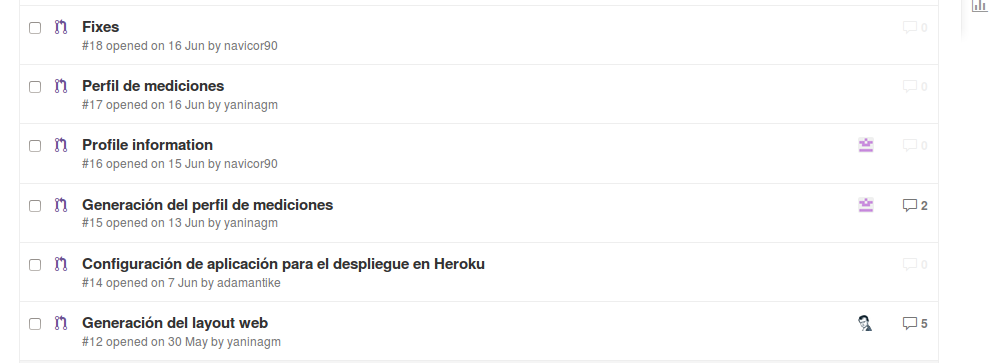
\includegraphics[width=.8\textwidth]{img/2-PR}
  \caption{Pull request realizados por el front end}
  \label{2-PR}
\end{figure}
\begin{figure}[h]
  \centering
  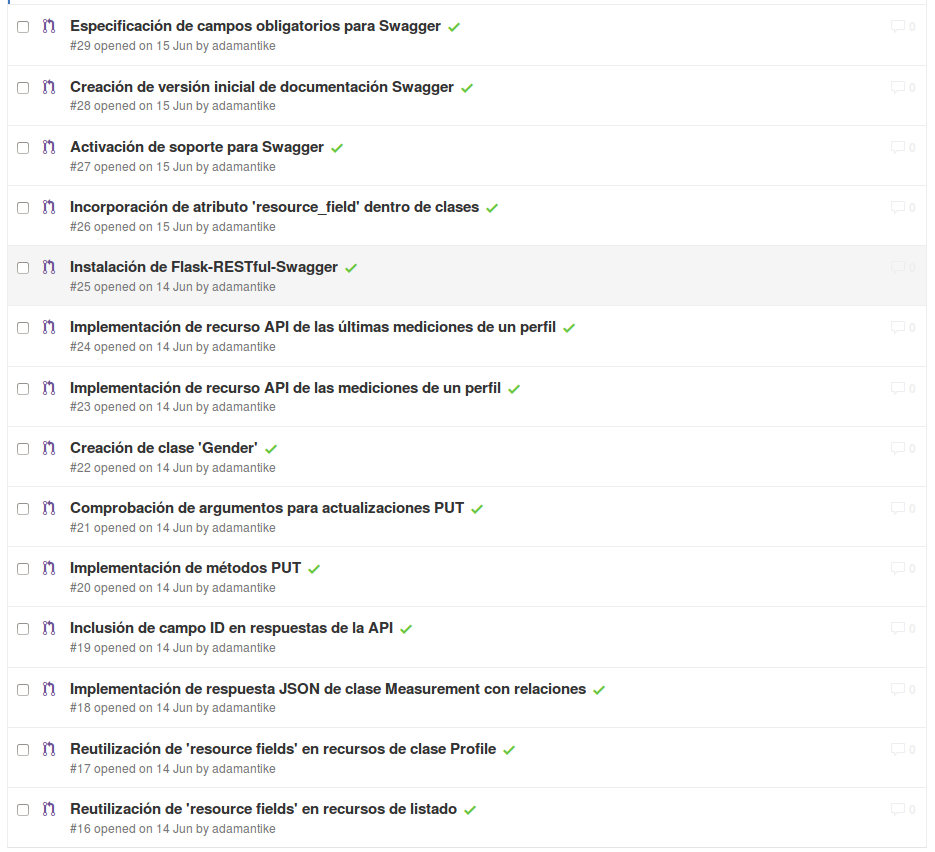
\includegraphics[width=.8\textwidth]{img/2-PR_back2}
  \caption{Pull request realizados por el back end -hoja1}
  \label{2-PR_back2}
\end{figure}
\begin{figure}[h]
  \centering
  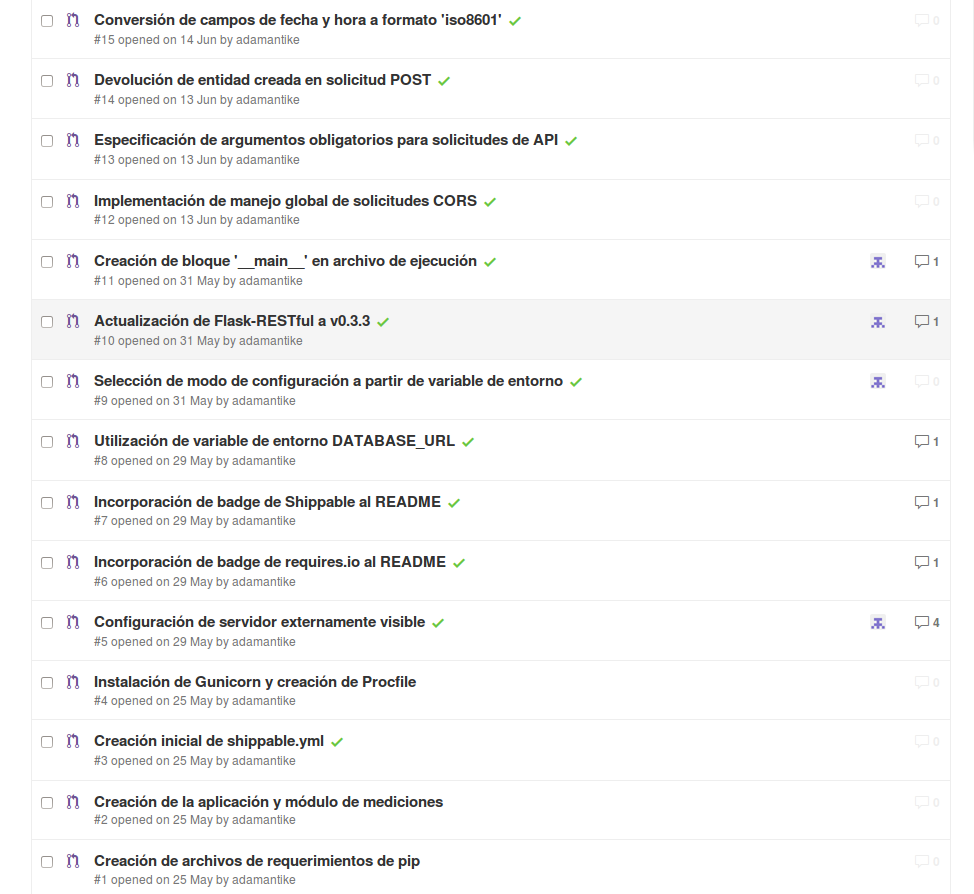
\includegraphics[width=.8\textwidth]{img/2-PR_Back}
  \caption{Pull request realizados por el back end -hoja2}
  \label{2-PR_Back}
\end{figure}

\clearpage
    
	{\scriptsize
	\begin{center} %sidewaystable
	\centering
	%\begin{adjustbox}{max width=\textheight}
    \resizebox{\textwidth}{!}{
	\begin{tabular}{|l|l|l|l|l|}
	    \hline
	        \textbf{Area a cargo} &
	        \textbf{Responsable} &        
	        \textbf{Tarea} &
	        \textbf{US} &
            \textbf{Tiempo dedicado} \\
	    \hline
	    Documentación& Yanina Morales &Trabajo práctico nº2 y avance de etapa de diseño &  & 20hs\\ \hline        
        Documentación& Ivan Terreno & Trabajo práctico nº2 y avance de etapa de diseño  &  & 20hs\\ \hline        
        Documentación& Michael Manganiello & Trabajo práctico nº2 y avance de etapa de diseño  &  & 20hs\\ \hline        
        Documentación& Franco Canizo & Trabajo práctico nº2 y avance de etapa de diseño  &  & 20hs\\ \hline         
	    Front-end& Michael Manganiello & Despliegue de la aplicación en heroku  & US-\ref{resumenInfo} \& US-\ref{infoSalud}& 4 hs  \\ \hline     
        Capacitación &Yanina Morales& Capacitación en utilización de angular de manera desacoplada& US-\ref{infoSalud}&12 hs\\ \hline        
        Capacitación &Ivan Terreno& Capacitación en utilización de angular de manera desacoplada& US-\ref{infoSalud}&12 hs\\ \hline                
	    Front-end& Ivan Terreno & Generación de controladores para consumir Json de la Api relacionados a la API & 8hs & US-\ref{resumenInfo} \& US-\ref{infoSalud} \\ \hline
        Front-end &Yanina Morales& Creación de página de formulario de carga de mediciones& US-\ref{infoSalud}&4hs\\ \hline
        Front-end&Ivan Terreno   & Creación de página de formulario de carga de perfil& US-\ref{infoSalud}&4hs\\ \hline
        Front-end&Ivan Terreno   & realización de pruebas& &8hs \\ \hline        
        Front-end&Yanina Morales   & realización de pruebas & & 12hs\\ \hline         
	
	    Back-end&Michael Manganiello  & Creación de modulo de mediciones&US-\ref{resumenInfo} \& US-\ref{infoSalud} &8hs\\ \hline
    	Back-end&Michael Manganiello  & Exposición de métodos como servicios de API 	& US-\ref{resumenInfo} \& US-\ref{infoSalud}&8hs\\ \hline
    	Back-end&Franco Canizo   & Adaptación de salida de métodos a formato Json&US-\ref{resumenInfo} \& US-\ref{infoSalud} &8hs\\ \hline
    	Back-end&Franco Canizo  & Carga de valores a la base de datos, relacionados a la API&US-\ref{resumenInfo} \& US-\ref{infoSalud} &8hs \\ \hline
    	Docuemntación&Franco Canizo  & Docuemntar las actividades realizadas& &16hs\\ \hline        
    	Docuemntación&Michael Manganiello  & Docuemntar las actividades realizadas& &16hs\\ \hline        
    	Docuemntación&Yanina Morales  & Docuemntar las actividades realizadas& &16hs\\ \hline        
    	Docuemntación&Ivan Terreno  & Docuemntar las actividades realizadas& &16hs\\ \hline                
	    \end{tabular}
        }
	    %\end{adjustbox}
    	\end{center}
	}
    
    
\subsection{Descripción}
En este sprint se llevaran a cabo las interfaces necesarias para que el usuario pueda cargar nuevas mediciones y ver todas sus últimas mediciones ,así teniendo un seguimiento de las mismas con posibilidad de que posteriormente pueda ver su evolución a través de gráficas y tablas.
Para la comunicación de estas interfaces con la API,se desarrollaran los correspondientes adaptadores para los recursos.

Para esto en el backend se deben preparar las clases Measurement, MeasurementType,MeasurementSource,MeasurementUnit con las debidas relaciones con las clase Profile desarrollada en el sprint anterior.
Para cada una de esas clases, se deben preparar interfaces de acceso a los recursos provistos por la API. Y su correspondiente documentación.


\subsection{User Stories relacionados}
La \textbf{Tabla \ref{US-Sprint1}} indicará las características de cada user story para guiarnos en el desarrollo del sprint.

\begin{table}[h]
	%\resizebox{\textwidth}{!}{
    \centering
	\begin{tabular}{|l|p{9cm}|c|}
	\hline
        \multicolumn{1}{|c|}{\textbf{ID}} &
        \multicolumn{1}{|c|}{\textbf{Enunciado de la historia}} &
        \textbf{Prioridad} \\          
    \hline
        US-\ref{resumenInfo} &
        Como paciente quiero obtener un resumen de mi información de salud básica para hacer uso de la misma en caso de una emergencia &Alta
        \\
    \hline 
	    US-\ref{infoSalud} &
        Como paciente quiero cargar mi información personal de salud referido a mediciones (altura, grasa corporal, peso, presión arterial), para que el médico cuente con más y mejor información al momento de realizar el diagnóstico. & Alta
        \\
    \hline
    \end{tabular}
%     }
    \label{US-Sprint1}
\end{table}


\begin{comment}
\subsection{Fase de Análisis}

En esta fase comenzaremos definiendo el Sprint backlog y describiendo en detalle cada una de las tareas que la componen, además se realizará un diagrama de clases iniciales (\textbf{Figura\ref{modelo_datos}}) que nos permitirá guiarnos durante el avance del sprint de ese modo obtener un sistema consistente. 
\end{comment}


\subsection{ Modelo de datos.}
El Diagrama propio de este sprint se puede ver en la \textbf{Figura\ref{2-modelo_datos_general}}, allí se indican exactamente las clases que se usarán en este sprint y que serán detalladas con detenimiento en el presente documento. Se recuerda que se ha realizado un Diagrama de clases tentativo que se puede ver en la \textbf{Figura \ref{2-modelo_datos_general}}, dicho diagrama  será utilizado como base para este sprint y posee un alcance limitado el cual se irá modificando a medida que se profundice en los temas.



\begin{figure}[h]
  \centering
  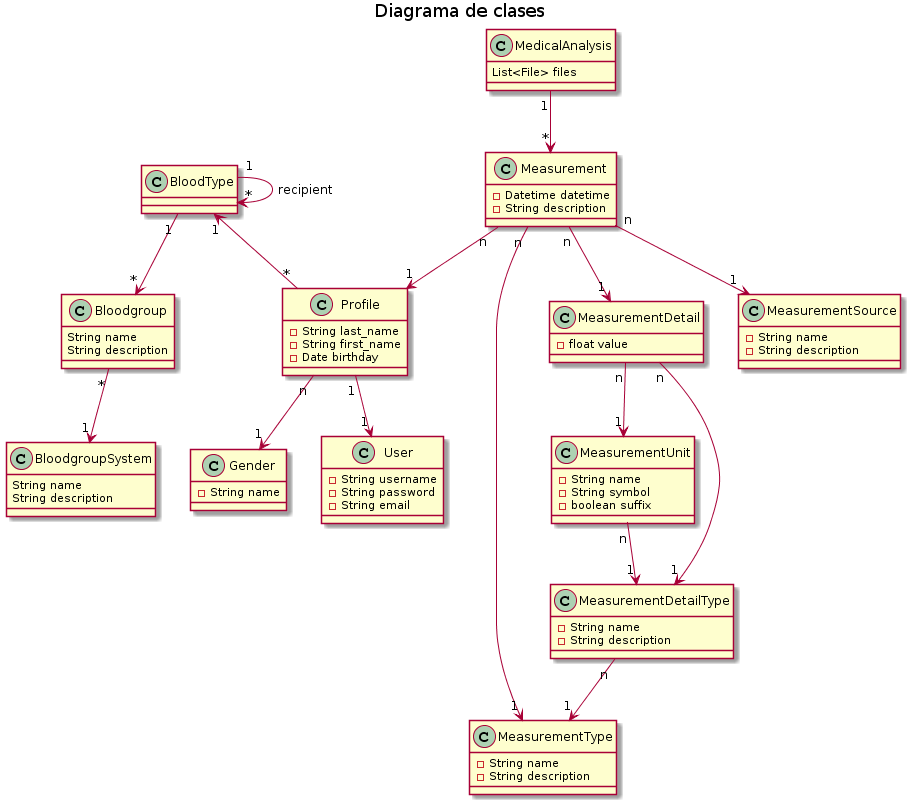
\includegraphics[width=.8\textwidth]{img/2-DC_especifico}
  \caption{Modelo de datos}
  \label{2-modelo_datos_general}
\end{figure}
\clearpage

\subsection{Descripción de las Clases}

\subsubsection{Clase Measurement} 
Dicha clase se refiere a las medición realizada por el usuario en un momento específico. 

\textbf{Descripción de los atributos}
	\begin{itemize}
		\item \textbf{id:} Identificador único de la medición (tipo int).
        \item \textbf{datetime:} Fecha y hora de la medición (tipo datetime).
        \item \textbf{value:} Valor de la medición (tipo float).
        \item \textbf{profile\_id:} Identificador único del perfil asociado (tipo int).
        \item \textbf{measurement\_source\_id:}Identificador único de la fuente de medición asociada (tipo int).
        \item \textbf{measurement\_type\_id:}Identificador único del tipo de medición asociado (tipo int).
        \item \textbf{measurement\_unit\_id:}Identificador único de la unidad de medición asociada (tipo int).
	\end{itemize}
    
\textbf{Dirección del recurso:}
\begin{lstlisting}[language=json,firstnumber=1]
<BASE URL>/measurements/{:id}
\end{lstlisting}

\textbf{Json generado por la API}    
\begin{lstlisting}[language=json,firstnumber=1]
{
    "resource": 
{
    "measurement_unit": 
{
    "symbol": "Kg",
    "suffix": true,
    "name": "Kilogramo",
    "id": 1
},
"measurement_source": 
{
    "name": "Manual",
    "description": null,
    "id": 1
},
"value": 50,
"measurement_type": 
{
    "name": "Peso",
    "description": "Peso corporal de la persona.",
    "id": 1
},
"id": 1,
"profile": 
{
    "birthday": "1990-10-26",
    "last_name": "Terreno",
    "first_name": "Milton",
    "gender": 
            {
                "name": "Masculino",
                "description": null,
                "id": 1
            },
            "id": 1
        },
        "datetime": "2015-06-15T02:29:54"
    }
}
\end{lstlisting}
\subsubsection{ Clase MeasurementType }
Esta clase nos permitirá  nomenclar  los tipos de medidas, hasta el momento hemos contemplado: peso, dimensión corporal (Ej:altura) y glucosa. Existen ciertas medidas que contemplan dos valores, estas serán agregadas en un sprint futuro.

\textbf{Descripción de los atributos}
    \begin{itemize}
			\item \textbf{name: }	Nombre del tipo de medición(tipo string).
            \item \textbf{description:} Descripción del tipo de medición (tipo string).
    \end{itemize}

\textbf{Dirección del recurso:}
\begin{lstlisting}[language=json,firstnumber=1]
<BASE URL>/measurement_types/{id}
\end{lstlisting}

\textbf{Json generado por la API} 
\begin{lstlisting}[language=json,firstnumber=1]
{
    "resource": 
    {
        "name": "Peso",
        "description": "Peso corporal de la persona.",
        "id": 1
    }
}
\end{lstlisting}

\subsubsection{ Clase MeasurementUnit }
Esta clase nos permitirá  nomenclar  las unidades de medicion disponible para que el usuario pueda seleccionarlas cdo realice la medición, hasta el momento hemos contemplado: Kilogramo, gramo, miligramos, metro, centimetro y milímetro.

    \textbf{Descripción de los atributos}
        \begin{itemize}
            \item \textbf{id:	}	Identificador único de la unidad de medición(tipo int).
            \item \textbf{name :	}	Nombre de la unidad de medición ( tipo string).
            \item \textbf{symbol :}		Símbolo de la unidad de medición (tipo string).
            \item \textbf{suffix :}	Variable booleana que indica si el símbolo de la unidad de medición es un sufijo (verdadero) o un prefijo (falso) del valor de la medición (tipo boolean).
        \end{itemize}

    \textbf{Dirección del recurso}
        \begin{lstlisting}[language=json,firstnumber=1]
        <BASE URL>/measurement_units/{id}
        \end{lstlisting}

    \textbf{Json generado por la API} 
        \begin{lstlisting}[language=json,firstnumber=1]
        {
            "resource": 
            {
                "symbol": "Kg",
                "suffix": true,
                "name": "Kilogramo",
                "id": 1
            }
        }
        \end{lstlisting}

\subsubsection{ Clase MeasurementSource}
Esta clase nos permitirá nomenclar los tipos de fuentes posibles como pueden ser manual, dispositivo móvil, sistema de salud y dispositivo de salud.
    
	\textbf{Descripción de los atributos}
        \begin{itemize}
            \item \textbf{name 	:}	Nombre de la fuente de medición (tipo string).
            \item \textbf{description 	:}	Descripción de la fuente de medición (tipo String).
        \end{itemize}
    \textbf{Dirección del recurso}
    \begin{lstlisting}[language=json,firstnumber=1]
    <BASE URL>/measurement_sources/{:id}
    \end{lstlisting}

    \textbf{Json generado por la API} 
    \begin{lstlisting}[language=json,firstnumber=1]
{
    "resource": 
    {
        "name": "Manual",
        "description": null,
        "id": 1
    }
}
    \end{lstlisting}
    
\subsection{ Modelo funcional.} %Diagrama de clases
Se describirán las funciones usando como marco de apoyo el sprint Backlog, además se armará el diagrama de casos de uso del presente Sprint \textbf{[Figura \ref{2-caso_de_uso}]} que irá creciendo  medida se vaya avanzando en el proyecto.
    \begin{figure}[h]
        \centering
        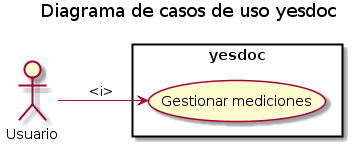
\includegraphics[width=0.5\textwidth]{img/2-caso_de_uso}
        \caption{formulario de edición de perfil}
		\label{2-caso_de_uso}
    \end{figure}

    
\subsubsection{Creación de página de mediciones}
En esta tarea  se generará la pantalla, \textbf{Figura \ref{perfil_medicion}} donde se muestran las mediciones del usuario, como lo son:
      \begin{itemize}
	      \item Altura
          \item Peso
          \item Grasa Corporal
          \item Presión Arterial
      \end{itemize}
      Al igual que en la creación del perfil se dará la posibilidad de acceder a la edición de su perfil desde esta misma página.
      
Para mostrarlas mediciones del usuario es necesario acceder al recurso \texttt{/profiles/\{profile\_id\}/measurements/latest} de la API a través de un método \textbf{GET}


      \textbf{Especificaciones del recursos \texttt{/measurements}}

    \begin{lstlisting}[language=json,firstnumber=1]
          MeasurementFields {
	measurement_source (MeasurementSourceFields, optional),
      profile (ProfileFields),
      datetime (date-time),
      value (number),
      measurement_unit (MeasurementUnitFields),
      id (integer),
      measurement_type (MeasurementTypeFields)
      }
      MeasurementSourceFields {
      description (string, optional),
      id (integer),
      name (string)
      }
      ProfileFields {
      first_name (string),
      last_name (string),
      id (integer),
      gender (GenderFields, optional),
      birthday (date-time, optional)
      }
      GenderFields {
      description (string, optional),
      id (integer),
      name (string)
      }
      MeasurementUnitFields {
      id (integer),
      symbol (string),
      suffix (boolean, optional),
      name (string)
      }
      MeasurementTypeFields {
      description (string, optional),
      id (integer),
      name (string)
      } 
    \end{lstlisting}

    En el perfil de usuario se mostrarán de cada tipo de medición que ha realizado el usuario la última de cada una, indicando el nombre, el valor, el simbolo, la fecha y hora y el método con el que ha sido realizada la medición. Además para cada una de las mediciones se mostrarán dos iconos que corresponden a la edición y a la compartición de las mediciones, este último será implementado en un sprint futuro.

    \begin{figure}[h]
        \centering
        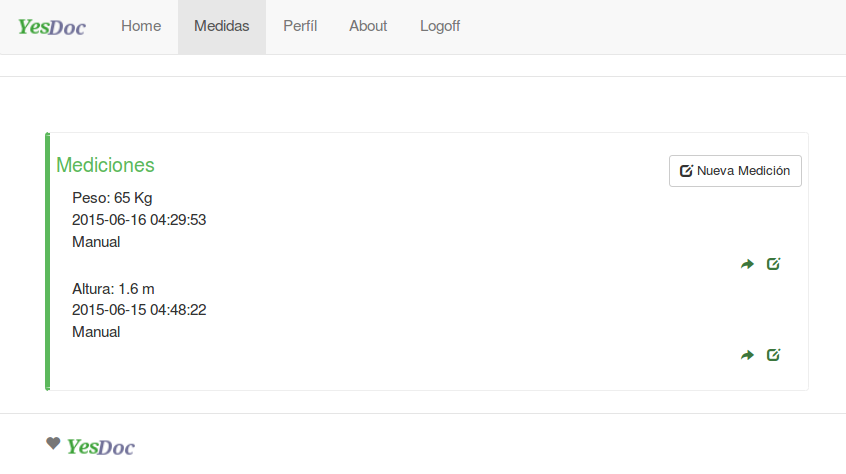
\includegraphics[width=1\textwidth]{img/2-perfil_medicion}
        \caption{Perfil de mediciones}
		\label{perfil_medicion}
    \end{figure}
    
\subsubsection{ Creación de página de formulario de carga de mediciones}
Se generará el formulario necesario, que se muestra en la \textbf{Figura \ref{nueva_medicion}} para que el usuario pueda cargar las mediciones antes nombrados, para ello es necesario acceder al recurso \texttt{/measurements} de la API a través de un método \textbf{POST}

      \begin{lstlisting}[language=json,firstnumber=1]
         MeasurementFields {
        measurement_source (MeasurementSourceFields, optional),
        profile (ProfileFields),
        datetime (date-time),
        value (number),
        measurement_unit (MeasurementUnitFields),
        id (integer),
        measurement_type (MeasurementTypeFields)
        }
        MeasurementSourceFields {
        description (string, optional),
        id (integer),
        name (string)
        }
        ProfileFields {
        first_name (string),
        last_name (string),
        id (integer),
        gender (GenderFields, optional),
        birthday (date-time, optional)
        }
        GenderFields {
        description (string, optional),
        id (integer),
        name (string)
        }
        MeasurementUnitFields {
        id (integer),
        symbol (string),
        suffix (boolean, optional),
        name (string)
        }
        MeasurementTypeFields {
        description (string, optional),
        id (integer),
        name (string)
        } 
    \end{lstlisting}
    
Desde el perfil de mediciones se presentará un icono que representa a la creación de un elemento para que el usuario pueda seleccionarlo. Esta acción llevara al usuario al formulario de creación de mediciones, donde los campos estarán vacios, para que el usuario los cargue con los valores correspondientes. Una vez terminada la carga, se mostrará un mensaje avisando al usuario que se ha realizado con éxito y luego lo redireccionará al perfil de mediciones.
    
    \begin{figure}[h]
        \centering
        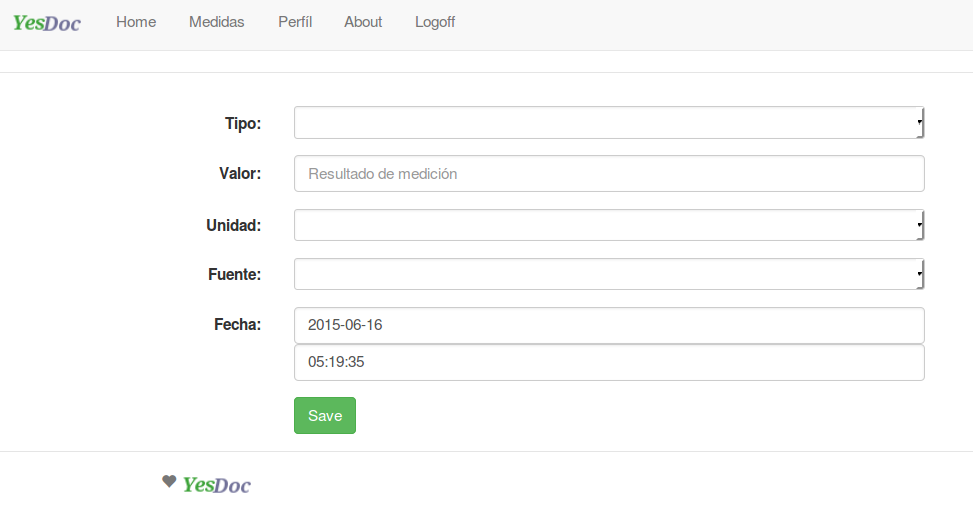
\includegraphics[width=1\textwidth]{img/2-nueva_medicion}
        \caption{Formulario de nueva medición}
		\label{nueva_medicion}
    \end{figure}
\subsubsection{ Creación de página de formulario de edición de mediciones}
Se generará el formulario necesario, que se muestra en la \textbf{Figura \ref{editar_medicion}} para que el usuario pueda editar una medición previamente seleccionada, para ello es necesario acceder al recurso \texttt{/measurements/\{:id\}} a través del método \textbf{PUT} enviando por URL el id correspondiente a dicha medición. 

Desde el perfil de mediciones se presentará un icono que representa a la edición de un elemento para que el usuario pueda seleccionarlo. Esta acción llevara al usuario al formulario de edición de mediciones, donde los campos estarán cargados con los valores antiguos, de este modo el usuario modifica lo que desea y no tiene que cargar todo nuevamente. Una vez terminada la edición se redireccionará al perfil de mediciones.

	\begin{figure}[h]
        \centering
        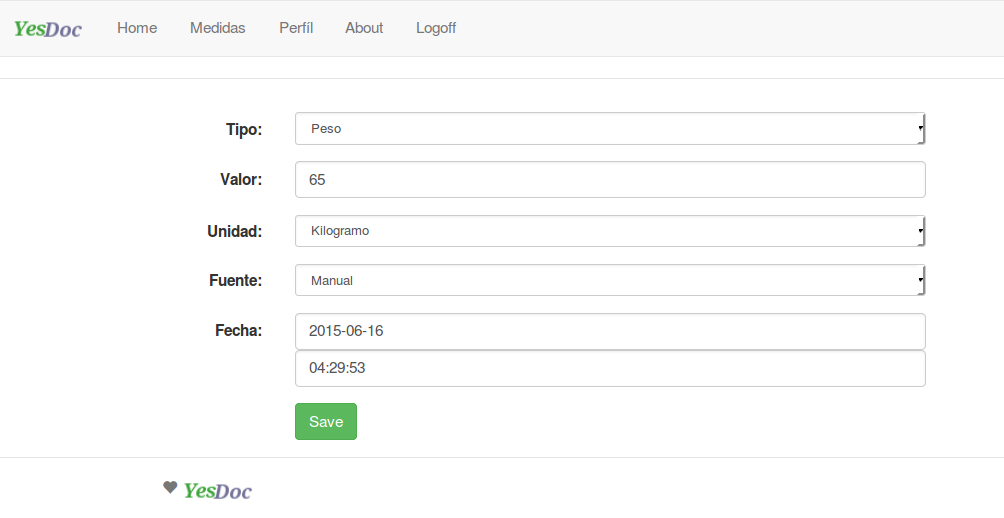
\includegraphics[width=1\textwidth]{img/2-editar_medicion}
        \caption{Formulario de edición de medición}
		\label{editar_medicion}
    \end{figure}
    
%%%%%%%%%%%%%%%%%%%%%% COMPLETAR!!! %%%%%%%%%%%%%%%%%%%%%%%%%%%%
\begin{comment}


\subsubsection{Creación de aplicación  }
\subsubsection{Creación de modulo de mediciones}
\subsubsection{Exposición de métodos como servicios de API}
\subsubsection{ Adaptación de salida de métodos a formato Json}
\subsubsection{Creación de base de datos inicial}
\end{comment}

\subsection {Salidas del Sistema - Incrementos}

Luego de finalizado este user story se obtendrán 4 pantallas que se detallarán a continuación:
\begin{enumerate}
    \item \textbf{Presentación de las últimas mediciones}  \textbf{[Figura  \ref{perfil_medicion}]} con posibilidad de edición de cada una de las mediciones. Los datos posible  a presentar son altura, peso, grasa corporal y glucosa. 
    
    La interfaz mostrará el valor de la medición, la fecha y hora en que fue realizada y la fuente que se utilizó para dicha medición.
	\item \textbf{Carga de mediciones}: \textbf{[Figura \ref{nueva_medicion}]} Se le permitirá cargar mediciones que realice en algún momento del día como son peso, altura, grasa corporal y glucosa. Deberá indicar la fuente, tipo, unidad y fecha de la medición
    \item \textbf{Edición de mediciones:}  \textbf{[Figura \ref{editar_medicion}]} Se le permitirá seleccionar una medición del perfil de mediciones para sel modificada.

\end{enumerate}

    




\subsection{Criterios de aceptación}

\begin{center}
\begin{longtable}{|p{0.5cm}|p{4cm}|p{4cm}|p{5cm}|}
\hline \hline \rowcolor[gray]{0.9}
	\multicolumn{4}{||c|}{\textbf{Criterio de aceptación}} \\
    \hline  \rowcolor[gray]{0.9}
        \textbf{Id} &
        \textbf{Contexto} &
        \textbf{Evento}&
        \textbf{Resultado} \\
    \hline
1&En caso de que exista una persona sin mediciones & cuando este desee observar sus mediciones  & El sistema no mostrará nada \\ \hline
 
2& Cuando el usuario registrado ingresa dos mediciones del mismo tipo  & y luego quiera consultarlas & El sistema solo le mostrará la ultima medición, del mismo tipo, realizada\\ \hline

3& Cuando el usuario seleccione una medición & y luego quiera editarla & El sistema le permitira la correspondiente edición\\ \hline

4& Si el usuario existe y no está logeado & y quiera ingresar a ver sus mediciones. & El sistema no le permitirá ingresar\\ \hline
  \end{longtable}
\end{center}


\subsection{Casos de Prueba}


	{\scriptsize
	\begin{table}[h]
	\centering
	\begin{tabular}{||l|p{10cm}||}
    	\rowcolor[gray]{0.9}
	    \hline 
        \hline 
	    \textbf{Caso de prueba} & \textbf{Consultar mediciones (sin medidas precargadas)}\\  \hline
	    \textbf{Descripción del escenario}& Nombre: Marita; Apellido Martinez; fecha de Nacimiento:20-08-1989; id:3  \\ \hline
	    \textbf{Criterio de aceptación}&  \textbf{En caso de que exista una persona sin mediciones cargadas, si el usuario desea verlas el sistema no debería mostrar ninguna medición } \\ \hline
        \textbf{Datos de entrada}&  consultar mediciones\\ \hline
        \textbf{Condiciones de  prueba}& Se necesita que esté previamente cargado el usuario "Marita Martinez" y no tenga datos más allá de su nombre y apellido en el perfil \\ \hline \hline
	    \end{tabular}
        \caption{Caso de prueba para criterio de aceptación 1}
    	\end{table}
	}
  
{\scriptsize
	\begin{table}[h]
    \centering
	\begin{longtable}{|p{5cm}|p{5cm}|p{5cm}|}
	    \hline \hline \rowcolor[gray]{0.9}
        \multicolumn{3}{||l|}{\textbf{Procedimiento de Prueba - ``Consultar mediciones''}} \\
        \hline \rowcolor[gray]{0.9}
		    \textbf{Actor} & 
	        \textbf{Sistema}& 
        	\textbf{Resultado Esperado} \\  
        \hline
	    El usuario ingresa al sistema con su id nº3	& &\\ \hline
        		& El sistema valida con los perfiles de la API si el Id:3 del usuario existe& Se presenta por pantalla el perfil del usuario con sus datos  \\ \hline        
	    El usuario selecciona la pestaña mediciones y realiza la consulta& &\\ \hline
      	&El sistema valida que las cookies estén activas&\\ \hline
   		&El sistema solicita a la API las mediciones del perfil con id:3&El sistema no muestra ninguna medida cargada \\ \hline 
	    \end{longtable}
		\caption{Procedimiento de prueba para criterio de aceptación 1}
    	\end{table}
	}
    
        {\scriptsize
	\begin{table}[h]
	\centering
	\begin{tabular}{|l|p{10cm}|}
	    \hline 
	    \textbf{Salida obtenida}& No se presentan datos de mediciones\\ \hline
	    \textbf{Resultado}& \textbf{Correcto}\\ \hline
        \textbf{¿Que fue mal?}& Nada\\ \hline      
        \textbf{Evidencia}& \\ \hline
        \textbf{Seguimiento}&No es necesario ya que el caso de prueba no causó
fallos \\ \hline
        \textbf{Estado}& \textbf{Terminado}\\ \hline        
         \textbf{¿Que se puede mejorar?}& En otra itreación se debería añadir carteteles de avisos, informando que faltan cargar datos \\ \hline              
	    \end{tabular}
        \caption{Resultado esperado para el criterio de aceptación 1}
    	\end{table}
	}
\clearpage 
%%%%%%%%%%%%%%%%%%%%%%%%%%%%%%%%%%%%%%%%%%%%%%%%%%

{\scriptsize
	\begin{table}[h]
	\centering
	\begin{tabular}{||l|p{9cm}||}
    	\rowcolor[gray]{0.9}
	    \hline 
        \hline 
	    \textbf{Caso de prueba}  &  \textbf{Consultar mediciones (medida precargada)}\\  \hline
	    \textbf{Descripción del escenario}& Nombre: Marita; Apellido Martinez; fecha de Nacimiento:20-08-1989; id:3; altura: 2m  \\ 			\hline
	    \textbf{Criterio de aceptación} &\textbf{ Cuando el usuario registrado ingresa dos mediciones del mismo tipo y luego quiera consultarlas. El sistema solo le mostrará la ultima medición, del mismo tipo, realizada} \\ \hline
        \textbf{Datos de entrada}& id:3; Peso 1: 67kg; peso 2: 55kg \\ \hline
        \textbf{Condiciones de  prueba}& el usuario Marita Martinez existe \\ \hline 			\hline
	    \end{tabular}
        \caption{Caso de prueba para criterio de aceptación 2}        
	    \end{table}
}
 
   %{\scriptsize
	\begin{longtable}{|p{5cm}|p{5cm}|p{4cm}|}
 
	    \hline \hline \rowcolor[gray]{0.9}
        \multicolumn{3}{||l|}{\textbf{Procedimiento de Prueba - Consultar mediciones}} \\ \hline
	    \hline 
        \rowcolor[gray]{0.9}
	    \textbf{Actor} & \textbf{Sistema}& \textbf{Resultado Esperado} \\  \hline
	    El usuario se logea en el sistema& & \\ \hline
        & El sistema consulta la API para corroborar que el perfil con id:3 existe &\\ \hline
        &  El sistema redirecciona al usuario a la vista de perfil de usuario&Se muestra el perfil de usuario con los datos respectivos\\ \hline
	    El usuario selecciona la pestaña de mediciones de la barra de navegación& &\\ \hline
        & El sistema verifica las cookies del usuario para determinar si ya se encuentra logeado &\\ \hline
        & El sistema redirecciona al usuario a la vista de mediciones&Se muestra la vista de mediciones con las últimas mediciones del usuario correspondientes\\ \hline  
        El usuario selecciona el botón de añadir ``nueva medicion''& &\\ \hline       
        & El sistema verifica que las cookies posean los datos del usuario&\\ \hline       
        & Se redirecciona a la vista de carga de mediciones&Se presenta el formulario de medición para la carga respectiva\\ \hline
        El usuario selecciona: Tipo de medicion: Peso; medida 55; unidad: Kg; Fuente: manual; fecha: deja la precargada y  luego de esto presiona el botón save& &\\ \hline       
        & El sistema valida que estén todos los datos cargado, excepto fuente el cual no es necesario, carga los nuevos datos en la API a través del método POST y redirecciona a la vista de mediciones&\\ \hline       
        &El sistema a través del método GET trae las últimas mediciones. &Se muestran las últimas mediciones en la vista de mediciones\\ \hline
        El usuario presiona el botón ´´cargar mediciones'' nuevamente& &\\ \hline  
        & El sistema verifica que las cookies posean los datos del usuario&\\ \hline       
        & Se redirecciona a la vista de carga de mediciones&Se presenta el formulario de mediciones para la carga respectiva\\ \hline
        El usuario selecciona: Tipo de medicion: Peso; medida 67; unidad: Kg; Fuente: manual; fecha: deja la precargada y  luego de esto presiona el botón save& &\\ \hline       
        & El sistema valida que estén todos los datos cargado, excepto fuente el cual no es necesario, carga los nuevos datos en la API a través del método POST y redirecciona a la vista de mediciones&\\ \hline       
        &El sistema a través del método GET trae las últimas mediciones. &El sistema muestra la última medición cargada ``Peso 55 Kg, fecha de carga y método: manual\\ \hline
        \caption{Procedimiento de prueba para criterio de aceptación 2}
        
	    \end{longtable}
        
	%}
\clearpage

{\scriptsize
	\begin{table}[h]
	\centering
	\begin{tabular}{|l|p{10cm}|}
	    \hline 
	    \textbf{Salida obtenida}& Se mostraron correctamente la ultima medición del mismo tipo\\ \hline
	    \textbf{Resultado}& \textbf{Correcto}\\ \hline
        \textbf{¿Que fue mal?}& Nada\\ \hline      
        \textbf{Evidencia}& En Listing \ref{JsonMediciones} se puede observar que el usuario posee 3 mediciones, dos de las cuales son del mismo tipo (tipo Peso) y en la Figura \ref{perfil_id_3} se puede ver que solo se muestra la última medición del Peso.  \\ \hline
        \textbf{Seguimiento}& no es necesario\\ \hline
        \textbf{Estado}& \textbf{Terminado}\\ \hline        
        \textbf{¿Que se puede mejorar?}& \\ \hline              
	    \end{tabular}
        \caption{Resultado esperado para el criterio de aceptación 2}
    	\end{table}
	}


{\scriptsize
%\begin{minipage}{1 \textwidth}
    \begin{lstlisting}[language=json,firstnumber=1,  breaklines=true, caption= Json de las mediciones del perfil id:3, label=JsonMediciones]

        {"resource": 
	        [{
	    	    "measurement_source": 
        		{
		            "id": 1,
        		    "description": null,
		            "name": "Manual"
        		},
		        "measurement_type": 
        		{
		            "id": 1,
		            "description": "Peso corporal de la persona.",
		            "name": "Peso"
		        },
        		"datetime": "2015-07-03T11:51:39.436000",
		        "value": 55,
		        "id": 16,
    	    	"measurement_unit": 
                {
             	   "id": 1,
	               "suffix": true,
	               "name": "Kilogramo",
	               "symbol": "Kg"
	             }
    	    },
        	{
            	"measurement_source": 
		        {
        		    "id": 1,
		            "description": null,
		            "name": "Manual"
		        },
	        	"measurement_type": 
    		    {
	        	    "id": 1,
		            "description": "Peso corporal de la persona.",
		            "name": "Peso"
		        },
        		"datetime": "2015-07-03T11:54:22.806000",
		        "value": 67,
		        "id": 17,
        	"measurement_unit": 
	            {
    	            "id": 1,
        	        "suffix": true,
            	    "name": "Kilogramo",
                	"symbol": "Kg"
                }
              },
              {"measurement_source": 
                {
                    "id": 0,
                    "description": null,
                    "name": null
                },
               "measurement_type": 
                {
                    "id": 2,
                    "description": "Longitud de la persona",
                    "name": "Altura"
                },
	                "datetime": "2015-07-03T13:05:57.375000",
    	            "value": 2,
        	        "id": 18,
                "measurement_unit": 
                    {
                        "id": 2,
                        "suffix": true,
                        "name": "Metros",
                        "symbol": "m"
                    }
    	    }]
        }   
    \end{lstlisting}   


\begin{figure}[h]
        \centering
        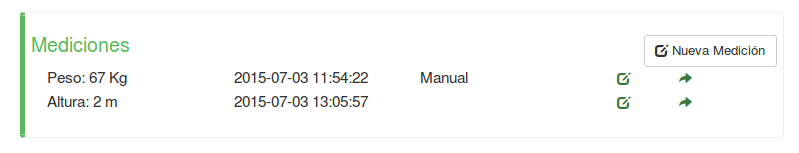
\includegraphics[width=1\textwidth]{img/2-prueba_2}
        \caption{perfil de medicion de usuario con id:3}
		\label{perfil_id_3}
\end{figure}


%\end{minipage}
    }
\clearpage

%%%%%%%%%%%%%%%%%%%%%%%%%%%%%%%%%%%%%%%%%%%%%%%%%%%%%%%%%

{\scriptsize
	\begin{table}[h]
	\centering
	\begin{tabular}{||l|p{10cm}||}
    	\rowcolor[gray]{0.9}
	    \hline 
        \hline 
	    \textbf{Caso de prueba} & \textbf{Editar Medición}\\  \hline
	    \textbf{Descripción del escenario}&  Nombre: Marita; Apellido Martinez; fecha de Nacimiento:20-08-1989; id:3; id:3; Peso 1: 67kg, id:17; peso 2: 55kg, id:16\\ \hline
	    \textbf{Criterio de aceptación}& \textbf{Cuando el usuario seleccione una medición  y luego quiera editarla. El sistema le permitira la correspondiente edición}\\ \hline
        \textbf{Datos de entrada}& peso:65Kg \\ \hline
        \textbf{Condiciones de  prueba}& Usuario logeado con al menos una medida cargada \\ \hline \hline
	    \end{tabular}
	    \end{table}
	}
    

	\begin{longtable}{|p{5cm}|p{5cm}|p{4cm}|}
	    \hline \hline \rowcolor[gray]{0.9}
        \multicolumn{3}{||l|}{\textbf{Procedimiento de Prueba - Editar mediciones}} \\ \hline
	    \hline 
        \rowcolor[gray]{0.9}
	    \textbf{Actor} & \textbf{Sistema}& \textbf{Resultado Esperado} \\  \hline
	    El usuario, ya logeado selecciona el botón de editar de una de las mediciones (medición peso 67Kg) que se muestra en su perfil de mediciones& & \\ \hline
        & El sistema valida las que las cookies estén activas & \\ \hline
        & El sistema consulta a la API la medición 17 correspondiente al perfil con id:3 & Se muestra el perfil del formulario de carga de mediciones. con los datos precargados de la medición seleccionada\\ \hline        
	    El usuario modifica los datos de la medición seleccionada cambiando 67 por 65&  &\\ \hline
        & el sistema confirma la carga guardando los datos en la API a través del método PUT&\\ \hline
        &El sistema redirecciona al usuario a la vista de perfil de mediciones&  Se le presenta al usuario la vista de las ultimas mediciones realizadas. Mostrando 65Kg \\ \hline
        		\caption{Procedimiento de prueba para criterio de aceptación 3}
	    \end{longtable}
	
            {\scriptsize
	\begin{table}[h]
	\centering
	\begin{tabular}{|l|p{10cm}|}
	    \hline 
	    \textbf{Salida obtenida}& La vista presento la medición modificada de forma correcta\\ \hline
	    \textbf{Resultado}& \textbf{Correcto}\\ \hline
        \textbf{¿Que fue mal?}& Nada\\ \hline      
        \textbf{Evidencia}&  En la figura \ref{edicion_medicion} se puede ver como el formulario se encuentra precargado con los valores de la medición que se desea editar, en el Json \ref{JsonMedicionModificada} se puede observar que se modifico el valor del peso y que ha cambiado la fecha de carga \\ \hline
        \textbf{Seguimiento}& No es necesario ya que el caso de prueba no causó
fallos\\ \hline
        \textbf{Estado}& \textbf{Terminado}\\ \hline        
        \textbf{¿Que se puede mejorar?}& En otro sprint se debería añadir carteles de avisos, informando que la edición fue realizada con éxito \\ \hline              
	    \end{tabular}
        \caption{Resultado esperado para el criterio de aceptación 3}
    	\end{table}
	}
\begin{figure}[h]
        \centering
        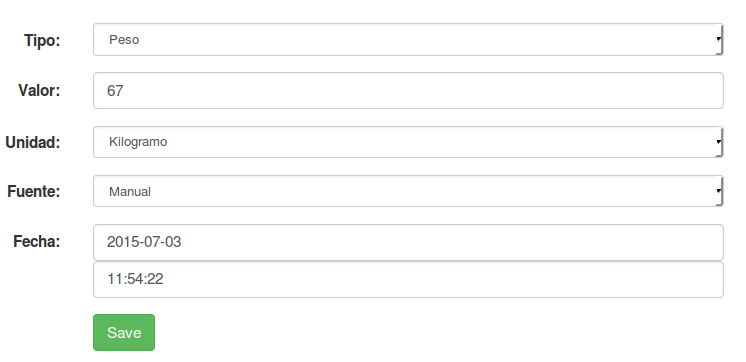
\includegraphics[width=1\textwidth]{img/2-prueba_3}
        \caption{Formulario de edición de medición}
		\label{edicion_medicion}
\end{figure}

\begin{lstlisting}[language=json,firstnumber=1,  breaklines=true, caption= Json de las medicion modificada del perfil id:3, label=JsonMedicionModificada]
{
	"id": 17,
    "measurement_source": 
	{
    	"id": 1,
	    "description": null,
	    "name": "Manual"
	},
	"measurement_unit": 
	{
    "id": 1,
    "suffix": true,
    "symbol": "Kg",
    "name": "Kilogramo"
	},
	"measurement_type": 
    {
        "id": 1,
        "description": "Peso corporal de la persona.",
        "name": "Peso"
    },
    "value": 65,
    "datetime": "2015-07-03T11:54:22.806000"
}
\end{lstlisting}
\clearpage  

%%%%%%%%%%%%%%%%%%%%%%%%%%%%%%%%%%%%%%%%%%%%%%%%%%%%%%%%%
		{\scriptsize
    \begin{table} [h]
    \centering
	\begin{tabular}{||l|p{10cm}||}
    	\rowcolor[gray]{0.9}
	    \hline 
        \hline 
		\textbf{Caso de prueba} & \textbf{Ingresar a mediciones} \\  \hline
	    \textbf{Descripción del escenario}& Nombre: Marita; Apellido Martinez; fecha de Nacimiento:2015-06-01; género: femenino; id:3; Peso 1: 54kg; peso 2: 55kg\\ \hline
	    \textbf{Criterio de aceptación}&\textbf{Si el usuario existe y no está logeado y quiere ingresar a ver sus mediciones. El sistema no le permitirá ingresar}\\ \hline
        \textbf{Datos de entrada}&  \\ \hline
        \textbf{Condiciones de  prueba}& El usuario no debe encontrase logeado.\\ \hline \hline
	    \end{tabular}
        \caption{Caso de prueba para criterio de aceptación 4}
    	\end{table}
		}
	

	\begin{longtable}{|p{5cm}|p{5cm}|p{5cm}|}
	    \hline \rowcolor[gray]{0.9}
        \multicolumn{3}{|l|}{\textbf{Procedimiento de Prueba -Ingresar mediciones}} \\ \hline
	    \textbf{Actor} & \textbf{Sistema}&\textbf{Resultado Esperado} \\  \hline
	   El usuario selecciona la pestaña de mediciones, para ver sus mediciones & & \\ \hline
        & El sistema  verifica que exita una cookie activa como na existe no lo redirección a ninguna parte &  Se muestra la ventana de logeo \\ \hline
   \caption{Procedimiento de prueba para criterio de aceptación 4}        
    \end{longtable}
 


{\scriptsize
	\begin{table}[h]

	\centering
	\begin{tabular}{|l|p{10cm}|}
	    \hline 
	    \textbf{Salida obtenida}&Se obtuvo lo q se esperaba, ya que no fue enviado a la interface de mediciones.\\ \hline
	    \textbf{Resultado}& \textbf{Correcto}\\ \hline
        \textbf{¿Que fue mal?}& Nada\\ \hline        
        \textbf{Evidencia}&No es necesaria  \\ \hline
        \textbf{¿Que fue mal?}& Nada\\ \hline      
        \textbf{Seguimiento}& No es necesario ya que el caso de prueba no causó fallos \\ \hline
        \textbf{Estado}& \textbf{Terminado}\\ \hline        
        \textbf{¿Que se puede mejorar?}& En una futura iteración se podría añadir carteles de avisos informando de la situación\\ \hline              
	    \end{tabular}
        \caption{Resultado esperado para el criterio de aceptación 4}
   	\end{table}
	}

%%%%%%%%%%%%%%%%%%%%%%%%%%%%%%%%%%%%%%%%%%%%%%%%%%%%%%%%%%%%%%%%%%

\clearpage
\subsubsection{Pruebas  de  integración  entre módulos del Sistema}
Estas pruebas se realizarán mas adelantes
\subsubsection{ Pruebas de carga}
En este sprint no se realizarán este tipo de pruebas.
\subsubsection{ Pruebas de seguridad por niveles de usuarios}
En este sprint no se realizarán este tipo de pruebas, ya que la seguridad será un tema a tratar más adelante.

\subsection{Pruebas ejecutadas}
Aqui se realizará una conclusión general de lo que se descubrió en las pruebas.
        %
	\begin{itemize}
		\item \textbf{¿Que fue bien?}
        	\begin{itemize}
				\item        Las cargas y ediciones se llevan a cabo correctamente.
			\end{itemize}

   		\item \textbf{¿Que se mejoró?}
        	\begin{itemize}
				\item \textbf{Cerrado} Al crear una nueva medición, se mostraba un cartel (alert de javascript) con una fecha, dicho alert fue eliminado.
                \item \textbf{Cerrado} Se encontró un problema con la zona horaria que usa el servidor y la zona horaria del usuario, para solucionarlo hubo q hacer un casteo previo cuando se solicitaba la fecha y hora del usuario para mostrar.
			\end{itemize}

   		\item \textbf{¿Que se puede mejorar?}
        	\begin{itemize}
		        \item \textbf{Abierto} En el futuro se deberá mejorar las validaciones de los datos a la hora de cargar información en los formularios.
        		\item \textbf{Abierto} Se deberá mejorar la manera de seleccionar la fecha y la hora.
		        \item \textbf{Abierto} Solo debería mostrarse las unidades relacionadas al tipo de medición que se ha seleccionado  
                \item \textbf{Abierto} Deberá realizarse los carteles de advertencia necesarios.
            \end{itemize}
        

	\end{itemize}


%%%%%%%%%%%%%%%%%%%%%%%%%%      FIN SPRINT 2  %%%%%%%%%%%%%%%%%%%%%%%%%

\section{Sprint 3: }%Corrección de issues 
\subsection{Planificación}

\textbf{Inicio: }Martes 7 de julio del 2015 

\textbf{Fin:} Martes 16 de Agosto del 2015

\begin{figure}[h!]
  \centering
  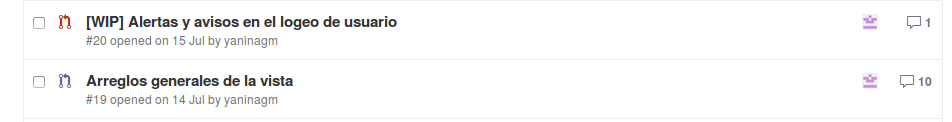
\includegraphics[width=.8\textwidth]{img/3-PR_1_front}
  \caption{Pull request realizados en el sprint  3}
  \label{pull_request_sprint_3}
\end{figure}
\begin{figure}[h!]
  \centering
  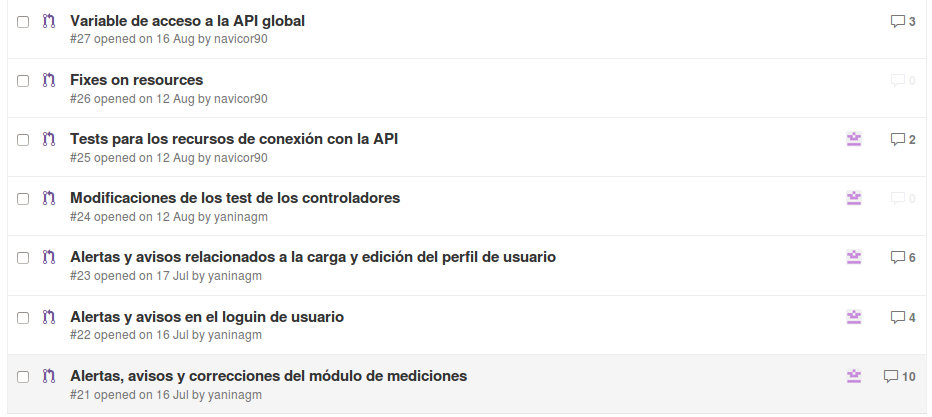
\includegraphics[width=.8\textwidth]{img/3-PR_2_front}
  \caption{Pull request realizados en el sprint  3}
  \label{3-PR_back}
\end{figure}

	{\scriptsize
	\begin{center} %sidewaystable
	\centering
	%\begin{adjustbox}{max width=\textheight}
    \resizebox{\textwidth}{!}
    {
	\begin{tabular}{|l|l|p{5cm}|l|l|}
	    \hline
	        \textbf{Area a cargo} &
	        \textbf{Responsable} &        
	        \textbf{Tarea} &
	        \textbf{US} &
            \textbf{Tiempo}\\
   		\hline
       
	    Documentación& Michael Manganiello & trabajo práctico integrador nº2 ``Planificación de proyectos informáticos''. & & 17hs \\ \hline
        Documentación& Ivan Terreno & trabajo práctico integrador nº2 ``Planificación de proyectos informáticos''. & & 17hs \\ \hline
        Documentación& Morales Yanina & trabajo práctico integrador nº2 ``Planificación de proyectos informáticos''. & & 17hs \\ \hline
        Documentación& Franco Canizo & trabajo práctico integrador nº2 ``Planificación de proyectos informáticos''. & & 17hs \\ \hline
        Presentaciones& Todos & Postulación del proyecto la BAIT 2015. & & 4hs \\ \hline
        Presentaciones& Todos & Preparación de la presentación en BAIT 2015. & & 15hs \\ \hline        
	    Front-end& Yanina Morales & Creación de validadores y mensajes de alerta & & 10hs\\ \hline             
	    \end{tabular}
        }
	    %\end{adjustbox}
    	\end{center}
	}


\subsection{Descripción}
%navbar responsive
En este sprint se corregirán los errores detectados en las pruebas realizadas con anterioridad en los sprint referidos a:
    \begin{itemize}
    \item Generar perfil de datos personales.
    \item Generar  perfil de mediciones.
    \end{itemize}
Cabe destacar que sólo se documentarán aquellas correcciones que se refieran a las funcionalidades a documentar ``Carga y muestra de mediciones''

Se desarrollarán las interfaces que permiten mostrar las gráficas de ñas mediciones de un usuario.

Y se realizarán las validaciones necesarias para que el sistema funcione correctamente.


Además en este Sprint el equipo se presentó y quedó como finalista en el  concurso ``Premio a la Innovación Tecnológica'', organizado por el Polo IT de Buenos Aires, teniendo que organizar la presentación a mostrar. Para ellos se realizó un video de presentación, una página web, tarjetas de contacto y se preparo un speech elevator para conquistar al público


\subsection{User Stories relacionados}
La \textbf{Tabla \ref{US-Sprint3} } indicará las características de cada user story para guiarnos en el desarrollo del sprint.

\begin{table}[h]
    \label{US-Sprint3}
	%\resizebox{\textwidth}{!}{
    \centering
	\begin{tabular}{|l|p{9cm}|}
	\hline
        \multicolumn{1}{|c|}{\textbf{ID}} &
        \multicolumn{1}{|c|}{\textbf{Enunciado de la historia}} \\          
    \hline
        \textbf{US-2 } & Como paciente, quiero añadir al sistema los estudios realizados para evitar posibles perdidas.\\
     \hline 
        \textbf{US-5 } & Como paciente quiero que los sistemas de salud existentes puedan cargar sus resultados directamente en mi carpeta de salud para centralizar mi información. \\
      \hline 
        \textbf{US-7} & Como paciente quiero categorizar mis estudios por rama de medicina, para lograr una mejor organización y navegabilidad en el sistema. \\
       \hline 
        \textbf{US-8} & Como laboratorio, quiero cargar información de un paciente en su cuenta para ahorrarle las molestias de volver. \\
        \\
    \hline 
	    \textbf{US-17} &   Como paciente quiero ver gráficas que resuman mi información en particular para poder ver mis cambios a lo largo de la historia.\\
    \hline        
        \textbf{US-15} & Como médico quiero ver gráficas que resuman la información de un paciente para poder ver sus cambios a lo largo de la historia y así apoyar la toma de decisiones y el diagnóstico.\\
    \hline
    \end{tabular}
%     }

\end{table}

\subsection{Clases involucradas}
\label{3-clases_involucradas}
\begin{figure}[h!]
	\centering
	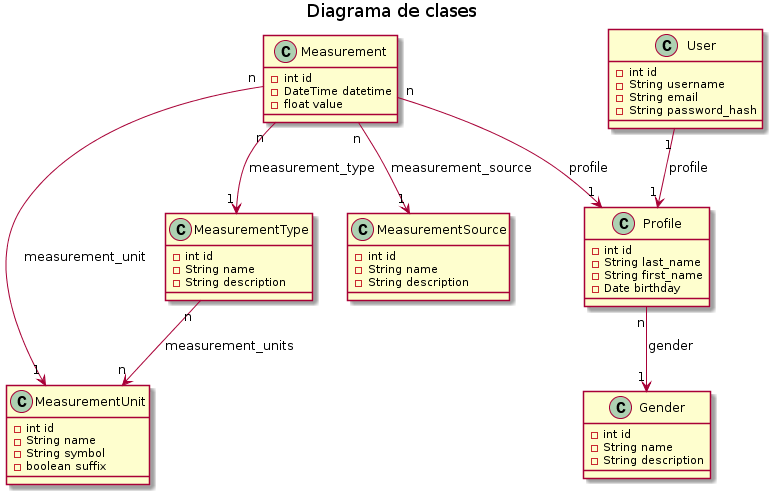
\includegraphics[width=.8\textwidth]{img/3-diagramaClases_relacionTipos}
	\caption{Diagrama de clases donde se puede ver la relación entre el tipo de medición y la unidad}
	\label{relacion_tipo}
\end{figure}


\textbf{ Clase MeasurementType }

Esta clase nos permitirá  nomenclar  los tipos de medidas, hasta el momento hemos contemplado: peso, dimensión corporal (Ej:altura) y glucosa. Existen ciertas medidas que contemplan dos valores, estas serán agregadas en un sprint futuro.

\textbf{Descripción de los atributos}
\begin{itemize}
	\item \textbf{name: }	Nombre del tipo de medición(tipo string).
	\item \textbf{description:} Descripción del tipo de medición (tipo string).
\end{itemize}

\textbf{Dirección del recurso:}
\begin{lstlisting}[language=json,firstnumber=1]
<BASE URL>/measurement_types/{id}
\end{lstlisting}

\textbf{Json generado por la API} 
\begin{lstlisting}[language=json,firstnumber=1]
{
"resource": 
{
"name": "Peso",
"description": "Peso corporal de la persona.",
"id": 1
}
}
\end{lstlisting}

\textbf{ Clase MeasurementUnit }

Esta clase nos permitirá  nomenclar  las unidades de medicion disponible para que el usuario pueda seleccionarlas cdo realice la medición, hasta el momento hemos contemplado: Kilogramo, gramo, miligramos, metro, centimetro y milímetro.

\textbf{Descripción de los atributos}
\begin{itemize}
	\item \textbf{id:	}	Identificador único de la unidad de medición(tipo int).
	\item \textbf{name :	}	Nombre de la unidad de medición ( tipo string).
	\item \textbf{symbol :}		Símbolo de la unidad de medición (tipo string).
	\item \textbf{suffix :}	Variable booleana que indica si el símbolo de la unidad de medición es un sufijo (verdadero) o un prefijo (falso) del valor de la medición (tipo boolean).
\end{itemize}

\textbf{Dirección del recurso}
\begin{lstlisting}[language=json,firstnumber=1]
<BASE URL>/measurement_units/{id}
\end{lstlisting}

\textbf{Json generado por la API} 

\begin{lstlisting}[language=json,firstnumber=1]
{
"resource": 
{
"symbol": "Kg",
"suffix": true,
"name": "Kilogramo",
"id": 1
}
}
\end{lstlisting}



Pero fundamentalmente necesitamos el recurso que nos permite traer las unidades de medidas a partir de un tipo particular de medición, dicho recurso se accede por:
\textbf{Dirección del recurso}
\begin{lstlisting}[language=json,firstnumber=1]
<BASE URL>/measurement_types/{id}/units
\end{lstlisting}
\textbf{Json generado por la API} 

Retorna la lista de unidades de medición relacionadas a un tipo de medición específico.
\begin{lstlisting}[language=json, caption=Json generado por la api, label=unitPeso]

{    "resource": 
[{
"id": 1,
"symbol": "Kg",
"suffix": true,
"name": "Kilogramo"
},
{
"id": 6,
"symbol": "g",
"suffix": true,
"name": "gramo"
}]
}
\end{lstlisting}


\subsection{Pruebas ejecutadas}
A continuación se detalla la situación en la que quedaron las pruebas ejecutadas en los sprint anteriores, luego se desarrollarán las soluciones que se usaron y por última se cambiará el estado de aquellas errores encontrados por \textit{"cerrado"}.
        %
	\begin{itemize}
		\item \textbf{¿Qué fue bien?}
        	\begin{itemize}
				\item        Las cargas y ediciones se llevan a cabo correctamente.
			\end{itemize}

   		\item \textbf{¿Qué se mejoró?}
        	\begin{itemize}
				\item \textbf{Cerrado} Al crear una nueva medición, se mostraba un cartel (alert de javascript) con una fecha, dicho alert fue eliminado.
                \item \textbf{Cerrado} Se encontró un problema con la zona horaria que usa el servidor y la zona horaria del usuario, para solucionarlo hubo q hacer un casteo previo cuando se solicitaba la fecha y hora del usuario para mostrar.
			\end{itemize}

   		\item \textbf{¿Qué se puede mejorar?}
        	\begin{itemize}
		        \item \textbf{Abierto} Solo debería mostrarse las unidades relacionadas al tipo de medición que se ha seleccionado 
				\item \textbf{Abierto} En el futuro se deberá mejorar las validaciones de los datos a la hora de cargar información en los formularios.
        		\item \textbf{Abierto} Se deberá mejorar la manera de seleccionar la fecha y la hora. 
                \item \textbf{Abierto} Deberá realizarse los carteles de advertencia necesarios.
            \end{itemize}
       
	\end{itemize}

\textbf{Mostrar unidades relacionadas al tipo de medición seleccionado}

Para evitar errores humanos fue necesario mostrar sólo las unidades de medida que se encuentran relacionadas a un tipo de medición seleccionada por el usuario, por ejemplo: si selecciona Tipo de medición, ``\textit{Peso}'', como se muestra en la \textbf{Figura \ref{unidad_peso}} el sistema solo debería mostrar las unidades que correspondan a ese tipo de medición y no mostrar metros como una posible unidad igual para el caso de que seleccione la altura  \textbf{Figura \ref{unidad_altura}}.

A nivel de frontEnd fue necesario deshabilitar  la selección de unidades cuando el usuario no ha seleccionado el tipo de medición como se indica en la \textbf{Figura \ref{msj_seleccione_tipo}} y una vez seleccionado se tuvo que solicitar a un recurso de la API las unidades relacionadas al tipo de medición seleccionado como se muestran en las figuras antes citadas.

 
 \begin{figure}[h!]
  \centering
  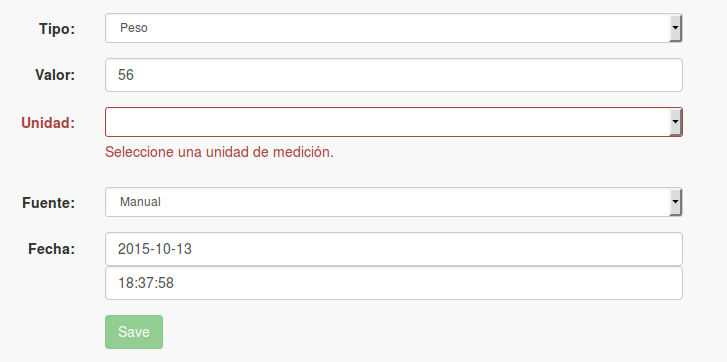
\includegraphics[width=.8\textwidth]{img/3-selecciona_tipo}
  \caption{Mensaje sutil que solicita que se seleccione un tipo de medición }
  \label{msj_seleccione_tipo}
\end{figure}

\begin{figure}[h!]
  \centering
  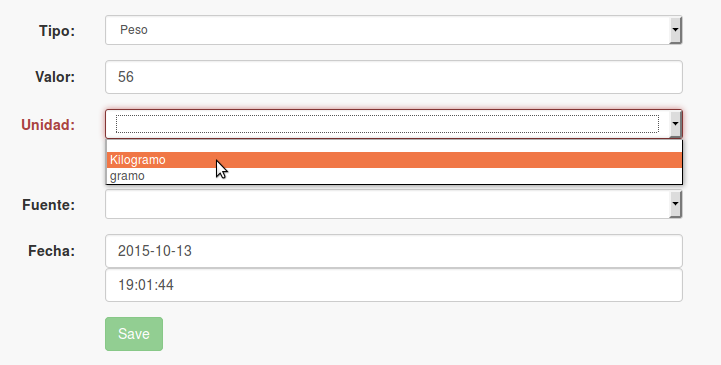
\includegraphics[width=.8\textwidth]{img/3-unidad_peso}
  \caption{Lista de unidades al seleccionar el tipo de unidad ``Peso''}
  \label{unidad_peso}
\end{figure}

 \begin{figure}[h!]
  \centering
  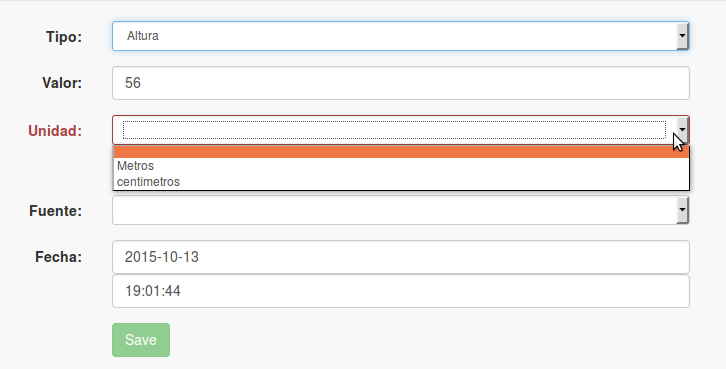
\includegraphics[width=.8\textwidth]{img/3-unidad_altura}
  \caption{Lista de unidades al seleccionar el tipo de unidad ``Altura''}
  \label{unidad_altura}
\end{figure}


El diagrama de clases, las relaciones y los recursos de la API necesarios para poder establecer esta relación se detallan en el apartado \ref{3-clases_involucradas}

\textbf{Carteles de alertas}

Luego de ejecutar las pruebas se detectó que para mejorar la experiencia del usuario es necesario añadir mensajes de avisos, como se muestra en la \textbf{Figura \ref{msj_presiona_no_escribe} y Figura \ref{msj_escribir_borrar}} indicando al usuario situaciones importantes como las que indican ausencia de información importante en el formulario, además el botón para enviar el formulario se mantiene deshabilitado hasta que se haya completado los datos obligatorios (que en este caso serían todos) del formulario.


 \begin{figure}[h!]
  \centering
  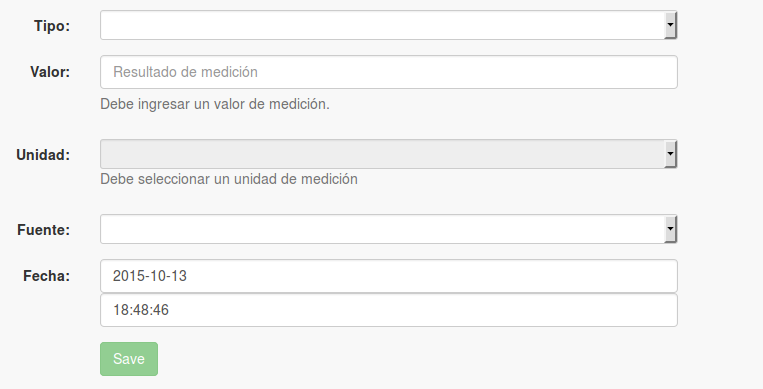
\includegraphics[width=.8\textwidth]{img/3-presiona_no_escribe}
  \caption{Mensaje sutil que aparece  si se ha presionado el campo y no se ha escrito nada}
  \label{msj_presiona_no_escribe}
\end{figure}

\begin{figure}[h!]
  \centering
  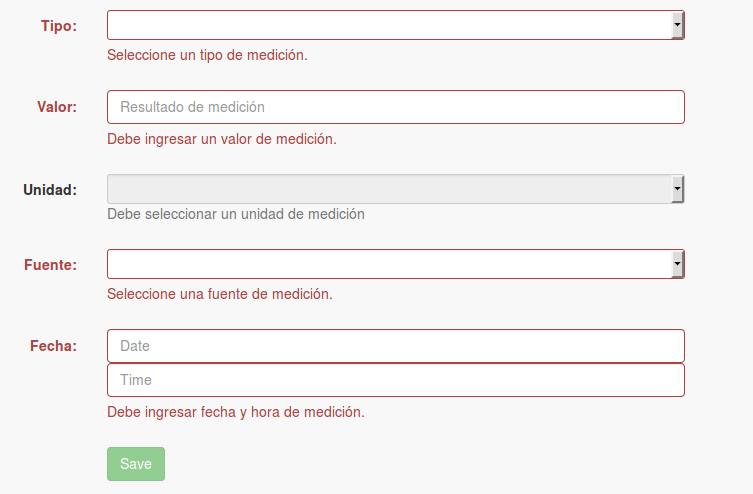
\includegraphics[width=.8\textwidth]{img/3-escribir_borrar}
  \caption{Mensaje vistoso que aparece luego de borrar lo escrito}
  \label{msj_escribir_borrar}
\end{figure}

\clearpage

\begin{lstlisting}[language=JavaScript, caption= recurso que solicita las unidades de un tipo de medición específico, label=type_unit]

 angular.module('saludWebApp')                                                   
 .factory('MeasurementTypeUnit', function (global, $resource) {                  
     // URL of specific API resource                                             
     var url=global.getApiUrl()+'/measurement_types/:id_type/units';             
                                                                                 
     return $resource( url,                                                      
         { id_type: '@_id_type' },                                                        
         { query:{method:'GET',isArray:false},                                   
           update: {method: 'PUT'}                                               
         });                                                                     
}); 
                                                                            
\end{lstlisting}



\textbf{Variable de acceso a la API global}

Fue necesario añadir  un servicio para manejar la dirección global de la API, dicho servicio se detalla en \textbf{Listing \ref{direccion_global}}
\begin{lstlisting}[language=JavaScript, caption= Servicio de la dirección global de la API, label=direccion_global]
'use strict';                                                                   
                                                                                
/**                                                                             
 * @ngdoc service                                                               
 * @name saludWebApp.global                                                     
 * @description                                                                 
 * # global                                                                     
 * Factory in the saludWebApp.                                                  
 */                                                                             
angular.module('saludWebApp')                                                   
  .factory('global', function () {                                              
    // Service logic                                                               
                                                                                
    // URL of yesdoc API                                                           
    var _api_url='https://yesdoc-api.herokuapp.com';                               
                                                                                   
    // Public methods                                                              
    return {                                                                       
      getApiUrl: function () {                                                     
        return _api_url;                                                           
      }                                                                            
    };                                                                             
  });                                                                              
~                                                                            
\end{lstlisting}


\clearpage


\subsection{Estado final de pruebas}

	\begin{itemize}
		\item \textbf{¿Qué fue bien?}
        	\begin{itemize}
				\item        Las cargas y ediciones se llevan a cabo correctamente.
			\end{itemize}

   		\item \textbf{¿Qué se mejoró?}
        	\begin{itemize}
				\item \textbf{Cerrado} Al crear una nueva medición, se mostraba un cartel (alert de javascript) con una fecha, dicho alert fue eliminado.
                \item \textbf{Cerrado} Se encontró un problema con la zona horaria que usa el servidor y la zona horaria del usuario, para solucionarlo hubo q hacer un casteo previo cuando se solicitaba la fecha y hora del usuario para mostrar.
			\end{itemize}

        	\begin{itemize}
		        \item \textbf{Cerrad0o} Solo debería mostrarse las unidades relacionadas al tipo de medición que se ha seleccionado 
				\item \textbf{Cerrado} En el futuro se deberá mejorar las validaciones de los datos a la hora de cargar información en los formularios.
        		\item \textbf{Cerrado} Se deberá mejorar la manera de seleccionar la fecha y la hora. 
                \item \textbf{Cerrado} Deberá realizarse los carteles de advertencia necesarios.
            \end{itemize}
       
	\end{itemize}
%%%%%%%%%%%%%%%%%%%%%%%%%%%%%%%%%%%%%%%%%%%%%%%%      FIN SPRINT 3  %%%%%%%%%%%%%%%%%%%%%%%%%%%%%%%%%%%%%%%%%%%%%%%%%%%%%%%%%%%%%%%%%%%%
\section{Sprint 4: }%mostrar gráficas -validaciones
\subsection{Planificación}

\textbf{Inicio: }Martes 17 de julio del 2015 

\textbf{Fin:} Martes 11 de Septiembre del 2015

\begin{figure}[h!]
  \centering
  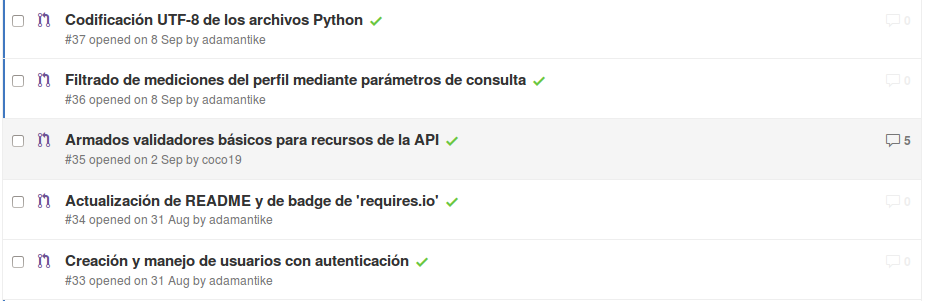
\includegraphics[width=.8\textwidth]{img/4-PR_back}
  \caption{Pull request realizados por el back end en el sprint  34}
  \label{4-PR_back}
\end{figure}
\begin{figure}[h!]
  \centering
  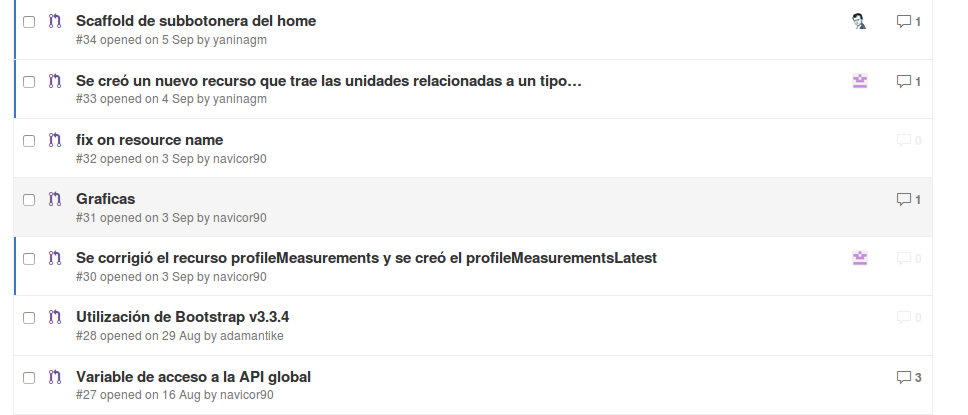
\includegraphics[width=.8\textwidth]{img/4-PR_front}
  \caption{Pull request realizados por el front end en el sprint  3}
  \label{4-PR_front}
\end{figure}

	{\scriptsize
	\begin{center} %sidewaystable
	\centering
	%\begin{adjustbox}{max width=\textheight}
    \resizebox{\textwidth}{!}
    {
	\begin{tabular}{|l|l|p{5cm}|l|l|}
	    \hline
	        \textbf{Area a cargo} &
	        \textbf{Responsable} &        
	        \textbf{Tarea} &
	        \textbf{US} &
            \textbf{Tiempo}\\
   		\hline
       
	    Back-end& Franco Canizo & Agrega a la estructura de la API paquete para validadores generales.  & US-\ref{resumenInfo} \& US-\ref{infoSalud} & 8hs\\ \hline
	    Back-end& Franco Canizo & Creación de validadores para números enteros positivos, fecha, fecha-hora, fecha-hora previa, string con\/sin números  & US-\ref{resumenInfo} \& US-\ref{infoSalud} &8hs\\ \hline
	    Back-end& Michael Manganiello & filtrado de mediciones en base al tipo, fuente y unidad de medición & US-\ref{resumenInfo} \& US-\ref{infoSalud}&9hs \\ \hline
	    Back-end& Michael Manganiello & Corrección error de comparación de fechas con información de zona horaria y fechas sin esa información & US-\ref{resumenInfo} \& US-\ref{infoSalud} &8hs\\ \hline
	    Back-end& Michael Manganiello & Simplificación del parseo de argumentos date y datetime & US-\ref{resumenInfo} \& US-\ref{infoSalud} &5hs \\ \hline        
   	    Front-end& Ivan Terreno & Capacitación en D3 & \textbf{US-17} \& \textbf{US-15}&18hs\\ \hline
   	    Front-end& Ivan Terreno & Generación de gráficas & \textbf{US-17} \& \textbf{US-15}&10hs\\ \hline        
	    \end{tabular}
        }
	    %\end{adjustbox}
    	\end{center}
	}


\subsection{Descripción}
%%Descripción de Franco de validadores

Además se describirán las tareas realizadas para realizar las gráficas de las distintas mediciones

\subsection{User Stories relacionados}
La \textbf{Tabla \ref{US-Sprint3} } indicará las características de cada user story para guiarnos en el desarrollo del sprint.

\begin{table}[h]
    \label{US-Sprint3}
	%\resizebox{\textwidth}{!}{
    \centering
	\begin{tabular}{|l|p{9cm}|}
	\hline
        \multicolumn{1}{|c|}{\textbf{ID}} &
        \multicolumn{1}{|c|}{\textbf{Enunciado de la historia}} \\          
    \hline
        \textbf{US-2 } & Como paciente, quiero añadir al sistema los estudios realizados para evitar posibles perdidas.\\
     \hline 
        \textbf{US-5 } & Como paciente quiero que los sistemas de salud existentes puedan cargar sus resultados directamente en mi carpeta de salud para centralizar mi información. \\
      \hline 
        \textbf{US-7} & Como paciente quiero categorizar mis estudios por rama de medicina, para lograr una mejor organización y navegabilidad en el sistema. \\
       \hline 
        \textbf{US-8} & Como laboratorio, quiero cargar información de un paciente en su cuenta para ahorrarle las molestias de volver. \\
        \\
    \hline 
	    \textbf{US-17} &   Como paciente quiero ver gráficas que resuman mi información en particular para poder ver mis cambios a lo largo de la historia.\\
    \hline        
        \textbf{US-15} & Como médico quiero ver gráficas que resuman la información de un paciente para poder ver sus cambios a lo largo de la historia y así apoyar la toma de decisiones y el diagnóstico.\\
    \hline
    \end{tabular}
%     }

\end{table}

\subsection{ Modelo funcional.} 
Se describirán las funciones usando como marco de apoyo el sprint Backlog,
además se armará el diagrama de casos de uso del presente Sprint [Figura 44] que
irá creciendo medida se vaya avanzando en el proyecto.

\begin{comment}
	Faltaría diagrama de casos de uso para esta parte.
\end{comment}


\begin{comment}
\subsubsection{Creación de página de mediciones}
\end{comment}

\subsubsection{Validadores}
Del lado del backend el trabajo consistión en la definición de validadores usados para controlar errores y, de ser posible, sanear los datos que envían las representaciones a los recursos. Lo que se hizo es definir en un paquete una serie de validadores generales usados en el paquete parsers en common. Cómo podemos apreciar en la definición del parser usado por el reurso de mediciones:

\begin{lstlisting}[language=Python]
parser = reqparse.RequestParser()
parser.add_argument('datetime', type=is_valid_previous_datetime, required=True)
parser.add_argument('value', type=float, required=True)
parser.add_argument('analysis_id', type=is_valid_id, required=True)
parser.add_argument('profile_id', type=is_valid_id, required=True)
parser.add_argument('measurement_source_id', type=is_valid_id)
parser.add_argument('measurement_type_id', type=is_valid_id, required=True)
parser.add_argument('measurement_unit_id', type=is_valid_id, required=True)
\end{lstlisting}

Se define en el argumento type el llamado a una función is\_valid\_previous\_datetime, está función está definida en el paquete validators en el archivo generic validators.

\begin{lstlisting}[language=Python]
    datetime_var = is_valid_datetime(var)
    if datetime_var.year < 1900:
        raise ValueError("La fecha y hora ingresada no puede ser anterior al anio 1900.")
    elif datetime_var > datetime.utcnow():
        raise ValueError("La fecha y hora ingresada no debe ser posterior a la fecha y hora actual.")
    else:
        return datetime_var
\end{lstlisting}

Este a su vez llama al validador is\_valid\_datetime para controlar que el dato ``datetime'' tenga un valor de fecha-hora correcto. Si el validador no encuentra error devuelve la fecha-hora, en caso contrario lanza un error.
En este parser también se define un método para controlar que el id recibido es valido, por el momento lo que hace este es controlar que el id recibido sea positivo.
\begin{comment}
	Se podría poner como cosas a mejorar la validación de id.
\end{comment}

\subsubsection{Filtrado de mediciones}
El backend identifica como útil la definición de un recurso que permita devolver medidas de un perfil específico filtradas según tipo, fuente y unidad de medida. Para esto se agregó un recurso \/profile\/id\/measurements en el archivo principal de la aplicación y un recurso que define un método get para responder a una solicitud HTTP con operador GET. El mismo utiliza los datos recibidos en el ``query string'' de la URL para determinar según que tipo, fuente o unidad de medida debe filtrar. El recurso en sí no se encarga del filtrado sino que toma los datos verificados por el parse, obtiene los datos del query string y pasa estos datos a un método auxiliar definido en el archivo measurement del paquete persistence de la API ``get\_by\_profile'' el cual devuelve todas las instancias existentes de medición, asociadas a un perfil específico, ordenadas por fecha y hora de la medición, y filtradas por fuente, tipo y unidad de medición. Una vez recibida la respuesta arma el response con el código de estado correspondiente y en el cuerpo los datos resultantes serializados de acuerdo a la representación utilizada.



\subsubsection{gráficas}
Para las gráficas se utilizo D3, fue necesario añadir código javascript, el cual fue añadido con grunt
\subsection{Salidas del sistema}
El resultado de la implementación del código necesario para mostrar las gráficas del peso se puede ver en la \textbf{[Figura \ref{5-grafica_medicion}]}, 


\begin{figure}[h!]
  \centering
  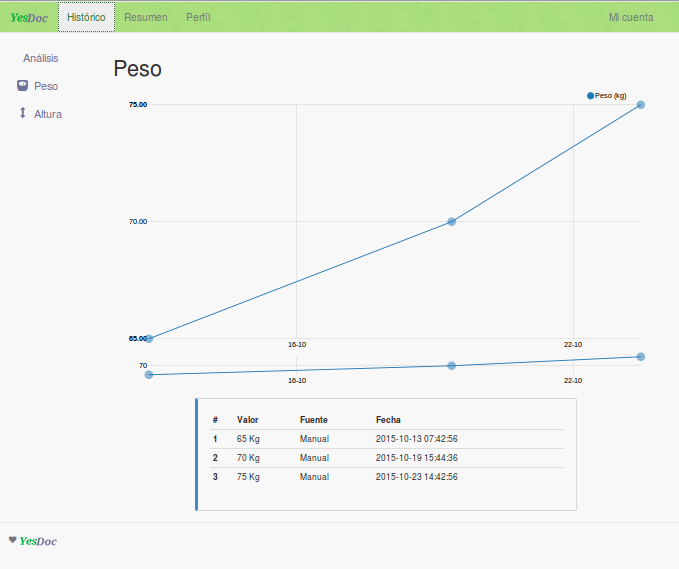
\includegraphics[width=.8\textwidth]{img/5-grafica_medicion}
  \caption{vista generada para una medición en particular}
  \label{5-grafica_medicion}
\end{figure}


\begin{comment}
	Faltaría agregar algunas pruebas con curl y algo de código.
    Poner que se desarrollo para pasar datos específicos para que el front-end presente datos resumidos cuando estos son muchos y complejos??
\end{comment}

\subsection{Criterios de aceptación}

\begin{center}
\begin{longtable}{|p{0.5cm}|p{4cm}|p{4cm}|p{5cm}|}
\hline \hline \rowcolor[gray]{0.9}
	\multicolumn{4}{||c|}{\textbf{Criterio de aceptación}} \\
    \hline  \rowcolor[gray]{0.9}
        \textbf{Id} &
        \textbf{Contexto} &
        \textbf{Evento}&
        \textbf{Resultado} \\
    \hline
1&En caso de que se envíe como id un valor menor o igual a 0 en cualquier representación  de una solicitud & Al ejecutar el método post, get, delete o put correspondiente del recurso & El sistema devolverá un json con el mensaje de error por entero no positivo y el código de error 400 \\ \hline
	\hline
2&En caso de que se indique una fecha cuyo año sea menor a 1900 & al ejecutar el validador is\_valid\_previous\_date del argumento  & El sistema devolverá un json con el mensaje de error correspondiente a una fecha previa no permitida y el código de estado 400 \\ 		\hline
	\hline
3&En caso de que se indique en la solicitud una fecha-hora con formato invalida & Al ejecutar el validador is\_valid\_datetime  & El sistema devolverá un json con el mensaje de error correspondiente a una fecha hora con formato inválido y el código de estado 400\\ \hline
    \hline
4&En caso de que no exista un usuario registrado con el id indicado & al ejecutar el método get\/put del recurso \/users\/id  & El sistema devolverá un json con un mensaje de error y un código de error 404 \\ \hline
	\hline
5&En caso de que no exista un perfil registrado con el id indicado & al ejecutar el método get del recurso \/profile\/id\/measurements  & El sistema devolverá un json con un mensaje de error por no encontrar la instancia correspondiente \\ \hline

  \end{longtable}
\end{center}

\begin{comment}
	Cuando paso un entero no positivo no responde con error sino que query or get 404 no encuentra el registro.
    El método get_latest_by_profile es del sprint2 cierto?
\end{comment}

\subsection{Pruebas ejecutadas}
A continuación se detalla la situación en la que quedaron las pruebas ejecutadas en los sprint anteriores, luego se desarrollarán las soluciones que se usaron y por última se cambiará el estado de aquellas errores encontrados por \textit{"cerrado"}.
        %
	\begin{itemize}
		\item \textbf{¿Qué fue bien?}
        	\begin{itemize}
				\item        Las cargas y ediciones se llevan a cabo correctamente.
			\end{itemize}

   		\item \textbf{¿Qué se mejoró?}
        	\begin{itemize}
				\item \textbf{Cerrado} Al crear una nueva medición, se mostraba un cartel (alert de javascript) con una fecha, dicho alert fue eliminado.
                \item \textbf{Cerrado} Se encontró un problema con la zona horaria que usa el servidor y la zona horaria del usuario, para solucionarlo hubo q hacer un casteo previo cuando se solicitaba la fecha y hora del usuario para mostrar.
			\end{itemize}

   		\item \textbf{¿Qué se puede mejorar?}
        	\begin{itemize}
		        \item \textbf{Abierto} Solo debería mostrarse las unidades relacionadas al tipo de medición que se ha seleccionado 
				\item \textbf{Abierto} En el futuro se deberá mejorar las validaciones de los datos a la hora de cargar información en los formularios.
        		\item \textbf{Abierto} Se deberá mejorar la manera de seleccionar la fecha y la hora. 
                \item \textbf{Abierto} Deberá realizarse los carteles de advertencia necesarios.
            \end{itemize}
       
	\end{itemize}



\subsection{Estado final de pruebas}

	\begin{itemize}
		\item \textbf{¿Qué fue bien?}
        	\begin{itemize}
				\item        Las validaciones.
			\end{itemize}
            
		\item \textbf{¿Qué fue mal?}
        	\begin{itemize}
				\item        La librería que se utilizó al principio ``lvd3'' era de muy bajo nivel, por ello tuvo q cambiarse a D3 que es de más alto nivel. 
			\end{itemize}
            
   		\item \textbf{¿Qué se mejoró?}
        	\begin{itemize}
            	\item \textbf{Cerrado} Mal rendimiento de D3, mejorado usando código de la libreria lvd3
            	\item \textbf{Cerrado} Función de maximizar
                \item \textbf{Cerrado} Facilitar el pasaje del scope al controlador
                \item \textbf{Cerrado} Se encontró un problema con la zona horaria que usa el servidor y la zona horaria del usuario, para solucionarlo hubo q hacer un casteo previo cuando se solicitaba la fecha y hora del usuario para mostrar.
			\end{itemize}
       
	\end{itemize}

%%%%%%%%%%%%%%%%%%%%%%%%%%%%%%%%%%%%%%%%%%%%%%%%%%%%%%%%%%%%%%%%%%%%%%      FIN SPRINT 4  %%%%%%%%%%%%%%%%%%%%%%%%%%%%%%%%%%%%%%%%%%%%%%%%%%%%%%%%%%%%%%%%%%%%%%%%%%%%%%%%%%%%%%%%%%%

\section{Sprint 5}%Autenticación
\subsection{Planificación}

\textbf{Inicio: } 10 de Septiembre del 2015

\textbf{Fin:} 27 de Septiembre del 2015 



\subsection{Descripción}

Este sprint tiene por objetivo definir un proceso de autenticación del usuario para con la API, sin importar el perfil del mismo, que garantice un nivel de seguridad adecuado para tranquilidad en el uso de la aplicación por parte de los interesados. 

\subsection{User Stories relacionados}
La \textbf{Tabla \ref{US-Sprint4} } indicará las características de cada user story para guiarnos en el desarrollo del sprint.
\begin{comment}
	como usuario quiero contar con un acceso único y privado a mi información. Agregaría este user story, habría que ver la traza con el documento de diseño para que queden balanceados.
\end{comment}
\begin{table}[h]
    \label{US-Sprint4}
	%\resizebox{\textwidth}{!}{
    \centering
	\begin{tabular}{|l|p{9cm}|}
	\hline
        \multicolumn{1}{|c|}{\textbf{ID}} &
        \multicolumn{1}{|c|}{\textbf{Enunciado de la historia}} \\          
    \hline
        \textbf{US-11 } & Como paciente, quiero modificar los permisos de visualización de mis datos con respecto a cada uno de los integrantes de grupo familiar para tener un control total sobre mi privacidad. \\
     \hline 
     \hline
        \textbf{US-21 } & Como usuario quiero contar con un acceso único y privado a mi información. \\
     \hline 
     
    \end{tabular}
%     }

\end{table}
\subsection{Modelo de datos}
El Diagrama propio de este sprint se puede ver en la \textbf{Figura\ref{4-clase_autenticacion}}, allí se indican exactamente las clases que se usarán en este sprint y que serán detalladas con detenimiento en el presente documento. 

\begin{figure}[h]
        \centering
        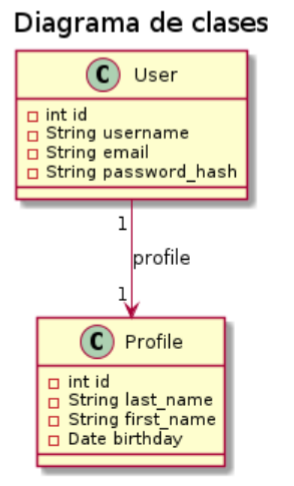
\includegraphics[width=0.5\textwidth]{img/clases_auth}
        \caption{Diagrama de clases autenticación.}
		\label{4-clase_autenticacion}
    \end{figure}

\subsection{ Modelo funcional.} 
Se define el diagrama de casos de uso del presente Sprint \textbf{[Figura \ref{4-cu_autenticacion}]}.

    \begin{figure}[h]
        \centering
        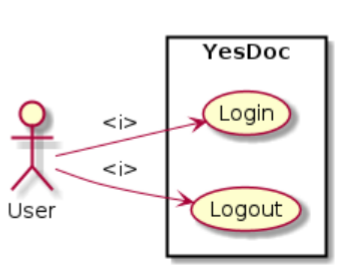
\includegraphics[width=0.5\textwidth]{img/cu_autenticacion}
        \caption{Casos de uso autenticación}
		\label{4-cu_autenticacion}
    \end{figure}

	{\scriptsize
	\begin{center} %sidewaystable
	\centering
	%\begin{adjustbox}{max width=\textheight}
    \resizebox{\textwidth}{!}{
	\begin{tabular}{|l|l|l|l|}
	    \hline
	        \textbf{Area a cargo} &
	        \textbf{Responsable} &        
	        \textbf{Tarea} &
	        \textbf{US} \\
	    \hline
	    Backend& Michael Manganiello & Generación del modelo User y relación del mismo con el modelo Profile.  & US-\ref{resumenInfo} \& US-\ref{infoSalud} \\ \hline
        \hline
	    Backend& Michael Manganiello & Generación del recurso relacionado con el modelo User y los métodos post y get que manejan los operadores HTTP correspondientes.  & US-\ref{resumenInfo} \& US-\ref{infoSalud} \\ \hline
        \hline
	    Backend& Michael Manganiello & Generación del recurso para obtener un token para un usuario autenticado.  & US-\ref{resumenInfo} \& US-\ref{infoSalud} \\ \hline

	    \end{tabular}
        }
	    %\end{adjustbox}
    	\end{center}
	}
    
\subsubsection{Definición de modelos}
La definición del modelo User es bastante compleja ya que define métodos para tomar la password  y guardarla como un hash, a su vez, puede recibir passwords encriptadas y desencriptarlas. Por otro lado, define métodos para la generación y verificación del token asignado al usuario. Por último, define una relación uno a uno con el modelo Profile.

\subsubsection{Recursos}
El desafío en cuanto a la definición de recursos radica en que según lo que establece REST, la restricción de que la API debe ser stateless invalida la posibilidad de usar sesiones para que la API sea escalable, es por esto que definimos una solución que se presenta en un punto gris entre puristas de REST y quienes realmente no hacen REST. La solución consiste en generar un token para el usuario autenticado el cual se almacena en las cookies y es usado en cada solicitud para autenticar al usuario. Por esto se definen recursos para dar de alta al usuario y para entregarle un token.

	\begin{lstlisting}[language=Python]
	api.add_resource(UserView, '/users/<int:id>')
	api.add_resource(UserList, '/users')
	api.add_resource(Token, '/token')
	api.add_resource(MyUserView, '/my/user')
	\end{lstlisting}

\subsection {Salidas del Sistema}

\begin{enumerate}
	\item \textbf{Solicitud post al recurso del perfil}
    
	Para crear un usuario debe existir un perfil creado, para esto usamos el recurso ``\/profiles'' a través del método POST y pasando como argumento los datos first\_name, last\_name, birthday y gender\_id.
    \item \textbf{Solicitud post al recurso del user}
    
    Realizamos ahora una solicitud HTTP, con método post utilizando curl al recurso del usuario usando el id del perfil creado previamente:

\begin{verbatim}
curl -i http://localhost:5000/users -H "Content-Type: 
application/json" -X POST -d '{"username":"akathy", 
"email":"kathy@gmail.com", "password":"kathy1234", 
"profile_id":"2"}'
\end{verbatim}
    
    Obtenemos la siguiente respuesta de la API, con un código 201.
    
\begin{lstlisting}[language=json]
HTTP/1.0 201 CREATED
Content-Type: application/json
Content-Length: 425
Server: Werkzeug/0.10.4 Python/2.7.6
Date: Tue, 20 Oct 2015 05:21:37 GMT

{
    "resource": {
        "email": "kathy@gmail.com", 
        "id": 2, 
        "profile": {
            "birthday": "1989-06-17", 
            "first_name": "Katherina", 
            "gender": {
                "description": "female gender", 
                "id": 2, 
                "name": "female"
            }, 
            "id": 2, 
            "last_name": "Aguirre"
        }, 
        "username": "akathy"
    }
}
\end{lstlisting}

    \item \textbf{Solicitud post al recurso token usando user y password}
    
    Luego con este usuario y contraseña solicitamos un token al recurso correspondiente:

\begin{verbatim}
curl -u akathy:kathy1234 http://localhost:5000/token
\end{verbatim}
   
   Obtenemos así el token que debe ser almacenado en las cookies, tendrá una duración de 10 minutos y será utilizado en cada solicitud para autenticación.
   
\begin{lstlisting}[language=json]
{
    "resource": {
        "duration": 600, 
        "token": "eyJhbGciOiJIUzI1NiIsImV4cCI6MTQ0NTMxOTM3MCwiaWF0IjoxNDQ1MzE4NzcwfQ.eyJpZCI6Mn0.2eZRjbMq9tg4GykJx8EU-Ux4ZoyUW6WnBlADsvnpQvE"
    }
}
\end{lstlisting}

\end{enumerate}

\subsection{Criterios de aceptación}

\begin{center}
\begin{longtable}{|p{0.5cm}|p{4cm}|p{4cm}|p{5cm}|}
\hline \hline \rowcolor[gray]{0.9}
	\multicolumn{4}{||c|}{\textbf{Criterio de aceptación}} \\
    \hline  \rowcolor[gray]{0.9}
        \textbf{Id} &
        \textbf{Contexto} &
        \textbf{Evento}&
        \textbf{Resultado} \\
    \hline
1&En caso de que exista un usuario registrado con el mismo username & al ejecutar el método post del recurso \/users  & El sistema devolverá un json vacío y un código de error 400 \\ \hline
	\hline
2&En caso de que exista al menos un usuario registrado & al ejecutar el método get del recurso \/users  & El sistema devolverá una lista de json con los datos de los users registrados \\ 		\hline
	\hline
3&En caso de que exista un usuario registrado con el mismo username & al ejecutar el método post del recurso \/users  & El sistema devolverá un json vacío y un código de error 400 \\ \hline
    \hline
4&En caso de que no exista un usuario registrado con el id indicado & al ejecutar el método get\/put del recurso \/users\/id  & El sistema devolverá un json con un mensaje de error y un código de error 404 \\ \hline

  \end{longtable}
\end{center}

\begin{comment}
	Cuando devolvería 401 el recurso del token.
\end{comment}

\subsection{Casos de prueba}

\subsubsection{Pruebas  de  integración  entre módulos del Sistema}

\subsubsection{ Pruebas de carga}

\subsubsection{ Pruebas de seguridad por niveles de usuarios}


\subsection{Pruebas ejecutadas}
Aqui se realizará una conclusión general de lo que se descubrió en las pruebas.
        %
	\begin{itemize}
		\item \textbf{¿Que fue bien?}
        	\begin{itemize}
				\item        Las cargas y ediciones se llevan a cabo correctamente.
			\end{itemize}

   		\item \textbf{¿Que se mejoró?}
        	\begin{itemize}
                \item \textbf{Cerrado} problema
			\end{itemize}

   		\item \textbf{¿Que se puede mejorar?}
        	\begin{itemize}
		        \item \textbf{Abierto} En el futuro se deberá mejorar ...
            \end{itemize}
        

	\end{itemize}

%%%%%%%%%%%%%%%%%%%%%%%%%%%%%%%%%%%%%%%%%%%%%%%%%%%%%%%%%%%%%%%%    FIN SPRINT 5    %%%%%%%%%%%%%%%%%%%%%%%%%%%%%%%%%%%%%%%%%%%%%%%%%%%%%%%%%%%%%%%




\section{Sprint 6} % MOSTRAR, CARGAR Y EDITAR ANÁLISIS
\subsection{Planificación}

\textbf{Inicio: }Martes 11 de setiembre del 2015 

\textbf{Fin:} Martes 17 de octubre del 2015

\begin{figure}[h!]
  \centering
  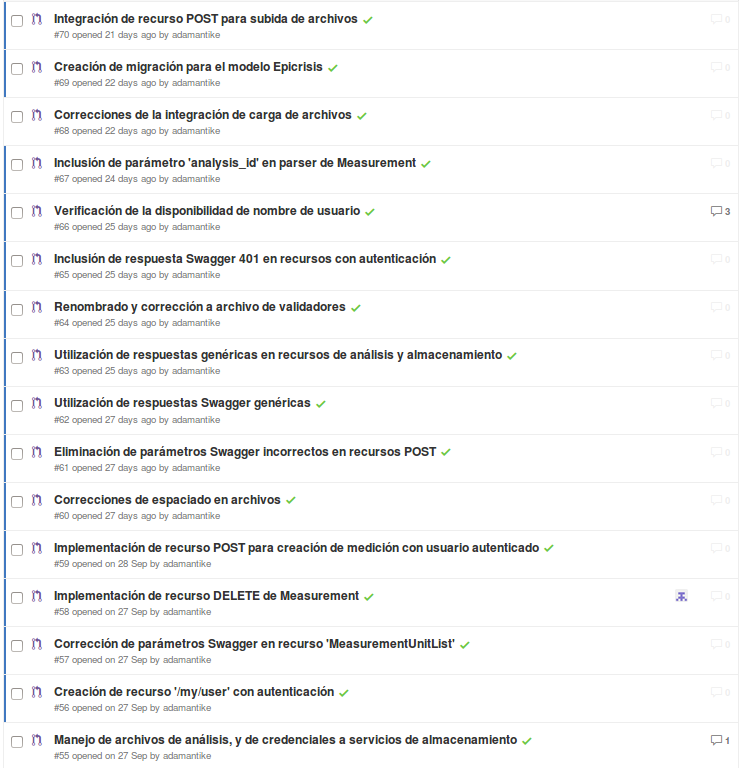
\includegraphics[width=.8\textwidth]{img/6-PR_1}
  \caption{Pull request realizados en el sprint  6}
  \label{6-PR_1}
\end{figure}

\begin{figure}[h!]
	\centering
	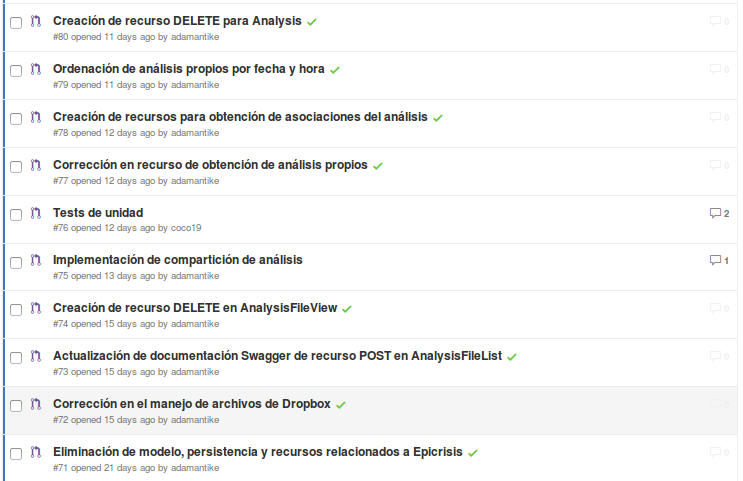
\includegraphics[width=.8\textwidth]{img/6-PR_2}
	\caption{Pull request realizados en el sprint 6}
	\label{6-PR_1}
\end{figure}
\clearpage



{\scriptsize
	\begin{center} %sidewaystable
		\centering
		%\begin{adjustbox}{max width=\textheight}
		\resizebox{\textwidth}{!}{
			\begin{tabular}{|l|l|l|l|l|}
				\hline
				\textbf{Area a cargo} &
				\textbf{Responsable} &        
				\textbf{Tarea} &
				\textbf{US} &
				\textbf{tiempo dedicado}\\
				\hline
				Front-end& Ivan Terreno & Diseño de Interface de epicrisis & \textbf{US 2} & 8 hs\\ \hline
				Front-end& Ivan Terreno & Enlazado de interfaces ya existentes de mediciones con la nueva interfaz & \textbf{US 2} & 3hs \\ \hline
				Front-end& Ivan Terreno & Creación de los recursos que consumirán la información de la API & \textbf{US 2}\& US-\ref{infoSalud} &3 hs\\ \hline
				Front-end& Ivan Terreno & Búsqueda de iconos representativos& US-\ref{resumenInfo} \& \textbf{US 2}& 1hs\\ \hline
				Front-end& Ivan Terreno & Detección de tipo de archivo& US-\ref{resumenInfo} \& \textbf{US 2} & 5hs\\ \hline        
				Front-end& Ivan Terreno &  Carga de archivos,por POST & US-\ref{resumenInfo} \& \textbf{US 2} & 4hs\\ \hline        
				Front-end& Ivan Terreno &  funcionalidad de editar y ver archivos y análisis & US-\ref{resumenInfo} \& \textbf{US 2} & 6hs\\ \hline        
				
			\end{tabular}
		}
		%\end{adjustbox}
	\end{center}
}


\subsection{Descripción}
%navbar responsive
A partir de las funcionalidades ya existentes de carga de medición, se va a crear un análisis consistente y representativo de un análisis de la vida real.

En este sprint se le permitirá al usuario poder cargar las imágenes y las mediciones correspondientes a un mismo análisis, indicando la fecha y hora en la que fue realizado. Esta funcionalidad es muy importante ya que refleja el análisis que el paciente se realiza y le permitirá al médico poder contrastar la validez de las mediciones con un análisis certificado.


Otra funcionalidad importante a desarrollar son las vistas necesarias para mostrar los análisis y el contenido del mismo

\subsection{User Stories relacionados}
La  \ref{sprint-6} indicará las características de cada user story para guiarnos en el desarrollo del sprint.

\begin{table}[h]

	%\resizebox{\textwidth}{!}{
    \centering
	\begin{tabular}{|l|p{9cm}|}
	\hline
        \multicolumn{1}{|c|}{\textbf{ID}} &
        \multicolumn{1}{|c|}{\textbf{Enunciado de la historia}} \\          
    \hline
        \textbf{US-2 } & Como paciente, quiero añadir al sistema los estudios realizados para evitar posibles perdidas.\\
     \hline 
        \textbf{US-5 } & Como paciente quiero que los sistemas de salud existentes puedan cargar sus resultados directamente en mi carpeta de salud para centralizar mi información. \\
      \hline 
        \textbf{US-7} & Como paciente quiero categorizar mis estudios por rama de medicina, para lograr una mejor organización y navegabilidad en el sistema. \\
       \hline 
        \textbf{US-8} & Como laboratorio, quiero cargar información de un paciente en su cuenta para ahorrarle las molestias de volver. \\
        \\
    \hline 

    \end{tabular}
%     }
    \label{sprint-6}
\end{table}

\subsection{ Modelo funcional.} %Diagrama de clases
Se describirán las funciones usando como marco de apoyo el sprint Backlog, además se armará el diagrama de casos de uso del presente Sprint \textbf{[Figura \ref{6-cu}]} acompañado de los casos de uso que se obtuvieron como resultado de los sprint anteriores



\begin{figure}[h]
	\centering
	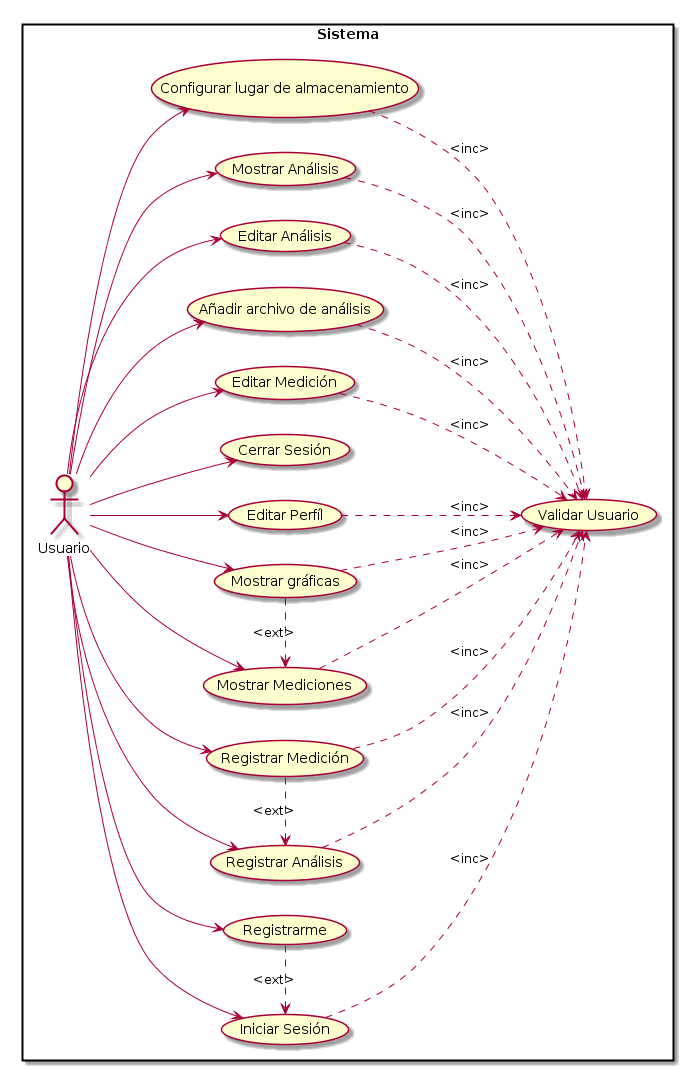
\includegraphics[width=0.6\textwidth]{img/6-cu}
	\caption{formulario de edición de perfil}
	\label{6-cu}
\end{figure}




\subsection{Modelo de datos}
El Diagrama propio de este sprint se puede ver en la \textbf{Figura \ref{5-diagramaClases}}, allí se indican exactamente las clases que se usarán en este sprint, en este documento se detallarán las clases que se han añadido al sprint 2 de mediciones descripto con anterioridad.



    \begin{figure}[h]
        \centering
        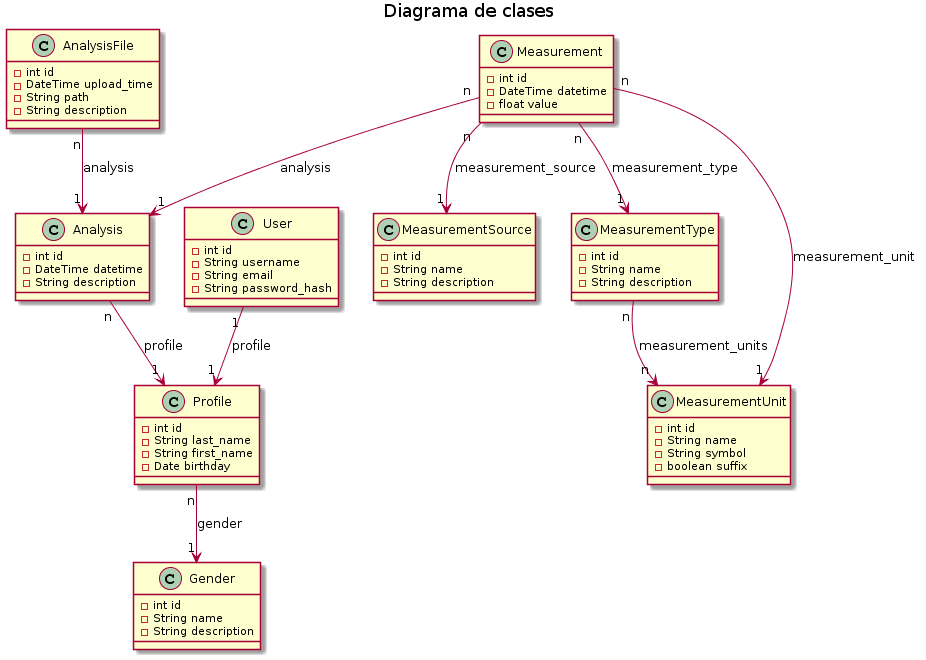
\includegraphics[width=0.8\textwidth]{img/5-diagramaClases}
        \caption{Diagrama de clases referido a la carga de análisis}
		\label{5-diagramaClases}
    \end{figure}

\clearpage

\subsubsection{Analysis}
Como se comentó anteriormente las mediciones se pueden cargar solas e independientes, pero para aquellos casos en que se desee cargar un análisis o una o varias mediciones que posean una imagen asociada se le permite al usuario crear un análisis, el cual estará asociado a uno o mas mediciones y uno o mas imágenes.

La API ofrece 3 métodos \textbf{``POST'',``PUT'' y ``GET''}


\textbf{Descripción de los atributos}
\begin{itemize}
	\item \textbf{description:} Descripción del análisis.
	\item \textbf{datetime: }	Fecha y hora del análisis.	
	\item \textbf{profile\_id: } Identificador único del perfil asociado.
\end{itemize}

\textbf{Dirección del recurso:}
\begin{lstlisting}[language=json,firstnumber=1]
<BASE URL>/analysis
\end{lstlisting}



























































\clearpage
\subsection {Salidas del Sistema - Incrementos}

Luego de finalizado este user story se obtendrán 5 pantallas que se detallarán a continuación:
\begin{enumerate}
	\item \textbf{Vista para acceder a carga de nueva medición}: \textbf{[Figura \ref{5-boton_nuevo_analisis}]} En la imagen se muestra la forma que tiene el usuario de acceder  a realizar la carga de un análisis.
    	\item \textbf{Crear Análisis}: \textbf{[Figura \ref{5-crear_analisis}]} En la imagen se muestra el formulario que corresponde a un análisis. Por lo general los análisis son un conjunto de mediciones las cuales suelen provenir de un estudio presentada en papel. Por eso en el formulario contemplamos dos campos el de carga de mediciones y el de carga de imágnes que a continuación se detallan.
        	\item \textbf{Carga de mediciones}: \textbf{[Figura \ref{5-cargar_medicion}]} Se le permitirá cargar mediciones que realice en algún momento del día como son peso, altura, grasa corporal y glucosa. Deberá indicar la fuente, tipo, unidad y fecha de la medición. Este formulario es el mismo que el descripto en el\textbf{ Sprint 2.}
    \item \textbf{Carga de imágenes}  \textbf{[Figura  \ref{5-cargar_img} ]} Como se explicó anteriormente se le permite al usuario cargar imágenes correspondiente al estudio/análisis realizado.

    \item \textbf{Imágenes y mediciones cargadas en el formulario:}  \textbf{[Figura \ref{5-mediciones_cargadas}]} Esta interfaz destaca la funcionalidad de edición, eliminación y vista previa que brinda el formulario.

\end{enumerate}

    
    \begin{figure}[h]
        \centering
        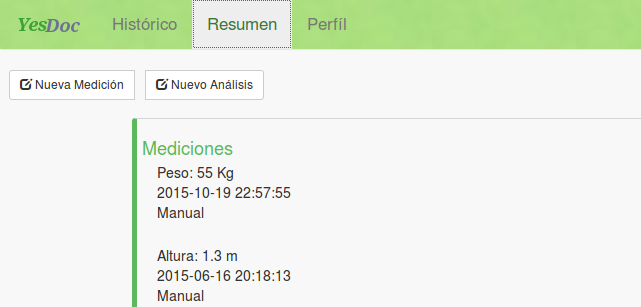
\includegraphics[width=0.5\textwidth]{img/5-boton_nuevo_analisis}
        \caption{vista para acceder a cargar nuevo análisis}
		\label{5-boton_nuevo_analisis}
    \end{figure}
    
    \begin{figure}[h]
        \centering
        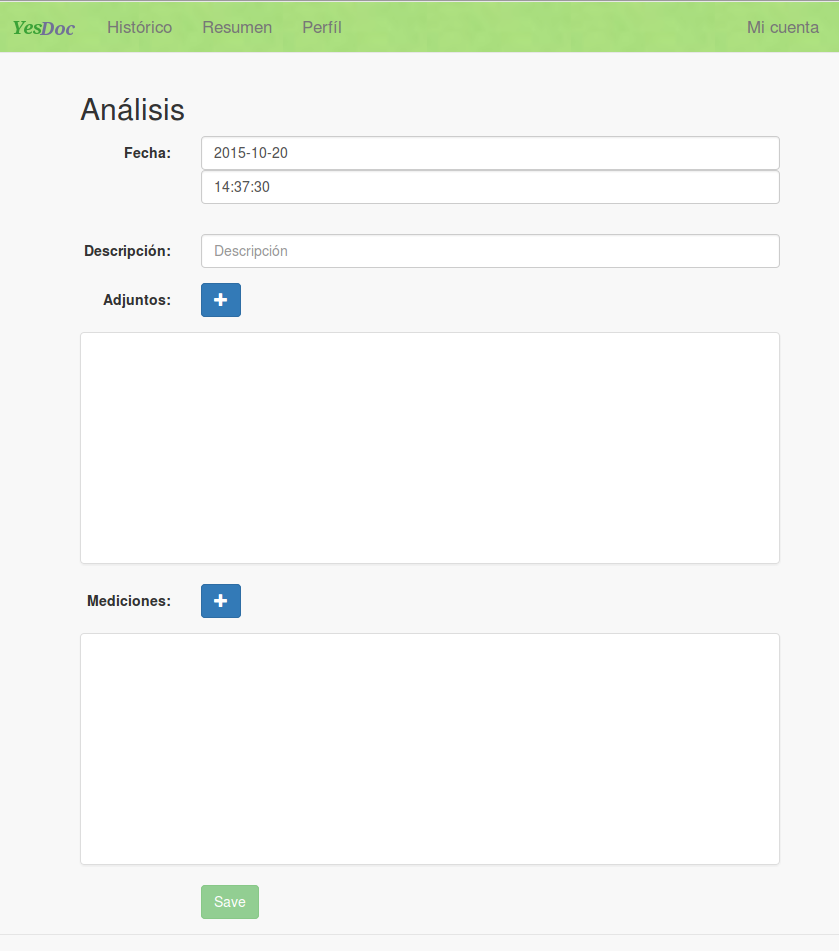
\includegraphics[width=0.5\textwidth]{img/5-crear_analisis}
        \caption{formulario para la creación de análisis}
		\label{5-crear_analisis}
    \end{figure}
    
    \begin{figure}[h]
        \centering
        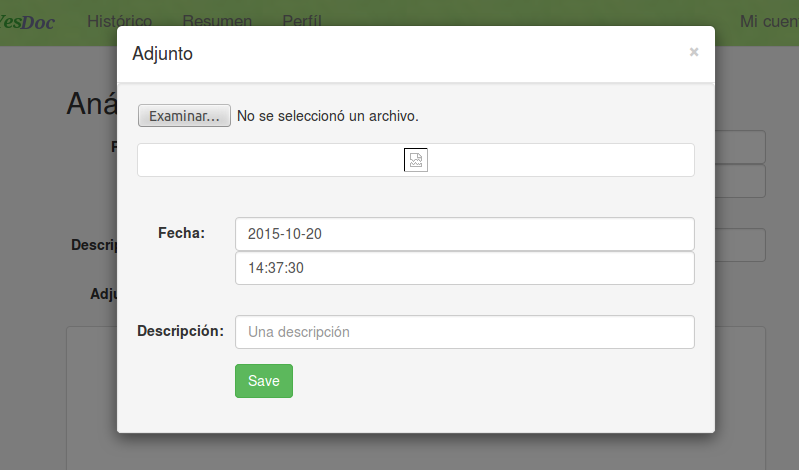
\includegraphics[width=0.5\textwidth]{img/5-cargar_img}
        \caption{formulario de carga de imágenes}
		\label{5-cargar_img}
    \end{figure}
    \begin{figure}[h]
        \centering
        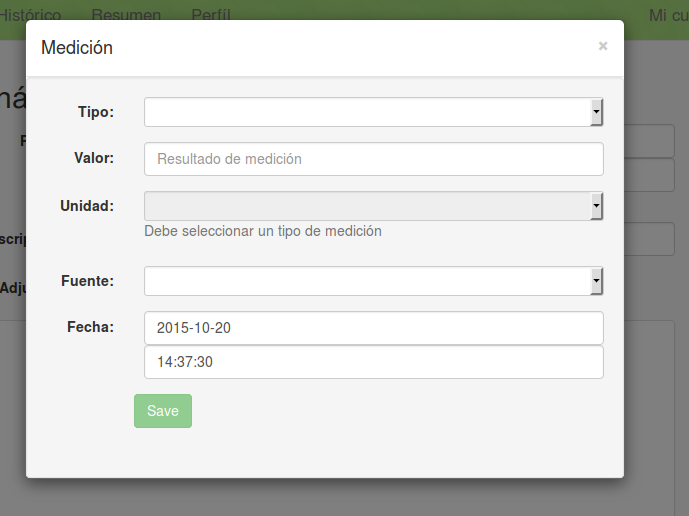
\includegraphics[width=0.5\textwidth]{img/5-cargar_medicion}
        \caption{formulario de carga de medición}
		\label{5-cargar_medicion}
    \end{figure}

    \begin{figure}[h]
        \centering
        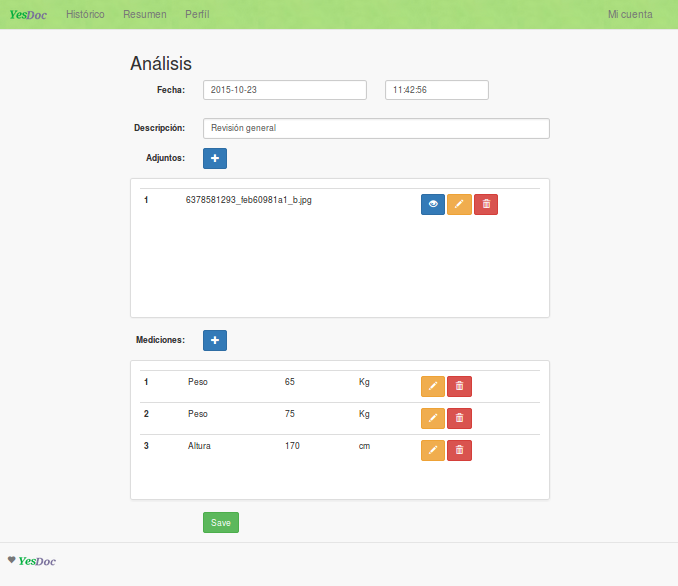
\includegraphics[width=0.5\textwidth]{img/5-mediciones_cargadas}
        \caption{Función de editar, borrar y visualizar}
		\label{5-mediciones_cargadas}
    \end{figure}


\clearpage

\subsection{Criterios de aceptación}

\begin{center}
\begin{longtable}{|p{0.5cm}|p{4cm}|p{4cm}|p{5cm}|}
\hline \hline \rowcolor[gray]{0.9}
	\multicolumn{4}{||c|}{\textbf{Criterio de aceptación}} \\
    \hline  \rowcolor[gray]{0.9}
        \textbf{Id} &
        \textbf{Contexto} &
        \textbf{Evento}&
        \textbf{Resultado} \\
    \hline
1&En caso de que exista una persona sin mediciones & cuando este desee observar sus mediciones  & El sistema no mostrará nada \\ \hline
 
2& Cuando el usuario registrado ingresa dos mediciones del mismo tipo  & y luego quiera consultarlas & El sistema solo le mostrará la ultima medición, del mismo tipo, realizada\\ \hline

3& Cuando el usuario seleccione una medición & y luego quiera editarla & El sistema le permitira la correspondiente edición\\ \hline

4& Si el usuario existe y no está logeado & y quiera ingresar a ver sus mediciones. & El sistema no le permitirá ingresar\\ \hline
  \end{longtable}
\end{center}


\subsection{Casos de prueba}

\subsubsection{Pruebas  de  integración  entre módulos del Sistema}












\begin{longtable}{|p{5cm}|p{5cm}|p{5cm}|}
\hline
Actor  & Sistema& Resultado Esperado \\ \hline

El usuario intenta ingresar al sistema & El sistema valida que el usuario con la contraseña ingresada exista & Se muestra un cartel de aviso de \textbf{usuario o contraseña invalido} \\ \hline

El usuario selecciona \textbf{nuevo perfil}, para
crear una cuenta en YesDoc 
& El sistema direcciona a la vista de creación de perfil
& Muestra formulario de creación de perfil.\\ \hline

 El usuario completa todos los campos y presiona save.
 Ingresa:
\begin{itemize}
	\item \textbf{Nombre de usuario:} Franco
	\item \textbf{Apellido:} Canizo
	\item \textbf{Fecha de nacimiento: }2015-10-90
	\item \textbf{Género: }Masculino
	\item \textbf{Email: }franco@franco
	\item \textbf{pass:}Franco

\end{itemize}
& El sistema anula el botón \textbf{guardar }hasta tanto el usuario cargue todos los campos. una vez cargado todos los campos,al presionar save, redirecciona al menu
de logueo de usuario.
& El sistema informa que ha sido generado su usuario y lo redireccion al formulario de login.
\\ \hline



El usuario ingresa 
	\textit{\begin{itemize}
		\item \textbf{Nombre de usuario:}Franco
		\item \textbf{Password: }Franco
	\end{itemize} }
&	El sistema valida usuario y contrasenña,genera el token, redirecciona a myProfileInformation y consulta a la API por la información personal \textbf{Figura \ref{5-login}}
& Se muestra la vista de perfil del usuario indicando sus datos personales
 \begin{itemize}
 		\item \textbf{Nombre de usuario:} Franco 
 		\item \textbf{Apellido: }Canizo 
 		\item \textbf{Fecha de nacimiento: }2015-10-90 
 		\item \textbf{Género: }Masculino
 	\end{itemize}

\\ \hline


Presiona el boton \textit{\textbf{``Editar Perfil'' }}
& El sistema carga la vista \textbf{``profileinformation-edit.html''}, carga la vista correspondiente , validaque el usuario se encuentre logueado pasándole el token que se encuentra almacenado en las cookies. Solicita ala API los datos del perfil y del genero
para rellenar el formulario.
& Se muestra el formulario con los datosdel perfil a editar.
\\ \hline



Cambia
\textit{
\begin{enumerate}
	\item \textbf{Nombre de usuario :} Franco Nicolás
\end{enumerate}}
&
& Muestra el cambio
\\ \hline


Guarda los datos presionando en \textit{\textbf{``guardar''}} 
& El sistema se conecta con la API yguarda los datos a través del método PUT. Redirecciona al perfil de usuario y muestra los datos cambiados
&
Se muestra el perfil con los.
\textit{
\begin{itemize}
	\item \textbf{Nombre de usuario:} Franco Ni-colas
	\item \textbf{Apellido:} CanizoFecha de
	\item \textbf{Nacimiento: }2015-10-90
	\item \textbf{Género:} Masculino
	\item \textbf{Email: }franco@franco
\end{itemize}
}
\\ \hline


El usuario presiona en \textbf{``Resumen'' } para ir a la sección donde se muestra una lista de cada medición con su último valor cargado.

& El sistema cambia la url por \textit{\textbf{``\#pro-fileMeasurements''}}, carga la vista correspondiente, valida que el usuario se encuentre logueado pasándole el token que se encuentra almacenado en las cookies y solicita al recurso de la API \textit{\textbf{``my/measurements/latest'' }}las últimas mediciones de cada tipo del usaurio. \textbf{Figura \ref{5-perfil}}

& Se muestra una pantalla con dos botones uno para la carga de medición
\textit{\textbf{``Nueva Medición'' }}y otro para la carga de análisis \textit{\textbf{``Nuevo Análisis''}}. No se muestra más datos porque es un usuario nuevo sin información.\textbf{Figura \ref{5-perfil_mediciones}}
\\ \hline



Selecciona en \textbf{``Nueva análisis'' }
& El sistema direcciona a la url \textit{\textbf{"analy-sis/new"}}, carga la vista correspondiente, valida que el usuario se encuentre logueado pasándole el token que se en-
cuentra almacenado en las cookies.

& Se muestra el formulario de carga de análisis \textbf{[Figura \ref{5-crear_analisis} ]}
\\ \hline



El usuario carga

\begin{itemize}
	\item \textbf{Fecha :}2015-09-30 16:10:59
	\item \textbf{Descripción: }revisión general
	\item Presionar en .\textbf{``Adjuntos''}

\end{itemize}

&
& El sistema muestra una ventana don-de se puede cargar las imágenes con la medición y fecha.\textbf{ [Figura  \ref{5-cargar_img}]}

\\ \hline



Selecciona una imagen "jpg.o "png", de-ja la fecha igual. 
&
& Se muestra una imagen previa de la imagen. Se muestra la fecha En descripción se muestra el nombre de la imagen
\\ \hline
 
 

Presiona \textbf{\textit{``guardar''}}
&
& Muestra
\begin{itemize}
	\item Nombre de la descripción de la imagen.
	\item Iconos de visualizar,
	\item \textbf{Iconos de editar}
	\item \textbf{Iconos de borrar.}
\end{itemize}
\\ \hline





Seleccionar \textit{\textbf{``cargar Medición'' }}
& El sistema se conecta con la API para solicitar tipo y fuentes de mediciones
& El sistema muestra una ventana donde  se puede cargar las mediciones con los siguientes datos:
\textbf{\begin{itemize}
	\item ``Tipo'',
\item ``Valor''
\item ``Unidad''
\item ``Fuente''
\item ``Fecha''
\end{itemize}}
\textbf{[Figura \ref{5-cargar_medicion}]}
\\ \hline




Selecciona tipo:\textit{\textbf{ "peso"} }
	& El sistema se conecta con la API para
solicitar unidades relacionadas al tipo de medición peso con \textbf{id:``1'' }. \textbf{[Figura \ref{5-crear_medicion}]}
& Muestra las posibles unidades correspondientes al tipo peso
\\ \hline



Ingresa
\begin{itemize}
	\item \textbf{Tipo:} ``Peso''
	\item \textbf{valor: }``65''
	\item \textbf{Unidad:} ``kilogramo''
	\item \textbf{Fuente: }``manual''
	\item \textbf{Fecha: }``2015:-09-30 16:10:59''
	\item \textbf{ Guardar}
\end{itemize}
&
& Mantiene la misma venta abierta y muestra un mensaje de aviso de que la
medición fue cargada con éxito.\textit{ \textbf{"Bien hecho se cargo una medición''}}
\\ \hline





Modificado el valor ingresado con anterioridad

\begin{itemize}
	\item \textbf{Tipo:} ``Peso''
	\item \textbf{valor: }``75''
	\item \textbf{Unidad:} ``kilogramo".
	\item \textbf{Fuente: }``manual"
	\item \textbf{Fecha: }2015:-10-10 16:10:59
	\item \textbf{ Guardar}
\end{itemize}
&
& Mantiene la misma venta abierta ymuestra un mensaje de aviso de que la
medicio'n fue cargada con éxito.\textbf{``Bien hecho se cargo una medición''}
\\ \hline




Selecciona



\begin{itemize}
	\item \textbf{Tipo:} ``altura'', modifica el va-lor ingresado con anterioridad
	por
	\item \textbf{valor: }``170''
	\item \textbf{Unidad:} ``centimetro".
	\item \textbf{Fuente: }``manual"
	\item \textbf{Fecha: }2015:-10-23 16:10:59
	\item \textbf{ Guardar}
\end{itemize}
&
&
Mantiene la misma venta abierta y muestra un mensaje de aviso de que
la medición fue cargada con éxito.\textit{\textbf{ ``Bien hecho se cargo una medición''}}
\\ \hline




Se selecciona el botón \textbf{"guardar"}
& El sistema consulta el perfil a la API para extraer el id el cual se usara para crear un análisis. Envia por POST a la API el análisis y realiza tres llamados mas a la API uno por cada medicióncargada.
Mantiene la misma venta abierta y muestra un mensaje de aviso de que
la medición fue cargada con éxito. Almacena en la API el path y el storage\_location de la imagen.Luego redirecciona la paágina a la url
\textit{\textbf{\#/profileMeasurements}}, valida que el token se encuentre activo, si no hay
errores solicta a la API las ultimas mediciones y muestra las mediciones

& En la vista de perfil de mediciones,Lista las -ltimas mediciones cargadas,
mostrando el peso cargado mas recien-temente

\begin{itemize}
	\item Peso: 65 Kg Fecha 2015-10-2314:42:56 Manual
	\item Altura: 170 cm 2015-10-2314:42:56 Manual

\end{itemize}


\\ \hline






Selecciona el icono de edición ubicado al lado de la medición \textit{Peso 65Kg}
& El sistema redirecciona \textbf{\#/measure-ments/103/edit}, verifica con la API que el token se encuentre activo, a partir del\textbf{ id} de la medición seleccionada para editar trae de la API el \textbf{tipo de medición, el valor, la unidad, la fuente y la fecha.}

& Se muestra un formulario con los datos de la medición precargadas
\begin{itemize}
	\item \textbf{Tipo:}Peso 
	\item \textbf{Valor: }65 
	\item \textbf{Unidad:} kilogramo
	\item \textbf{Fuente:}Manual 
	\item \textbf{Fecha:}2015-10-23 -14:42:56
\end{itemize}
\\ \hline





Cambia la \textit{\textbf{fecha y la hora} por 2015-5-13- 4:42:56 }y guarda los cambios.
& El sistema guarda la medición, redirecciona\textbf{ \#/profileMeasurements }valida el token, y solicita las últimas mediciones a la API

& Muestra la interfaz con las últimas mediciones 
\begin{itemize}
	\item Peso: 75 Kg 2015-10-23 14:42:56 Manual Altura: 170 cm 2015-10-23 14:42:56 Manual
\end{itemize}
\\ \hline





El usuario selecciona en \textit{\textbf{nueva medición}}
& El sistema redirecciona a \textbf{\#/measure-ments/new} valida contra la API que el Token se encuentra activo, luego traelos tipos de mediciones

& Muestra el formulario para cargar una medición con los siguientes valores 
\textbf{\begin{itemize}
	\item Tipo: 
	\item Valor:
	\item  Unidad: 
	\item Fuente: 
	\item Fecha:
\end{itemize}}
\\ \hline






El usuario selecciona en \textbf{``nueva medición''} 
\begin{itemize}
	\item \textbf{Tipo:}Peso
	\item \textbf{ Valor: }70
	\item\textbf{ Unidad:}-kilogramo
	\item \textbf{Fuente:}Manual
	\item \textbf{ Fecha:}2015-19-23 -14:42:56 
	\item \textbf{Guardar}
\end{itemize}

& El sistema redirecciona a \textbf{\#/profile-Measurementsvalida }contra la API que el Token se encuentra activo y luego trae las últimas mediciones

& Muestra la lista de últimas mediciones
\textbf{\begin{itemize}
	\item Peso: 75 Kg 2015-10-23 14:42:56 Manual
	\item Altura: 170 cm 2015-10-23 14:42:56 Ma-nual
\end{itemize}}
\\ \hline




Presionar en sección \textbf{``histórico''}
& El sistema redirecciona a\textbf{ \#/home }y se carga la vista correspondiente a  \textbf{  weight,} se verifica que el token este activo, setraen todas las medidas de tipo peso
& Se muestra una botonera con los tiposde mediciones , una gra'fica y una tabla con las 3 medidas de tipo \textbf{Peso}
\\ \hline




Presionar en sección \textbf{Peso }
& El sistema carga la vista correspondiente a height, se verifica que el token este activo, se traen todas las medidas de tipo peso
& Se muestra una botonera con los tipos de mediciones , una gráfica y una tabla con una medida \textbf{170 centímetros} de la altura.
\\ \hline





Presionar en sección \textit{\textbf{Análisis }} 
& El sistema carga la vista correspondiente a análisis, se verifica que el token este activo, se traen los análisis dela API
& Se muestra el análisis cargado con anterioridad mostrando la imagen, la descripción y la fecha seleccionada por el usuario.
\\ \hline






Selecciona el \textit{\textbf{Análisis}}
& El sistema carga la vista correspon-diente a \textbf{ \#/home/analyses}, se verifica que el token este activo, trae los datos y los archivos del análisis de la API
& Se muestran las imágenes (en este caso sólo una) y una tabla con las mediciones de ese análisis.
\\ \hline




Selecciona \textit{\textbf{Mi cuenta}}, luego \textit{\textbf{Cerrar Sesiónn}}
& El sistema direcciona \textbf{\#/logoof }y da debaja el token
& Se muestra la interface de login

\\ \hline


\end{longtable}







    \begin{figure}[h]
        \centering
        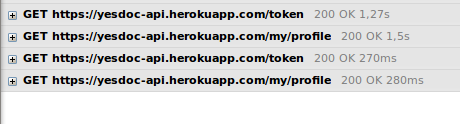
\includegraphics[width=0.5\textwidth]{img/5-login}
        \caption{Respuesta de la API al loguearse}
		\label{5-login}
    \end{figure}
    
        \begin{figure}[h]
        \centering
        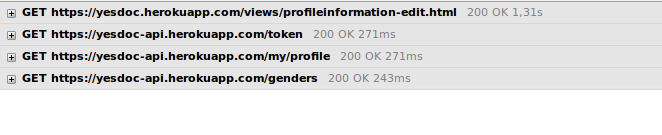
\includegraphics[width=0.5\textwidth]{img/5-perfil}
        \caption{Respuesta de la API al mostrar perfil}
		\label{5-perfil}
    \end{figure}
    
        \begin{figure}[h]
        \centering
        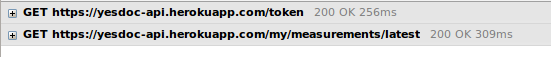
\includegraphics[width=0.5\textwidth]{img/5-resumen}
        \caption{Respuesta de la API al mostrar últimas mediciones}
		\label{5-resumen}
    \end{figure}
    
    \begin{figure}[h]
        \centering
        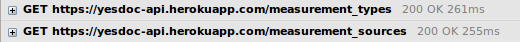
\includegraphics[width=0.5\textwidth]{img/5-crear_medicion}
        \caption{Respuesta de la API al crear nuevo análisis}
		\label{5-crear_medicion}
    \end{figure}
    
    
    
    
    \begin{figure}[h]
        \centering
        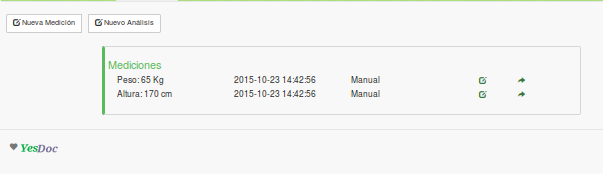
\includegraphics[width=0.5\textwidth]{img/5-perfil_mediciones}
        \caption{Perfil de mediciones}
		\label{5-perfil_mediciones}
    \end{figure}
    
    \begin{figure}[h]
        \centering
        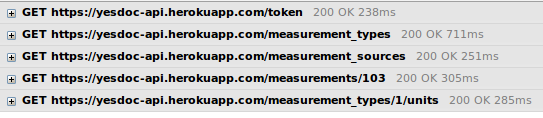
\includegraphics[width=0.5\textwidth]{img/5-editar_medicion}
        \caption{Respuesta de la API al editar mediciones}
		\label{5-editar_medicion}
    \end{figure}
    
    \begin{figure}[h]
        \centering
        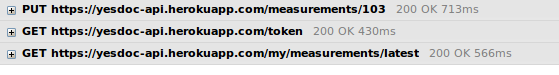
\includegraphics[width=0.5\textwidth]{img/5-fin_editar_medicion}
        \caption{Respuesta de la API al editar nuevo análisis}
		\label{5-fin_editar_medicion}
    \end{figure}
    
    \begin{figure}[h]
        \centering
        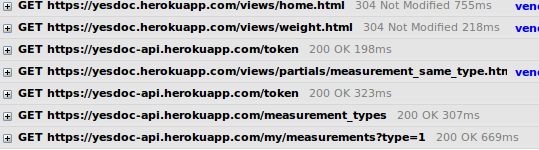
\includegraphics[width=0.5\textwidth]{img/5-mostrar_grafica}
        \caption{Respuesta de la API al mostrar gráficas}
		\label{5-mostrar_grafica}
    \end{figure}
    
    \begin{figure}[h]
        \centering
        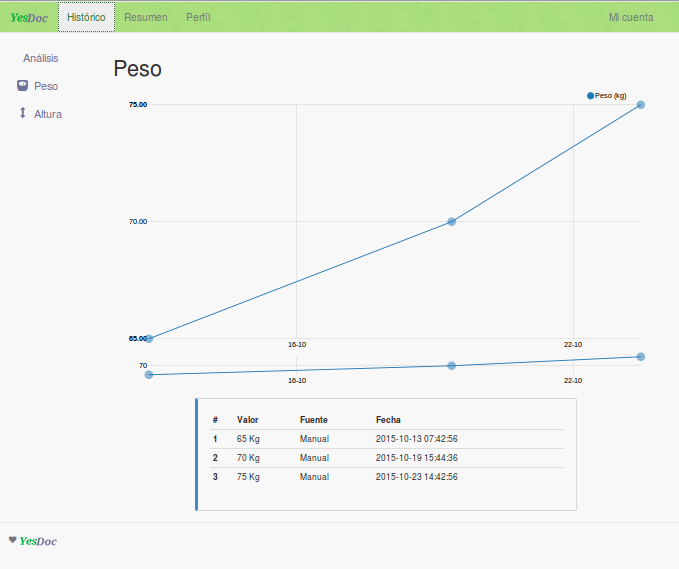
\includegraphics[width=0.5\textwidth]{img/5-grafica_medicion}
        \caption{Vista de gráfica y tablas de mediciones}
		\label{5-grafica_medicion}
    \end{figure}
    
    \begin{figure}[h]
        \centering
        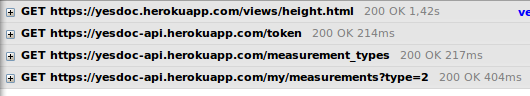
\includegraphics[width=0.5\textwidth]{img/5-grafica_altura}
        \caption{Respuesta de la API al mostrar la gráfica de altura}
		\label{5-grafica_altura}
    \end{figure}
    
    \begin{figure}[h]
        \centering
        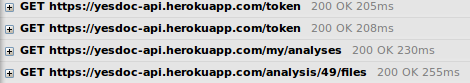
\includegraphics[width=0.5\textwidth]{img/5-mostrar_analisis}
        \caption{Respuesta de la API al mostrar los análisis}
		\label{5-mostrar_analisis}
    \end{figure}
    
    \begin{figure}[h]
        \centering
        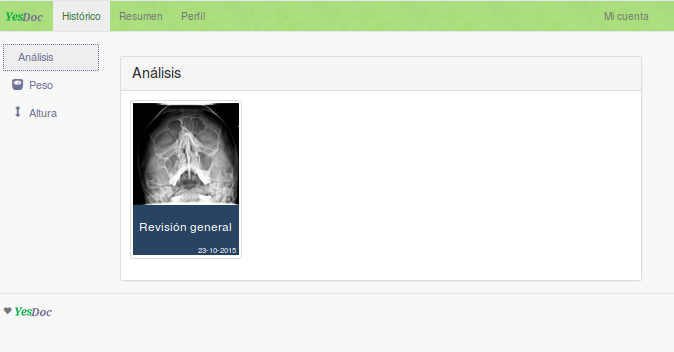
\includegraphics[width=0.5\textwidth]{img/5-mostrar_analisis_pag}
        \caption{Vista de la lista de análisis}
		\label{5-mostrar_analisis_pag}
    \end{figure}
    
    \begin{figure}[h]
        \centering
        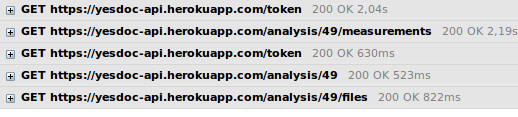
\includegraphics[width=0.5\textwidth]{img/5-analisis}
        \caption{Respuesta de la API al consultar los análisis}
		\label{5-analisis}
    \end{figure}
    
    \begin{figure}[h]
        \centering
        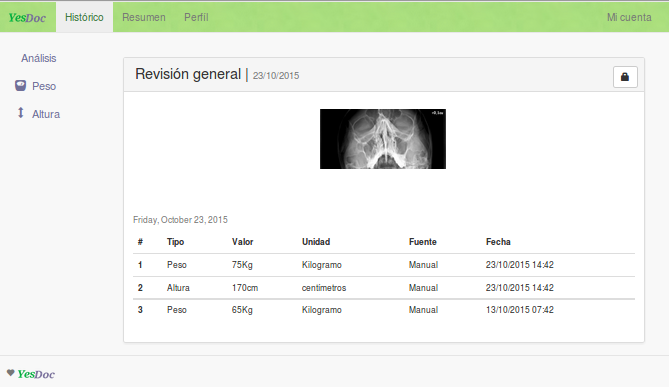
\includegraphics[width=0.5\textwidth]{img/5-contenido_analisis}
        \caption{Vista del contenido del análisis}
		\label{5-contenido_analisis}
    \end{figure}
    
    \begin{figure}[h]
        \centering
        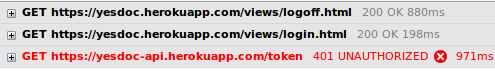
\includegraphics[width=0.5\textwidth]{img/5-logoff}
        \caption{Respuesta de la API al cerrar sesión}
		\label{5-logoff}
    \end{figure}
    



\clearpage



\subsubsection{ Pruebas de carga}

\subsubsection{ Pruebas de seguridad por niveles de usuarios}


\subsection{Pruebas ejecutadas}
Aqui se realizará una conclusión general de lo que se descubrió en las pruebas.
        %
	\begin{itemize}
		\item \textbf{¿Que fue bien?}
        	\begin{itemize}
				\item        Las cargas y ediciones se llevan a cabo correctamente.
			\end{itemize}

   		\item \textbf{¿Que se mejoró?}
        	\begin{itemize}
                \item \textbf{Cerrado} problema
			\end{itemize}

   		\item \textbf{¿Que se puede mejorar?}
        	\begin{itemize}
		        \item \textbf{Abierto} En el futuro se deberá mejorar ...
            \end{itemize}
        

	\end{itemize}
\clearpage


%%%%%%%%%%%%%%%%%%%%%%%%%%%%%%%%%%%%%%%%%%%%     FIN SPRINT 6   %%%%%%%%%%%%%%%%%%%%%%%%%%%%%%%%%%%%%%%%%%%%%%%%%%%%%%%5

\section{Sprint 7} % DROPBOX

\subsection{Planificación}

\textbf{Inicio: }Martes 11 de setiembre del 2015 

\textbf{Fin:} Martes 17 de octubre del 2015



\subsection{Descripción}

En este sprint se busca brindarle al usuario la funcionalidad para poder cargar imágenes, así este puede dejar un respaldo digital de lo que puede ser un análisis clínico o una imágen de radiografía y demás documentos médicos físicos. Para el mismo se plantean dos variantes, una local y otra en un servicio de almacenamiento, debido a que el desarrollo de ambas presentan sus diferencias y a su ves existen diferentes servicios de almacenamiento, se debe prever una estructura que soporte el impacto frente al cambio.

\subsection{User Stories relacionados}
La \textbf{Tabla \ref{US-Sprint6} } indicará las características de cada user story para guiarnos en el desarrollo del sprint.
% No entiendo porque para la tabla renderiza con ?? en el pdf.
\begin{table}[h]
    \label{US-Sprint6}
	%\resizebox{\textwidth}{!}{
    \centering
	\begin{tabular}{|l|p{9cm}|}
	\hline
        \multicolumn{1}{|c|}{\textbf{ID}} &
        \multicolumn{1}{|c|}{\textbf{Enunciado de la historia}} \\          
    \hline
        \textbf{US-1 } & Como paciente, quiero  añadir información de mi perfil de salud o mediciones regulares para que el médico cuente con más y mejor información al momento de realizar el diagnóstico. \\
     \hline 
    \hline
        \textbf{US-2 } & Como paciente, quiero añadir al sistema los estudios realizados para evitar posibles perdidas.\\
     \hline 
     \hline
        \textbf{US-16 } & Como paciente, quiero acceder a mis documentos desde cualquier lugar para hacer uso de ellos cuando los necesite.\\
     \hline   
     
    \end{tabular}
%     }
\end{table}

\subsection{Modelo de datos}
El Diagrama propio de este sprint se puede ver en la \textbf{Figura\ref{6-clases_file_upload}}, allí se indican exactamente las clases que se usarán en este sprint y que serán detalladas con detenimiento en el presente documento. Se recuerda que se ha realizado un Diagrama de clases específico para este sprint y puede variar en futuras iteraciones.
% Se fue a la mierda esta imágen
    \begin{figure}[h]
        \centering
        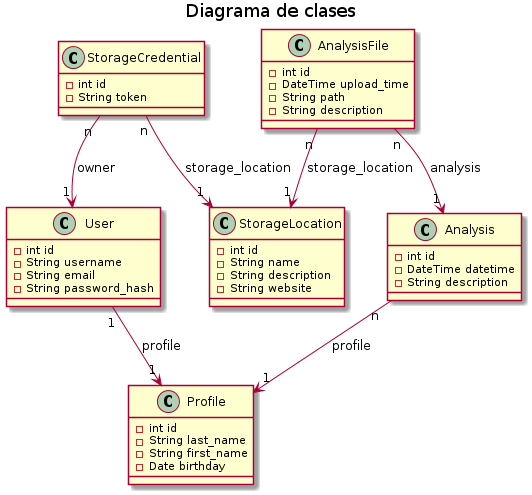
\includegraphics[width=0.5\textwidth]{img/dc_file_upload}
        \caption{Clases para la gestión de archivos.}
		\label{6-clases_file_upload}
    \end{figure}

\subsection{ Modelo funcional.} %Diagrama de clases
Se describirán las funciones usando como marco de apoyo el sprint Backlog, además se armará el diagrama de casos de uso del presente Sprint \textbf{[Figura \ref{6-cu_file_upload}]} que irá creciendo  medida se vaya avanzando en el proyecto.

    \begin{figure}[h]
        \centering
        \includegraphics[width=0.5\textwidth]{img/cu_file_upload}
        \caption{CU-Gestión de archivos}
		\label{6-cu_file_upload}
    \end{figure}


\textbf{EJEMPLO}
	{\scriptsize
	\begin{center} %sidewaystable
	\centering
	%\begin{adjustbox}{max width=\textheight}
    \resizebox{\textwidth}{!}{
	\begin{tabular}{|l|l|p{5cm}|l|}
	    \hline
	        \textbf{Area a cargo} &
	        \textbf{Responsable} &        
	        \textbf{Tarea} &
	        \textbf{US} \\
	    \hline
	    Back-end& Franco Canizo & Se define la estructura para la gestión de archivos & US-\ref{resumenInfo} \& US-\ref{infoSalud} \\ \hline
		\hline
	    Back-end& Franco Canizo & Se crea el adaptador para la gestión de archivos en dropbox y en los servidores de yesdoc, se crea el recurso para la carga de archivos de análisis. & US-\ref{resumenInfo} \& US-\ref{infoSalud} \\ \hline
        \hline
	    Back-end& Michael Manganiello & Se añaden las clases del dominio y funcionalidades para el manejo de análisis, archivos asociados, y la gestión de credenciales a diferentes servicios de almacenamiento personales del usuario & US-\ref{resumenInfo} \& US-\ref{infoSalud} \\ \hline
        \hline
	    Back-end& Michael Manganiello & Creación de la migración para los nuevos modelos & US-\ref{resumenInfo} \& US-\ref{infoSalud} \\ \hline
        \hline
	    Back-end& Michael Manganiello & Creación de fields y parsers para las representaciones de los nuevos recursos & US-\ref{resumenInfo} \& US-\ref{infoSalud} \\ \hline
        \hline
	    Back-end& Michael Manganiello & Correcciones generales de integración, claves de la aplicación en Dropbox, devolución y eliminación de archivos & US-\ref{resumenInfo} \& US-\ref{infoSalud} \\ \hline
	    \end{tabular}
        }
	    %\end{adjustbox}
    	\end{center}
	}
  
\subsubsection{Estructura conexión con diferentes medios de almacenamiento}
	Se define el paquete adapters en el cual se define una fábrica encargada de la creación del adaptador específico para la conexión y gestión de archivos con el medio de almacenamiento específico. Para la situación actual del sistema se definen dos adaptadores específicos, uno para el almacenamiento de archivos local en el servidor de YesDoc y otro para el almacentamiento de archivos en Dropbox. El \textbf{[Modelo \ref{6-dcd_file_upload}]} específico es el siguiente.

	\begin{figure}[h]
        \centering
        \includegraphics[width=0.9\textwidth]{img/dcd_file_upload}
        \caption{DCD-Carga de archivos}
		\label{6-dcd_file_upload}
    \end{figure}

\subsubsection{Creación de clases y funcionalidades para la gestión de archivos}

Se crean las clases del modelo lógico que definimos en la \textbf{Figura\ref{6-clases_file_upload}}, de cada una de estas se definen los atributos siguiendo la documentación de SQLAlchemy, ORM utilizado para mapeo de las entidades de la API, sus relaciones y funcionalidades. Un ejemplo es la clase StorageCredential:
\begin{lstlisting}[language=Python]

class StorageCredential(db.Model):
    # Attributes
    id          = db.Column(db.Integer, primary_key=True)
    token       = db.Column(db.String(255))
    # Foreign keys
    owner_id            = db.Column(db.Integer, db.ForeignKey('user.id'))
    storage_location_id = db.Column(db.Integer, db.ForeignKey('storage_location.id'))
    # Relationships
    owner            = db.relationship('User',
                                       backref=db.backref('storage_credentials', lazy='dynamic'))
    storage_location = db.relationship('StorageLocation',
                                       backref=db.backref('storage_credentials', lazy='dynamic'))

    def __init__(self, token, owner_id, storage_location_id):
        self.token               = token
        self.owner_id            = owner_id
        self.storage_location_id = storage_location_id

    def __repr__(self):
        return '<StorageCredential: %r>' % self.id
\end{lstlisting}

Esta clase del modelo guarda el token generado por el medio de almacenamiento, en este caso Dropbox, la relación con el StorageLocation que es el medio de almacenamiento y el User al que pertenece esta credencial.

\subsubsection{Creación de la migración para los nuevos modelos}

Una vez definidas las clases se ejecuta el comando db del script de python manager.py con la opción migrate lo que crea un script sql con la nueva versión de la base de datos. Luego se ejecuta con la opción upgrade lo que ejecuta el script y carga la base de datos. Eso es posible gracias al uso de las extensiones \textbf{flask-migrate} para las migraciones de la base de datos y \textbf{flask-script} para la ejecución de comandos externos.

\subsubsection{Creación de fields y parsers para las representaciones de los nuevos recursos}

Hemos definido nuevas clases. Para que el cliente se comunique con las mismas la API define recursos que manejan estas clases y representaciones para una interfaz única para con los recursos. El recurso que maneja las credenciales de almacenamiento es el siguiente:
\begin{lstlisting}[language=Python]
	class StorageCredentialList(Resource):
    @marshal_with(StorageCredentialFields.resource_fields, envelope='resource')
    def get(self):
        storage_credentials = StorageCredential.query.all()
        return storage_credentials
    @marshal_with(StorageCredentialFields.resource_fields, envelope='resource')
    def post(self):
        args = parser_post.parse_args()
        new_storage_credential = StorageCredential(args['token'],
                                                   args['owner_id'],
                                                   args['storage_location_id'])
        db.session.add(new_storage_credential)
        db.session.commit()
        return new_storage_credential, 201
\end{lstlisting}

La representación para las solicitudes HTTP del cliente al servidor.

\begin{lstlisting}[language=Python]
# Parser general
parser = reqparse.RequestParser()
parser.add_argument('token', type=str, required=True)
parser.add_argument('owner_id', type=is_valid_id, required=True)
parser.add_argument('storage_location_id', type=is_valid_id, required=True)
# Parser para recurso POST
parser_post = parser.copy()
# Parser para recurso PUT
parser_put = parser.copy()
# Parser para recurso POST con usuario autenticado
parser_post_auth = parser.copy().remove_argument('owner_id')
\end{lstlisting}

La representación para las respuestas del servidor al cliente.

\begin{lstlisting}[language=Python]
class StorageCredentialFields:
    resource_fields = {
        'id': fields.Integer,
        'token': fields.String,
        'owner': fields.Nested(UserFields.resource_fields),
        'storage_location': fields.Nested(StorageLocationFields.resource_fields),
    }
    required = ['id',
                'token',
                'owner',
                'storage_location']
\end{lstlisting}



\subsection {Salidas del Sistema - Incrementos}
\textbf{Carga de una credencial de almacenamiento}

Para la carga debemos utilizar el recurso que la API presenta con el identificador único URL \textbf{\/storage\_credentials}. Suponemos que previamente el usuario de prueba ha autorizado a nuestra aplicación a que utilice espacio del almacenamiento de su cuenta de dropbox y por lo tanto contamos con el token: ``Jl0\_uroqYBoAAAAAAAA
F6KUxPAlgAMTqFf9ES2S0zZl\_27V5QAmEn5V58IUxcck1''. Suponemos que ha sido cargado en API un usuario con id 1 y un storage location con id 2. Teniendo en cuenta la representación definida para la solicitud al recurso y que debemos usar el método POST para cargar la credencial, ejecutamos la siguiente linea CURL:

\begin{verbatim}
curl -i http://localhost:5000/storage_credentials -H "Content-Type: 
application/json" -X POST -d '{"token":"Jl0_uroqYBoAAAAAAAAF6KUxPAl
gAMTqFf9ES2S0zZl_27V5QAmEn5V58IUxcck1", "owner_id":"1", 
"storage_location_id":"1"}'
\end{verbatim}

La API nos responde con la siguiente respuesta:

\begin{lstlisting}[language=json]
HTTP/1.0 201 CREATED
Content-Type: application/json
Content-Length: 812
Server: Werkzeug/0.10.4 Python/2.7.6
Date: Tue, 20 Oct 2015 19:10:33 GMT

{
    "resource": {
        "id": 2, 
        "owner": {
            "email": "fncanizo@gmail.com", 
            "id": 1, 
            "profile": {
                "birthday": "1990-06-20", 
                "first_name": "Franco", 
                "gender": {
                    "description": "male gender", 
                    "id": 1, 
                    "name": "male"
                }, 
                "id": 1, 
                "last_name": "Canizo"
            }, 
            "username": "coco19"
        }, 
        "storage_location": {
            "description": "yesdoc file manager", 
            "id": 2, 
            "name": "YesDoc", 
            "website": "http://yesdoc.herokuapp.com"
        }, 
        "token": "Jl0_uroqYBoAAAAAAAAF6KUxPAlgAMTqFf9ES2S0zZl_27V5QAmEn5V58IUxcck1"
    }
}
\end{lstlisting}




\subsection{Criterios de aceptación}
\textbf{Ejemplo - esto se debe modificar}


\begin{center}
\begin{longtable}{|p{0.5cm}|p{4cm}|p{4cm}|p{5cm}|}
\hline \hline \rowcolor[gray]{0.9}
	\multicolumn{4}{||c|}{\textbf{Criterio de aceptación}} \\
    \hline  \rowcolor[gray]{0.9}
        \textbf{Id} &
        \textbf{Contexto} &
        \textbf{Evento}&
        \textbf{Resultado} \\
    \hline
1&En caso de que exista una persona sin mediciones & cuando este desee observar sus mediciones  & El sistema no mostrará nada \\ \hline
 

  \end{longtable}
\end{center}


\subsection{Casos de prueba}

\subsubsection{Pruebas  de  integración  entre módulos del Sistema}

\subsubsection{ Pruebas de carga}

\subsubsection{ Pruebas de seguridad por niveles de usuarios}


\subsection{Pruebas ejecutadas}
Aqui se realizará una conclusión general de lo que se descubrió en las pruebas.
        %
	\begin{itemize}
		\item \textbf{¿Que fue bien?}
        	\begin{itemize}
				\item        Las cargas y ediciones se llevan a cabo correctamente.
			\end{itemize}

   		\item \textbf{¿Que se mejoró?}
        	\begin{itemize}
                \item \textbf{Cerrado} problema
			\end{itemize}

   		\item \textbf{¿Que se puede mejorar?}
        	\begin{itemize}
		        \item \textbf{Abierto} En el futuro se deberá mejorar ...
            \end{itemize}
        

	\end{itemize}

%%%%%%%%%%%%%%%%%%%%%%%%%%%%    SPRINT 6   %%%%%%%%%%%%%%%%%%%%%%%%
\section{Sprint 8} % COMENTARIO

\subsection{Planificación}

\textbf{Inicio: }?? del 2015 

\textbf{Fin:} ?? de octubre del 2015



\subsection{Descripción}

\subsection{User Stories relacionados}
La \textbf{Tabla \ref{US-Sprint3} } indicará las características de cada user story para guiarnos en el desarrollo del sprint.
%\textbf{ESTO ES UN EJEMPLOOOO HAY QUE INDICAR TDOS LOS US RELACIONADO}
\begin{table}[h]
    \label{US-Sprint3}
	%\resizebox{\textwidth}{!}{
    \centering
	\begin{tabular}{|l|p{9cm}|}
	\hline
        \multicolumn{1}{|c|}{\textbf{ID}} &
        \multicolumn{1}{|c|}{\textbf{Enunciado de la historia}} \\          
    \hline
        \textbf{US-2 } & Como paciente, quiero añadir al sistema los estudios realizados para evitar posibles perdidas.\\
     \hline 
     
    \end{tabular}
%     }
\end{table}

\subsection{Modelo de datos}
El Diagrama propio de este sprint se puede ver en la \textbf{Figura\ref{2-modelo_datos_general}}, allí se indican exactamente las clases que se usarán en este sprint y que serán detalladas con detenimiento en el presente documento. Se recuerda que se ha realizado un Diagrama de clases tentativo que se puede ver en la \textbf{Figura \ref{2-modelo_datos_general}}, dicho diagrama  será utilizado como base para este sprint y posee un alcance limitado el cual se irá modificando a medida que se profundice en los temas.


%\textbf{AÑADIR DIAGRAMA DE CLASEEES}


\subsection{ Modelo funcional.} %Diagrama de clases
Se describirán las funciones usando como marco de apoyo el sprint Backlog, además se armará el diagrama de casos de uso del presente Sprint \textbf{[Figura \ref{2-caso_de_uso}]} que irá creciendo  medida se vaya avanzando en el proyecto.


%\textbf{CARGAR CASO DE USOO}
    \begin{figure}[h]
        \centering
        \includegraphics[width=0.5\textwidth]{img/2-caso_de_uso}
        \caption{formulario de edición de perfil}
		\label{2-caso_de_uso}
    \end{figure}


%\textbf{EJEMPLO}
	{\scriptsize
	\begin{center} %sidewaystable
	\centering
	%\begin{adjustbox}{max width=\textheight}
    \resizebox{\textwidth}{!}{
	\begin{tabular}{|l|l|l|l|}
	    \hline
	        \textbf{Area a cargo} &
	        \textbf{Responsable} &        
	        \textbf{Tarea} &
	        \textbf{US} \\
	    \hline
	    Front-end& Ivan Terreno & Generación de controladores para consumir Json de la Api relacionados a la API  & US-\ref{resumenInfo} \& US-\ref{infoSalud} \\ \hline

	    \end{tabular}
        }
	    %\end{adjustbox}
    	\end{center}
	}
  
 
  
    %\textbf{Describimos cada tarea???}
\subsubsection{Tarea a describir}


\subsection {Salidas del Sistema - Incrementos}
\textbf{Esto es un ejemplo. Debe listarse las pantallas y explicar que hacen}
\begin{enumerate}
    \item \textbf{Presentación de las últimas mediciones}  \textbf{[Figura  \ref{perfil_medicion}]} con posibilidad de edición de cada una de las mediciones. Los datos posible  a presentar son altura, peso, grasa corporal y glucosa. 
    
    La interfaz mostrará el valor de la medición, la fecha y hora en que fue realizada y la fuente que se utilizó para dicha medición.

\end{enumerate}

    




\subsection{Criterios de aceptación}
\textbf{Ejemplo - esto se debe modificar}


\begin{center}
\begin{longtable}{|p{0.5cm}|p{4cm}|p{4cm}|p{5cm}|}
\hline \hline \rowcolor[gray]{0.9}
	\multicolumn{4}{||c|}{\textbf{Criterio de aceptación}} \\
    \hline  \rowcolor[gray]{0.9}
        \textbf{Id} &
        \textbf{Contexto} &
        \textbf{Evento}&
        \textbf{Resultado} \\
    \hline
1&En caso de que exista una persona sin mediciones & cuando este desee observar sus mediciones  & El sistema no mostrará nada \\ \hline
 

  \end{longtable}
\end{center}


\subsection{Casos de prueba}

\subsubsection{Pruebas  de  integración  entre módulos del Sistema}

\subsubsection{ Pruebas de carga}

\subsubsection{ Pruebas de seguridad por niveles de usuarios}


\subsection{Pruebas ejecutadas}
Aqui se realizará una conclusión general de lo que se descubrió en las pruebas.
        %
	\begin{itemize}
		\item \textbf{¿Que fue bien?}
        	\begin{itemize}
				\item        Las cargas y ediciones se llevan a cabo correctamente.
			\end{itemize}

   		\item \textbf{¿Que se mejoró?}
        	\begin{itemize}
                \item \textbf{Cerrado} problema
			\end{itemize}

   		\item \textbf{¿Que se puede mejorar?}
        	\begin{itemize}
		        \item \textbf{Abierto} En el futuro se deberá mejorar ...
            \end{itemize}
        

	\end{itemize}

%%%%%%%%%%%%%%%%%%%%%%%%%%%%    SPRINT 7   %%%%%%%%%%%%%%%%%%%%%%%%

\section{Sprint 8} % COMPARTICIÓN

\subsection{Planificación}

\textbf{Inicio: }?? del 2015 

\textbf{Fin:} ?? de octubre del 2015



\subsection{Descripción}

\subsection{User Stories relacionados}
La \textbf{Tabla \ref{US-Sprint3} } indicará las características de cada user story para guiarnos en el desarrollo del sprint.
\textbf{ESTO ES UN EJEMPLOOOO HAY QUE INDICAR TDOS LOS US RELACIONADO}
\begin{table}[h]
    \label{US-Sprint3}
	%\resizebox{\textwidth}{!}{
    \centering
	\begin{tabular}{|l|p{9cm}|}
	\hline
        \multicolumn{1}{|c|}{\textbf{ID}} &
        \multicolumn{1}{|c|}{\textbf{Enunciado de la historia}} \\          
    \hline
        \textbf{US-2 } & Como paciente, quiero añadir al sistema los estudios realizados para evitar posibles perdidas.\\
     \hline 
     
    \end{tabular}
%     }

\end{table}

\subsection{Modelo de datos}
El Diagrama propio de este sprint se puede ver en la \textbf{Figura\ref{2-modelo_datos_general}}, allí se indican exactamente las clases que se usarán en este sprint y que serán detalladas con detenimiento en el presente documento. Se recuerda que se ha realizado un Diagrama de clases tentativo que se puede ver en la \textbf{Figura \ref{2-modelo_datos_general}}, dicho diagrama  será utilizado como base para este sprint y posee un alcance limitado el cual se irá modificando a medida que se profundice en los temas.


\textbf{AÑADIR DIAGRAMA DE CALSEEES}


\subsection{ Modelo funcional.} %Diagrama de clases
Se describirán las funciones usando como marco de apoyo el sprint Backlog, además se armará el diagrama de casos de uso del presente Sprint \textbf{[Figura \ref{2-caso_de_uso}]} que irá creciendo  medida se vaya avanzando en el proyecto.


\textbf{CARGAR CASO DE USOO}
    \begin{figure}[h]
        \centering
        \includegraphics[width=0.5\textwidth]{img/2-caso_de_uso}
        \caption{formulario de edición de perfil}
		\label{2-caso_de_uso}
    \end{figure}


\textbf{EJEMPLO}
	{\scriptsize
	\begin{center} %sidewaystable
	\centering
	%\begin{adjustbox}{max width=\textheight}
    \resizebox{\textwidth}{!}{
	\begin{tabular}{|l|l|l|l|}
	    \hline
	        \textbf{Area a cargo} &
	        \textbf{Responsable} &        
	        \textbf{Tarea} &
	        \textbf{US} \\
	    \hline
	    Front-end& Ivan Terreno & Generación de controladores para consumir Json de la Api relacionados a la API  & US-\ref{resumenInfo} \& US-\ref{infoSalud} \\ \hline

	    \end{tabular}
        }
	    %\end{adjustbox}
    	\end{center}
	}
    
    \textbf{Describimos cada tarea???}
\subsubsection{Creación de página de mediciones}

\subsection {Salidas del Sistema - Incrementos}
\textbf{Esto es un ejemplo. Debe listarse las pantallas y explicar que hacen}
\begin{enumerate}
    \item \textbf{Presentación de las últimas mediciones}  \textbf{[Figura  \ref{perfil_medicion}]} con posibilidad de edición de cada una de las mediciones. Los datos posible  a presentar son altura, peso, grasa corporal y glucosa. 
    
    La interfaz mostrará el valor de la medición, la fecha y hora en que fue realizada y la fuente que se utilizó para dicha medición.

\end{enumerate}

    




\subsection{Criterios de aceptación}
\textbf{Ejemplo - esto se debe modificar}
\begin{center}
\begin{longtable}{|p{0.5cm}|p{4cm}|p{4cm}|p{5cm}|}
\hline \hline \rowcolor[gray]{0.9}
	\multicolumn{4}{||c|}{\textbf{Criterio de aceptación}} \\
    \hline  \rowcolor[gray]{0.9}
        \textbf{Id} &
        \textbf{Contexto} &
        \textbf{Evento}&
        \textbf{Resultado} \\
    \hline
1&En caso de que exista una persona sin mediciones & cuando este desee observar sus mediciones  & El sistema no mostrará nada \\ \hline
 

  \end{longtable}
\end{center}


\subsection{Casos de prueba}

\subsubsection{Pruebas  de  integración  entre módulos del Sistema}

\subsubsection{ Pruebas de carga}

\subsubsection{ Pruebas de seguridad por niveles de usuarios}


\subsection{Pruebas ejecutadas}
Aqui se realizará una conclusión general de lo que se descubrió en las pruebas.
        %
	\begin{itemize}
		\item \textbf{¿Que fue bien?}
        	\begin{itemize}
				\item        Las cargas y ediciones se llevan a cabo correctamente.
			\end{itemize}

   		\item \textbf{¿Que se mejoró?}
        	\begin{itemize}
                \item \textbf{Cerrado} problema
			\end{itemize}

   		\item \textbf{¿Que se puede mejorar?}
        	\begin{itemize}
		        \item \textbf{Abierto} En el futuro se deberá mejorar ...
            \end{itemize}
        

	\end{itemize}











%Desarrollo e implementación
\section{Programación y documentación}
Este apartado tiene como objetivo describir en que consiste el desarrollo y documentación asociado a una parte del sistema a mostrar, para ejemplificar a partir de las historias de usuario involucradas, cómo es la forma de trabajo.
	

Se ha seleccionado dos \textit{EPICS} del sistema, que a continuación se detalla, para describirlos, el código desarrollado se encuentra en el \textbf{Anexo \ref{codigo}}
\begin{enumerate}
\item \textit{\textbf{Permitir al usuario añadir los análisis realizados }}
%(Perfil de mediciones con carga sencilla de mediciones Carga de mediciones completa incluyendo a los analisis.

\textbf{User Stories relacionados}
    \begin{itemize}
        \item \textbf{US-2 }Como paciente, quiero añadir al sistema los estudios realizados para evitar posibles perdidas.
        \item \textbf{US-5 }Como paciente quiero que los sistemas de salud existentes puedan cargar sus resultados directamente en mi carpeta de salud para centralizar mi información
        \item  \textbf{US-7} Como paciente quiero categorizar mis estudios por rama de medicina, para lograr una mejor organización y navegabilidad en el sistema
        \item \textbf{US-8} Como laboratorio, quiero cargar información de un paciente en su cuenta para ahorrarle las molestias de volver
    \end{itemize}
\item \textbf{\textit{Permitir a los usuarios generar vistas de su información a lo largo del tiempo, a través de gráficas , tablas y resúmenes }}
%(Histórico de mediciones que permite ver el avance de las mediciones).

\textbf{User Stories relacionados}
    \begin{itemize}
        \item \textbf{US-17} Como paciente quiero ver gráficas que resuman mi información en particular para poder ver mis cambios a lo largo de la historia.
        \item \textbf{US-15} Como médico quiero ver gráficas que resuman la información de un paciente para poder ver sus cambios a lo largo de la historia y así apoyar la toma de decisiones y el diagnóstico.
    \end{itemize}
\end{enumerate}
Estos User Stories fueron desarrollados en los Sprints anteriores...

\subsection{Descripción de la funcionalidad} % ya se dijo en el sprint
\subsubsection{Cargar análisis}
\subsubsection{Generación de tablas y gráficas de mediciones}

\subsection{Diseño Técnico}
En este documento se efectúa un diseño ñógico que permite, a partir de la arquitectura y la descripción del requisito en la fase de análisis, dar soporte a la implementación de la funcionalidad.

Aquí se describen los artificios utilizados a nivel técnico para resolver el problema que se planteó en la historia de usuario. Se incluyen diagrmas de clases, modelos de datos, etc. Para esto se utiliza un documento compuesto de 4 partes
\begin{itemize}
\item Objetivo

El objetivo consiste en poder cargar mediciones de distintos tipos, de diferentes fuente y en diferentes unidades para un usuario con un perfil creado.

\item Diseño de a fase de datos

Se requiere la preparación de datos para popular las tablas que guardan los datos de los objetos de las siguientes \textbf{[clases \ref{2-caso_de_uso}]}.

    \begin{figure}[h]
        \centering
        \includegraphics[width=0.5\textwidth]{img/dc_mediciones}
        \caption{DC-Mediciones}
		\label{2-caso_de_uso}
    \end{figure}

\item Diseño API REST

%------------------------ API REST --------------------------------

La estructura de nuestra api busca aplicar lo más fielmente posible el principio arquitectónico que define  REST, Representational State Transfer, el cual consiste en un estilo de arquitectura de software para construir web services escalables. La comunicación con la api es a través del protocolo HTTP y se busca utilizar los mismos verbos, GET, POST, PUT, entre otros. Para que la API sea REST cumple con las siguientes 6 restricciones según establece el paper que introduce REST:
\begin{enumerate}
	\item Cliente-Servidor
    
    La API debe estar separada del cliente y se comunican a través del protocolo de red HTTP.
    
    \item Stateless
    
    No se mantienen sesiones, cada solicitud y respuesta están totalmente aisladas unas de otras. Los clientes deben ser autenticados en cada solicitud. Un gris en stateless podría ser usar cookies para almacenar información que se mantiene entre solicitudes.
    
    \item Cache
    
    El servidor debe proveer directivas de cacheo que indiquen a intermediarios las condiciones bajo las cuales cachear información.
    
    \item Uniform interface
    
    \textbf{Identificación de recursos}, los recursos son todas las entidades en el dominio de nuestra aplicación. Cada recurso tiene un único identificador (URL), accediendo a los identificadores podemos obtener colecciones de representación de recursos.
    
    \textbf{Representación de recursos}, el cliente se comunica y opera con los recursos a través de las representaciones que la api ofrece. Las representaciones pueden presentarse en distintos formatos (en nuestro caso JSON). Las representaciones se separan de los recursos.
    
    \textbf{Mensajes descriptivos}, tanto solicitudes como respuestas cliente-servidor están aisladas completamente por lo que no hay información relacionada entre sucesivas solicitudes y respuestas.
    
    \textbf{Hypermedia}, plantea una forma de usar la api a través de enlaces, el cliente descubre nuevos recursos a través de la información que brindan los recursos previamente descubiertos.
    
    \item Layered system
    Cliente y servidor no necesariamente se comunican directamente, pueden existir intermediarios.
    
    \item Code on demand
    Restricción opcional, el servidor provee código que el cliente puede utilizar.
    
\end{enumerate}

La estructura de nuestra API se presenta de la siguiente forma:

\begin{comment}
		imágen directorios
\end{comment}

Uno de los archivos principales es el archivo de configuración, Flask no necesita mucha configuración, solo una serie de pares clave-valor. En nuestra aplicación tenemos 4 modos en los que puede correr la aplicación. development, staging, testing and production.
	Lo que hacemos es definir una clase principal Config donde colocamos las variables de configuración que aplicarán a todas las configuraciones, y luego tres subclases enlas cuales determinamos configuraciones que son específicas para cada uno de los tipos de configuración. La clave Secret key la usamos para encriptación de todas las fuentes. Tanto flask como las extensiones usan secret key para encriptar.
	Para definir el modo de configuración el valor lo tomamos de una variable del environment y como mostramos en el código, la configuración por defecto es la de producción.
    
\begin{lstlisting}[language=Python]
class Config(object):
    DEBUG = False
    TESTING = False
    CSRF_ENABLED = True
    # encriptacion de todas las fuentes
    SECRET_KEY = 'this-really-needs-to-be-changed'
    SQLALCHEMY_DATABASE_URI = os.environ.get('DATABASE_URL', 'postgresql:///salud_dev?client_encoding=utf8')
    Parametro que indica si el parser de argumentos debe devolver la totalidad de los errores encontrados en una
    peticion a la API (True), o solo el primer error (False).
    BUNDLE_ERRORS = True
    # Directorio donde guardaremos el archivo
    #UPLOAD_FOLDER = '/tmp'
    #ALLOWED_IMG_EXTENSIONS = set(['png'])
    UPLOADED_PHOTOS_DEST = '/tmp/imagenes'
    MAX_CONT_IMG_LENGTH = 6 * 1024 * 1024
    uploaded_photos = UploadSet('photos', IMAGES)
    # Claves, publica y privada, de autenticacion de la aplicacion en Dropbox.
    DROPBOX_APP_KEY = 'i7u47ht1t730nar'
    DROPBOX_APP_SECRET = os.environ.get('DROPBOX_APP_SECRET', '')

class ProductionConfig(Config):
    DEBUG = False

class StagingConfig(Config):
    DEVELOPMENT = True
    DEBUG = True
    
class DevelopmentConfig(Config):
    DEVELOPMENT = True
    DEBUG = True
    
class TestingConfig(Config):
    TESTING = True
\end{lstlisting}

Otro de los archivos importantes es el que presenat el código de inicio de la aplicación, en este encontramos tres puntos principales, en primer lugar la creación de la instancia de flask para nuestra api

\begin{lstlisting}[language=Python]
app = Flask(__name__)
flask_config_mode = os.getenv('FLASK_CONFIG_MODE', 'production')
app.config.from_object(get_config_class(flask_config_mode))
\end{lstlisting}

El punto donde definimos los identificadores para acceder a un determinado recurso, usando el método add\_resource de la extensión de flask, \textbf{flaskRESTful} que nos permite registrar una ruta en flask. Esto permite que nuestra API presente una interfaz única.

\begin{lstlisting}
api.add_resource(GenderView, '/genders/<int:id>')
api.add_resource(GenderList, '/genders')
api.add_resource(ProfileView, '/profiles/<int:id>')
api.add_resource(ProfileList, '/profiles')
api.add_resource(MeasurementView, '/measurements/<int:id>')
api.add_resource(MeasurementList, '/measurements')
api.add_resource(MeasurementSourceView, '/measurement_sources/<int:id>')
api.add_resource(MeasurementSourceList, '/measurement_sources')
api.add_resource(MeasurementTypeView, '/measurement_types/<int:id>')
api.add_resource(MeasurementTypeList, '/measurement_types')
api.add_resource(MeasurementUnitView, '/measurement_units/<int:id>')
api.add_resource(MeasurementUnitList, '/measurement_units')
api.add_resource(PermissionTypeList, '/permission_types')
\end{lstlisting}

Cabe destacar que las rutas expuestan presentan un resumen y no la totalidad de rutas que presenta acutalmente la API.
Como podemos observar, el cliente tendrá acceso a la representación de respuesta del recurso MeasurementList solo enviando una representación correcta en una solicitud a la url http://dominio\_raiz/measurements.

Por último, el tercer punto, se ubica en otro archivo y nos permite iniciar la API.

\begin{lstlisting}[language=Python]
#!flask/bin/python

# -*- coding: utf-8 -*-

from app import app

if __name__ == '__main__':
    app.run(host='0.0.0.0')
\end{lstlisting}

Ejecutando este script de python iniciamos la API.
Los recursos de la API presentan la siguiente estructura:

\begin{lstlisting}[language=Python]
class MeasurementList(Resource):
    @marshal_with(MeasurementFields.resource_fields, envelope='resource')
    def get(self):
        measurements = Measurement.query.all()
        return measurements
    @marshal_with(MeasurementFields.resource_fields, envelope='resource')
    def post(self):
        args = parser_post.parse_args()
        new_measurement = Measurement(args['datetime'],
                                      args['value'],
                                      args['analysis_id'],
                                      args['profile_id'],
                                      args['measurement_source_id'],
                                      args['measurement_type_id'],
                                      args['measurement_unit_id'])
        db.session.add(new_measurement)
        db.session.commit()
        return new_measurement, 201
\end{lstlisting}
Como vemos el recurso define dos métodos, uno con el nombre get y otro con el nombre post, estos métodos responden a las solicitudes HTTP al identificador /measurements, que indiquen en el atributo method el operador GET y POST respectivamente. En el caso del recurso indicado, la solicitud con operando GET devolverá al cliente una colección de representaciones de medidas en la base de datos mientras que con el operando POST cargará una nueva medida. La clase del modelo que para las medidas se encuentra en el paquete models del paquete mod\_profiles

\begin{lstlisting}[language=Python]
class Measurement(db.Model):
    # Attributos, columnas de la base de datos
    id       = db.Column(db.Integer, primary_key=True)
    datetime = db.Column(db.DateTime)
    value    = db.Column(db.Float)
    # Claves foraneas
    analysis_id           = db.Column(db.Integer, db.ForeignKey('analysis.id'))
    profile_id            = db.Column(db.Integer, db.ForeignKey('profile.id'))
    measurement_source_id = db.Column(db.Integer, db.ForeignKey('measurement_source.id'))
    measurement_type_id   = db.Column(db.Integer, db.ForeignKey('measurement_type.id'))
    measurement_unit_id   = db.Column(db.Integer, db.ForeignKey('measurement_unit.id'))
    # Relaciones entre tablas
    analysis           = db.relationship('Analysis',
                                         backref=db.backref('measurements', lazy='dynamic'))
    profile            = db.relationship('Profile',
                                         backref=db.backref('measurements', lazy='dynamic'))
    measurement_source = db.relationship('MeasurementSource',
                                         backref=db.backref('measurements', lazy='dynamic'))
    measurement_type   = db.relationship('MeasurementType',
                                         backref=db.backref('measurements', lazy='dynamic'))
    measurement_unit   = db.relationship('MeasurementUnit',
                                         backref=db.backref('measurements', lazy='dynamic'))
    # Constructor de la clase
    def __init__(self, datetime, value, analysis_id, profile_id, source_id, type_id, unit_id):
        self.datetime              = datetime
        self.value                 = value
        self.analysis_id           = analysis_id
        self.profile_id            = profile_id
        self.measurement_source_id = source_id
        self.measurement_type_id   = type_id
        self.measurement_unit_id   = unit_id
    # Representacion string de la instancia
    def __repr__(self):
        return '<Measurement: %r>' % (self.datetime)
\end{lstlisting}

La definición de la clase del modelo se hace de acuerdo a lo que establece el ORM usado por el equipo, \textbf{SQLAlchemy}.

El nombre de la tabla en la base de datos se genera automáticamente cambiando CamelCase por camel\_case, el atributo column define la columna de la base de datos y las restricciones que se aplican a la misma, el atributo relationship define la relación entre las distintas tablas.

Como establecimos en la introducción de REST, la API funciona recibiendo solicitudes HTTP y respondiendo a las mismas. La API define identificadores a los cuales los clientes pueden referir, para que las solicitudes sean aceptadas. Éstas deben enviar información en el cuerpo que esté de acuerdo a las representaciones que definimos para la API, en nuestro caso, las representaciones deben ser del tipo JSON y tener los pares clave-valor que define el parser del recurso en el paquete parsers en common. Para el caso actual de medidas se define el siguiente parser.

\begin{lstlisting}[language=Python]
# Parser general
parser = reqparse.RequestParser()
parser.add_argument('datetime', type=is_valid_previous_datetime, required=True)
parser.add_argument('value', type=float, required=True)
parser.add_argument('analysis_id', type=is_valid_id, required=True)
parser.add_argument('profile_id', type=is_valid_id, required=True)
parser.add_argument('measurement_source_id', type=is_valid_id)
parser.add_argument('measurement_type_id', type=is_valid_id, required=True)
parser.add_argument('measurement_unit_id', type=is_valid_id, required=True)

# Parser para recurso POST
parser_post = parser.copy()

# Parser para recurso PUT
parser_put = parser.copy()

# Parser para recurso POST con usuario autenticado
parser_post_auth = parser.copy().remove_argument('profile_id')
\end{lstlisting}

Como podemos ver en la tercer línea, la API recibe un dato con el nombre ‘datetime’, el cual es un dato de carácter obligatorio que en caso de que no esté lanzará una excepción y será validado  por el método ``is\_valid\_previous\_datetime''. Este parser es usado en el método POST para sanear los datos recibidos de la solicitud y poder armar el objeto cuyos datos serán luego almacenados en la base de datos. Para el parseo de datos usamos la interfaz \textbf{Request Parsing} de flask-RESTful el cual valida los datos entrantes en la solicitud y los deserializa en objetos a nivel de la API.
Así como manejamos las representaciones para recibir solicitudes también definimos representaciones para las respuestas de la API en el paquete fields del directorio common. La clase define como serializar los objetos a nivel de la app a objetos con datos de tipo primitivos que luego son formateados a JSON (Javascript object notation) para devolverse en el cuerpo de la respuesta HTTP.

\begin{lstlisting}[language=Python]
class MeasurementFields:
    # Definicion de campos de la representacion de respuesta
    resource_fields = {
        'id': fields.Integer,
        'datetime': fields.DateTime(dt_format='iso8601'),
        'value': fields.Float,
        'analysis': fields.Nested(AnalysisFields.resource_fields),
        'profile': fields.Nested(ProfileFields.resource_fields),
        'measurement_source': fields.Nested(MeasurementSourceFields.resource_fields),
        'measurement_type': fields.Nested(MeasurementTypeFields.resource_fields),
        'measurement_unit': fields.Nested(MeasurementUnitFields.resource_fields),
    }
    # Definicion de campos requeridos
    required = ['id',
                'datetime',
                'value',
                'analysis',
                'profile',
                'measurement_type',
                'measurement_unit']
\end{lstlisting}

Para la serialización de datos usamos el decorador \textbf{marshal\_with} que define flask-restful.
El proceso de serialización lo inicia el decorador @marshal\_with, toma los datos que pueden estar en formato de diccionario, lista, objeto, un diccionario con los campos a entregar y devuelve los datos envueltos en un JSON. Ademas de contener la representación en el cuerpo, la respuesta contiene un código que determina si la solicitud se procesó satisfactoriamente o no utilizando los códigos de error que define HTTP.

\begin{lstlisting}[language=Python]
class MeasurementList(Resource):
    @marshal_with(MeasurementFields.resource_fields, envelope='resource')
    def post(self):
        args = parser_post.parse_args()
        new_measurement = Measurement(args['datetime'],
                                      args['value'],
                                      args['analysis_id'],
                                      args['profile_id'],
                                      args['measurement_source_id'],
                                      args['measurement_type_id'],
                                      args['measurement_unit_id'])
        db.session.add(new_measurement)
        db.session.commit()
        return new_measurement, 201
\end{lstlisting}
 Como podemos ver en el código del método post del recurso para las medidas utilizamos parser para manejar las representaciones de solicitudes y marshal\_with para manejar las representaciones de respuesta. Esta definición de representaciones de solicitud y de respuesta hacen que nuestra API brinde una interfaz uniforme cumpliendo con la restricción establecida por la arquitectura REST. 
 Este desarrollo se repite para los recursos de las clases de nuestro modelo.

%---------------------------FIN API REST-------------------------

\item Front End
\end{itemize}

\subsubsection{Objetivo}
El objetivo de este documento consiste en describir técnicamente el diseño de la solución planteada para poder implementar en la aplicación la carga y muestra de análisis.

\subsubsection{Descripcion}%acaaaaaaaa



\subsection{Técnicas de programación utilizadas}
\subsection{Entorno, herramientas y tecnologías utilizadas}
%LO HICIMOS EN OTRO LADO!!!!!!
\subsection{código fuente}
\subsection{pruebas}













\section{Planificación de la capacitación}

\subsection{Capacitación e instrucciones de uso para los usuarios}

Se grabarán videos que expliquen y ejemplifiquen el funcionamiento del sistema, tanto desde el punto de vista del paciente como del médico.
Dichos videos se alojarán en \textit{YouTube}, y se publicarán en la página oficial de \textit{YesDoc}, dentro de la sección de ayuda y asistencia.

Se añadirán mensajes de ayuda sobre la interfaz del sitio web de \textit{YesDoc}, lo que permitirá explicar al usuario todas y cada una de las opciones existentes en la misma.
Esto se logrará mediante la integración de un asistente de iniciación interactiva que le permite, al usuario que ingresa por primera vez, conocer cuáles son las funcionalidades que brinda el sistema.
Además, se hará uso de la opción ``Ayuda'', que le permite al usuario poder encontrar rápidamente lo que está buscando y aprovechar al máximo cada una de las funcionalidades otorgadas.

El manual de usuario incluirá los siguientes apartados, y se desarrollará en la \textbf{Sección \ref{manual_usuario}}, ubicado en la \textbf{página \pageref{manual_usuario}}. % Mejor ponerlo en un ANEXO!!!
    \begin{itemize}
        \item   Portada.
        \item   Título.
        \item   Derechos de autor.
        \item   Prefacio: contiene detalles de los documentos relacionados y la información sobre cómo navegar por la guía del usuario.
        \item   Índice de contenido.
        \item   Guía de funciones: explica cómo utilizar las principales funciones del sistema, es decir, sus funciones básicas.
        \item   Solución de problemas: detalla los posibles errores o problemas que pueden surgir, junto con la forma de solucionarlos.
        \item   Preguntas frecuentes.
        \item   Dónde encontrar más ayuda, y datos de contacto.
        \item   Glosario de términos. %y, para documentos más grandes, un Índice.

    \end{itemize}
    
\subsection{Capacitación e instrucciones de uso para las instituciones}

A continuación se describirán todas las actividades que se llevarán a cabo para implementar el nuevo sistema en instituciones médicas. Se identificará a todas las personas responsables de cada actividad  y el tiempo correspondiente a cada una:

\subsubsection{Plan de capacitación}
La \textbf{capacitación} es un proceso educacional de carácter estratégico aplicado de
manera organizada y sistemática, mediante el cual el personal adquiere o desarrolla
conocimientos y habilidades específicas relativas al trabajo, y modifica sus actitudes
frente a aspectos de la organización, el puesto o el ambiente laboral.

Para permitirle a las organizaciones de salud explotar las funcionalidades del sistema al máximo se realizarán capacitaciones al personal de salud que lo utilizará para de este modo asegurar de forma correcta la carga de los datos y garantizar el uso de la totalidad de las funcionalidades brindadas.



El recurso más importante en cualquier organización lo forma el personal implicado
en las actividades laborales. Por ello creemos importante y necesario la capacitación completa ya que  la conducta y rendimiento de los individuos influye
directamente en la calidad y optimización de los servicios que se brindan.



En tal sentido se plantea, a continuación, el Plan de Capacitación Anual que ayudará al uso fluido y completo de la aplicación.
% !!!!!!!!!!!!!!!!!!!!!!!!!!!!!!!!!!!!!!!!!!!!!!!!!!!!!!!!!!!!!!!!!
\subsubsection{Alcance}
El Plan de Capacitación incluye al personal de la empresa como
    \begin{itemize}
        \item Personal Administrativo.
        \item Personal Recepcionistas.
        \item Personal de atención telefónica.
        \item Personal técnico.
    \end{itemize}
\subsubsection{Requisitos para realizar el curso}
	El alumno debe tener conocimientos de uso y manejo de computadoras, este requisito es fundamental y creemos que las instituciones hacen cumplir este requisito a su personal.
\subsubsection{Fines de la capacitación}
Se pretende capacitar al personal involucrado sobre el uso del sistema para que puedan realizar la carga fluida de los análisis a un  paciente específico.

El fin general es el de  lograr suavizar el cambio de plataforma, y de este modo lograr una adecuada adopción del sistema. Además ayuda a disminuir los errores por incomprensión de consignas básicas y ayuda a lograr un consenso de metodologías a llevar a cabo, disminuyendo la incertidumbre  sobre la acción a llevar a cabo al toparse ante casos comunes ya contemplados, a través de la capacitación constante e integradora del  proceso de desarrollo.

\subsubsection{Objetivos generales}
    \begin{itemize}
	    \item Preparar al personal para la ejecución eficiente de las responsabilidades que
asuman en sus puestos.
	    \item Brindar oportunidades de desarrollo personal en los cargos actuales y para
otros puestos para los que el colaborador puede ser considerado.
	    \item Modificar actitudes para contribuir a crear un clima de trabajo satisfactorio,
incrementar la motivación del trabajador y hacerlo más receptivo a la
supervisión y acciones de gestión
	    \item Colaborar con política de calidad de la empresa de capacitación de personal
en forma constante.
    \end{itemize}
    
\subsubsection{Objetivos específicos}
    \begin{itemize}
	    \item Proporcionar orientación e información relativa a los objetivos de sistema, funcionamiento, normas y políticas.
	    \item Proveer conocimientos y desarrollar habilidades que cubran la totalidad de
   requerimientos para el desempleo de puestos específicos.
	    \item  Actualizar y ampliar los conocimientos requeridos en áreas especializadas.
	    \item Contribuir a elevar y mantener un buen nivel de eficiencia individual y
rendimiento colectivo.
	    \item  Ayudar en la preparación de personal calificado, acorde con los planes,
    objetivos y requerimientos de la Empresa.
	    \item  Apoyar la continuidad y desarrollo institucional.
    \end{itemize}

\subsubsection{Metas}
 Capacitar al personal para que sea capaz de utilizar de manera adecuada el sistema, explotando al máximo todas las funcionalidades ofrecidas y disminuyendo los tiempos de atención.
 

\subsubsection{Método de capacitación y evaluación}
    \begin{itemize}
    	\item \textbf{Curso de 3 semanas con dictado matutino: }El primer día se detalla la carga horaria restante, pero se pretende que la primer semana sea de 3 horas y las últimas dos de 2 horas.
        
Para el curso es necesario asistir con un pendrive, el cual se usará para compartir la documentación. Además se recomienda traer algún elemento para tomar notas (cuaderno, notebook, etc).

La capacitación se hará de a lotes de a pequeños lotes en las primeras horas de la mañana para evitar retrasos en el trabajo.
		\item \textbf{Presentación inicial: } Se expondrá a todo el público la filosofía de YesDoc y los objetivos que persigue para lograr, de este modo, un compromiso conjunto de todos los participantes de sistema.
        
	    \item \textbf{Presentación de “situaciones tipo”}: Instructor transmite por escrito y explica en
las capacitaciones, casos referentes a circunstancias que posiblemente se presentarán, además expone un caso en tiempo real de una situación no planificada. En estas exposiciones se pide a los participantes que tomen nota del caso para comprender el funcionamiento de modo general.

	    \item \textbf{Metodología de exposición - diálogo}: Se expondrá la guía de uso completa, para exponer todas las funcionalidades y para indicar punto por punto como utilizar el sistema.
        
% Charlas breves de media hora cada viernes de todo el personal presente en cada sucursal sobre sus experiencias aportando problemas, soluciones y actualizaciones.

% los primeros dos dias: observación y toma de apuntes
%Ellas sólo observaban el manejo dl sistema y tomaban apuntes d lo q yo hacia.. Se nos pidió q no interactuáramos tanto con ellas sino q fuera natural para q observaran una atención normal..Igual no se puede tenés q decirles algo jajaja

%En realidad lo q c pretendía es q ellas aprendieran nuestras técnicas d atención.. Uso d herramientas básicas (y m refiero al bloc d notas, cosas tontas q pueden acelerar las cosas).. Cortar pegar.. Pavadas básicamente..

%los siguientes dos dias: presentacion de este apunte como guia que fue en un proyector.. en esta etapa les agregaba info

%luego de eso ya era puesta en marcha del trabajo aprendido.. en donde las evaluaba observaba todo lo que hacian y las corregia.. (arreglaba todos los lios que se mandaban, jajajaja)
%luego de eso vinieron los examenes escritos
%y a esta altura ya no hay capacitacion pero si asesoramiento


	    \item \textbf{Revisión de evaluación de desempeño:} En los controles de evaluación de desempeño, se realizará un seguimiento del personal evaluándolos en el cumplimiento de sus actividades.
        
        Se harán observaciones individuales y el seguimiento se realizará de forma cercana para controlar y corregir situaciones.
        
%trabajos prácticos y actividades diarias registradas por el empleado para el seguimiento y estado de sus tareas.

    \end{itemize}

%%%%%%%%%%%%%%%%%%%%%%%%%%%%%%%%%%%%%%%%%%%%%%%%%%%%%%%%%%%%%%%%%%%%%%%%%%%%%%
\section{Ejecución, documentación y retroalimentación de pruebas.}
%Sólo se debe registrar en el mismo formulario o documento del plan de pruebas de la etapa anterior. Se deben registrar los resultados obtenidos por la ejecución de las pruebas planificadas y las acciones correctivas realizadas, si hubieren correspondido (tengan en cuenta lo aportado por el Ing. Diego Villa).

%%%%%%%%%%%%%%%%%%%%%%%%%%%%%%%%%%%%%%%%%%%%%%%%%%%%%%%%%%%%%%%%%%%%%%%%%%%%%%
\section{Manual de usuario del Sistema completo} \label{manual_usuario}

%, que además debe incluir normas y procedimientos que reflejen los cambios necesarios para implementar el Sistema y el entorno de su funcionamiento.


%%%%%%%%%%%%%%%%%%%%%%%%%%%%%%%%%%%%%%%%%%%%%%%%%%%%%%%%%%%%%%%%%%%%%%%%%%%%%%
\section{Planificación de Implantación del Sistema}

\subsection{Publicidad y propaganda}

Antes de comenzar a definir que técnicas utilizaremos, es necesario diferenciar a estos dos métodos. Por un lado, la publicidad es una herramienta que se utiliza con objetivos comerciales; en nuestro caso conseguir una venta. La propaganda por otro lado difiere de la publicidad, su objetivo es modificar ideologías, costumbres y la visión de la realidad, objetivo fundamental de nuestro sistema.

Invertiremos en realizar publicidad en aquellos sitios web de salud que lo permitan, para conquistar a aquellos usuarios interesados por su cuidado personal.

Utilizaremos lugares relacionados a la salud para dar a conocer nuestro producto, estos lugares pueden ser hospitales, farmacias, centros de salud, etc. Aprovecharemos la intima relación que tiene nuestro sistema con los lugares antes citados para establecer  convenios que permitan el beneficio mutuo  a partir de la prestación del servicio de nuestro sistema. 
Por ejemplo actualmente existen farmacias que brindan, a sus clientes, la posibilidad  de acceder a una cuenta para ver  los productos que se ha comprado a lo largo de su historia como cliente, dándoles puntos por cada compra que luego podrán canjear, sería interesante ofrecerle a esas farmacias nuestro sistema para que ellos le brinden a sus clientes mas beneficios y así nuestro sistema se beneficiaría con la popularidad del mismo.

También será necesario realizar una buena campaña de marketing utilizando propaganda en Youtube para atrapar a aquellos usuarios que no se encuentran familiarizados con la tecnología, pero que si se interesarán por los beneficios que ofrece nuestro sistema.

\subsection{Configuración y diseño del sistema}
Para facilitarle el acceso al usuario se implementará el sistema en una plataforma web utilizando un servidor diferente del servidor que gestionará las conexiones a la  API y a la base de dato.

Esta arquitectura del sistema se puede observar en la figura \ref{arquitectura} en ella se puede ver como los dispositivos móviles que acceden a través de la aplicación tienen acceso directo a la capa de servicio a diferencia de aquellos que acceden al sistema a través del navegador que tiene acceso a la capa de servicio a través del servidor Web.

Esta topología será mejor a la hora de escalar para soportar y brindar servicio a los usuarios que lo requieran, sin incurrir en tiempos prolongados de espera ni modificaciones en la arquitectura y el diseño del sistema.


 \begin{figure}
  \centering
  \includegraphics[width=.8\textwidth]{img/esq_funcionamiento}
  \caption{Arquitectura del sistema}
  \label{arquitectura}
\end{figure}


\subsection{Implantación en instituciones}
Si bien se brinda una interfaz web que facilita el uso a cualquier usuario, contemplamos que muchas de las instituciones necesitarán gestionar el sistema en un servidor propio. Por este motivo se ha desarrollado un plan de implantación que permitirá llevar a cabo de manera adecuada la correcta migración del sistema.



	\subsubsection{Preparación de datos y archivos}
	Será necesario determinar cuál será la base de conocimiento que se cargará en el sistema, estas deberán cumplir con los estándares medicinales, algunos ejemplos son:
    \begin{itemize}
        \item Especialidades
        \item Tipos de  análisis
        \item Tipo de mediciones 
        \item Formatos de análisis
        \item Sobre el paciente: sexo, enfermedades, estados fisiológicos, etc.
        \item Información farmacológica: alergias, medicamentos.
        \item Productos comerciales: productos farmacéuticos que se comercializan en un área o región, nombre comercial, presentación, dosificación, precio, cobertura, tipo de dispensación, conservación, origen, laboratorio que lo produce. Las fuentes de donde se obtiene la información son la industria farmacéutica, financiadores de salud y farmacólogos clínicos. Estos datos son generalmente mantenidos por empresas abocadas a tal fin y en algunos casos por organismos oficiales encargadas de informar periódicamente a sus suscriptores sobre las altas, bajas o modificaciones de productos medicinales.
        \item Principios activos o monodrogas: nombre genérico, sinónimos, clasificación farmacológica y/o terapéutica, farmacodinamia y farmacocinética, preparación, formas de administración, rango de dosis recomendada, dosificación en pacientes pediátricos, dosificación en ancianos, dosificación en insuficiencia renal, dosificación en insuficiencia hepática severa, dosificación en cirrosis, embarazo y lactancia, sobredosis, precauciones, indicaciones, contraindicaciones, reacciones adversas, antagonismos y antidotismos, interacciones, efectos sobre exámenes de diagnóstico e información para los pacientes
        \item Terminología médica: Unified Medical Language System (UMLS); SNOMED CT  terminología clínica integral, multilingüe y codificada de mayor amplitud, precisión e importancia desarrollada en el mundo; variantes léxicas, opciones controladas, reglas terminológicas, CIAP-2 Clasificación Internacional de Atención Primaria.
        \item Prestadoras, aseguradoras, lugares físicos y prestaciones.
	\end{itemize} 
    
Además se deberá modelar el sistema para que permita futuras conexiones con otros similares ya existentes, como pueden ser de laboratorios o la historia clínica del hospital al que incurre el paciente que quiere utilizar el sistema. Es por este motivo que se ofrece una API que permita la conexión de sistemas ajenos al nuestro.


\subsection{Despliegue del servidor de front-end}
Para aquellas personas que deseen utilizar el sistema de manera particular, añadiendole funcionalidades y cambiando el diseño o las interfaces para que el tiempo de adaptación sea el mínimo, se presenta un documento detallado indicado la forma de desplegar el sistema localmente para que puedan evaluarlo y modificarlo como mas lo deseen.

Dichos pasos además de detallarse a continuación se encuentran en el archivo \textit{\textbf{README.md}} del proyecto que se encuntra hosteado en \textit{github}.
%siempre usando la API proporcionada desde un principio
\lstset{language=bash,breaklines=true, showspaces=false,showstringspaces=false, backgroundcolor=\color{background}}
\begin{enumerate}
\item \textbf{ Instalar NodeJS}

\begin{lstlisting}[language=bash]
curl --silent --location https://deb.nodesource.com/setup_0.12 | sudo bash -
sudo apt-get install --yes nodejs

\end{lstlisting}
\item \textbf{Instalar las dependencias}
\begin{lstlisting}[language=bash]
# Instalar el administrador de paquetes
sudo apt-get install npm
sudo npm install -g npm

# Dependencias de NodeJS
cd web/
sudo npm install
sudo npm install -g yo bower grunt-cli

# Dependencias de YesDoc
cd web/
bower install
\end{lstlisting}
\item \textbf{Iniciar el servidor}
\begin{lstlisting}[language=bash]
# Para iniciar el servidor
grunt serve
\end{lstlisting}


\end{enumerate}



\begin{comment}
http://velneo.es/cual-es-la-mejor-forma-de-vender-software-a-empresas-de-un-sector-especializado/
http://velneo.es/como-vender-programas-de-software/
http://velneo.es/segmentacion-de-mercado-en-software/
http://une-senn.tripod.com/new_page_3.htm
http://asistemgrp5.weebly.com/plan-de-conversioacuten.html
Método de conversión o implementación: directa, en paralelo, piloto, pruebas de versiones

Actividades: como hacer la publicidad, la promoción, como linquearlo, capacitación pilóto,  migracion de base de datos, configuración y diseño de red,
______________________________________________________________
Método de conversión del sistema, metodos, actividades y justificaciones. Siempre hay un sistema del que partimos, siempre hay una conversión de lo antiguo a lo actual. Directa, en paralelo, piloto.
Capacitación puede ser. Nuestro desafío es que la gente está muy encasillada en como se maneja con la salud, tenemos que ver como se lo vamos a hacer entrar. Antes la gente guardaba sus documentos de salud en un armario.
\end{comment}


\begin{comment}
\newpage
\appendix 
\section{Apéndice}
% \subsection{Ley 26.529 (Texto abreviado)}\label{Ley-26.529} 					
\end{comment}


\newpage
\appendix 
\section{Anexo}
\subsection{Código} \label{codigo}
código



% \nocite{*}
% tira error
\printbibliography[
heading=bibintoc
]






\end{document}
